\chapter*{}
\thispagestyle{empty}
\begin{vplace}[30]
\begin{flushright}
\emph{There's a lover in the story\\
But the story's still the same\\
There's a lullaby for suffering\\
And a paradox to blame\\
But it's written in the scriptures\\
And it's not some idle claim\\
You want it darker\\
We kill the flame}\\[5pt]
Leonard Cohen 
\end{flushright}
\end{vplace}

\chapter{Introdução}


\emph{Horror vacui}, o horror ao vácuo, ou o medo do vazio, é um dos
princípios estéticos estruturantes do barroco e do rococó. Nenhum espaço
vazio, sem preenchimento por imagens e desenhos pode existir. Linhas,
traços, curvas e imagens devem ocupar, carregar, tornar o espaço cheio,
repleto, maciço, apinhado, opressivo. Como traço estético, a história da
arte está repleta de páginas acerca de sua origem céltica, islâmica,
bizantina ou mesmo viking.

Mas foi ao longo do século \versal{XVII} que o \emph{horror vacui} tornou"-se mais
influente, senão mesmo preponderante, na produção artística da Europa
Ocidental. Sempre me pareceu curioso que esse conceito estético tenha se
desenvolvido concomitante à expansão colonial europeia com a
estabilização dos impérios ultramarinos de Portugal e Espanha. Nada mais
significativo, nesse sentido, do que a produção de mapas do período, em
que todo espaço ``vazio'' é preenchido por textos, imagens de seres
imaginários, de sereias, de monstros ou de animais exóticos.

O horror ao vácuo, o medo do vazio, emerge como um princípio estético
conforme a um mundo a ser preenchido, dominado, colonizado. Um mundo em
que outros povos, outras formas de vida e de organização da vida comum
eram vistos pela Europa em expansão como definidos pela ausência:
selvagens sem cultura, política ou religião. Uma missão
civilizatória"-genocida de longa duração, empreendida pelos povos
europeus, objetivava preencher esse vazio constituinte do outro que, ao
ser dominado, passaria a ter religião, a ter leis e bons hábitos morais.
O outro como um vazio a ser preenchido à imagem de si, uma negação
absoluta da alteridade, que torna indistinguível etnocídio e genocídio.

Talvez possamos aqui extrapolar o século \versal{XVII} e a consolidação dos
impérios coloniais de Portugal e Espanha e o genocídio da população
ameríndia --- em 500 anos, estima"-se que 90\% da população foi exterminada
--- para pensar o próprio conceito de poder no Ocidente, formado à imagem
de um todo a ser preenchido. Uma concepção de poder dependente de uma
temporalidade específica, marcada por um destino manifesto de expansão.

A forma mais bem acabada, a concepção mais bem definida da potência
totalizante do poder foi elaborada por uma filosofia/sociologia
política francesa ao longo da segunda metade do século \versal{XX}. Certamente
com objetivos críticos, elaborada por intelectuais militantes e em luta
por formas de emancipação coletiva, mas nem por isso imunes à sedução de
um conceito de poder com horror ao vazio, um poder que a tudo se aplica,
que tudo estrutura, que tudo domina e produz.

O poder concebido como um espelho soberbo, que ao refletir a sua própria
imagem em tudo, em tudo vê senão seu próprio reflexo.

\asterisc

Édouard Glissant, teórico martiniquenho, pensador da negritude e crítico
pós"-colonial analisa, em \emph{A poética da relação}, essa afinidade
entre a estética e o colonialismo. Ambos são formas de ordenação do
mundo a partir de princípios hierárquicos já estabelecidos. Avessos à
desordem, à confusão e ao vazio, a colonização e a estética trazem em si
princípios organizacionais violentos. Em oposição à estética e sua forma
de organizar o mundo, Glissant propõe uma poética da relação, diversa,
emancipatória, alheia aos ditames da hierarquização, distante da imagem
de um poder totalizante.

\asterisc

Outra inspiração direta para esse livro, e para além dele, é a obra da
escritora norte"-americana Susan Sontag. Em seu ensaio \emph{Contra a
interpretação}, a escritora elabora uma teoria"-prática da apreciação estética
anti"-interpretativista, que consiste menos em buscar o que uma
determinada obra de arte quer dizer, ou o que ela possa significar, e
mais o que ela faz, como nos toca, como nos afeta. Elabora, assim, uma
eroticidade da arte, sensível, epidérmica. Desloca o enfoque da
representação para a agência.

De alguma forma, tento me aproximar dessas pessoas, imagens, histórias,
livros ou obras de arte a partir de uma lógica estética da agência, do
que se produz. Estética na medida em que criam outros mundos, outras
formas de experiência e de sensibilidade, às quais cabe atentar.

Efetivas rotas de fuga.

\asterisc

\emph{Ps: Artaud e o teatro como peste}

Em o \emph{Teatro e a peste}, Antonin Artaud traça um paralelo entre o
teatro e a peste bubônica. Após analisar os efeitos sociais, políticos e
urbanísticos da doença, Artaud passa a descrever o corpo de alguém que
morreu de peste: os órgãos internos estão intactos, suas funções
orgânicas não são afetadas, embora seja possível percebê"-los inflados,
quase estourando, com um sangue escuro, pegajoso, que endurece o corpo.

Os únicos órgãos que se encontram deteriorados, gangrenados, são o
cérebro e o pulmão. Precisamente, os dois únicos órgãos que dependem
diretamente da vontade humana, afirma Artaud. Podemos regular
pensamento e respiração de um modo que não podemos controlar rins e
fígado --- a ponto de existirem verbos próprios associados aos órgãos que
controlamos (pensar, respirar), e inexistirem verbos exclusivos para
rins, vesícula, fígado, etc\ldots{}

Forma de morte peculiar, em que o corpo permanece com todas as funções
que não controlamos intactas, mas perde o controle de tudo aquilo que
acreditamos poder controlar. Para Artaud, nesse momento de perda de
controle é que acontece o teatro. Quando as cidades são tomadas pela
peste --- sem limpeza pública, exército, polícia ou prefeitura ---
e os pobres que nela ficaram começam a saquear as casas dos ricos que
escaparam, sem saber ao certo com que finalidade; é aí que acontece o
teatro.

``A peste toma imagens adormecidas, uma desordem latente e as leva de
repente aos gestos mais extremos; o teatro também toma gestos e os
esgota: assim como a peste, o teatro refaz o elo entre o que é e o que
não é, entre a virtualidade do possível e o que existe na natureza
materializada''.\footnote{\scalebox{.8}{ARTAUD}, Antonin. {\slsc{O teatro e seu duplo}}.
  São Paulo: Martins Fontes, 2006, p.~23-24.}

Resta saber como explorar a política enquanto teatro"-peste de Artaud. A
política em suas potencialidades disruptivas, enquanto questionamento da
ordem nos moldes do poder.

\begin{figure}[!ht]
\centering
 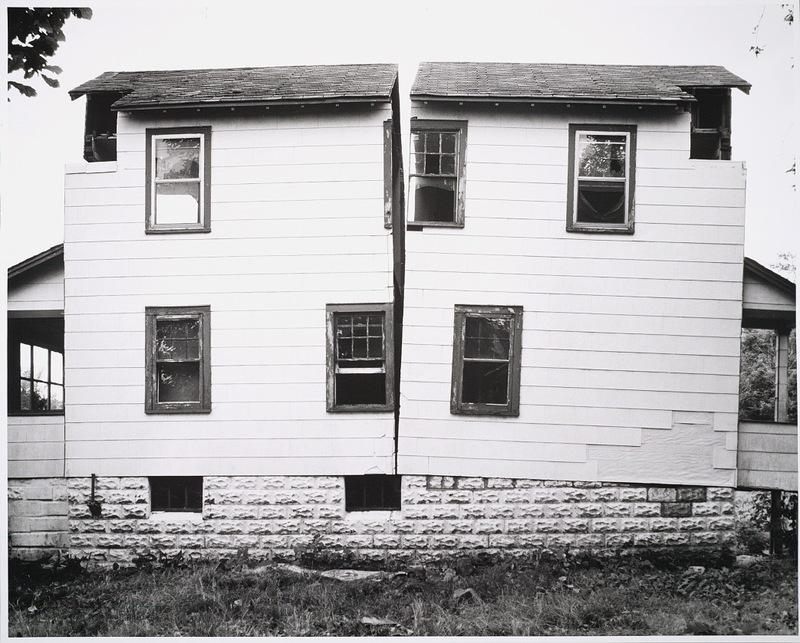
\includegraphics[width=85mm]{./imgs/cuts.jpg}
\caption{\tiny{\Formular{{\slsc{Building Cuts}}, de Gordon Matta Clark}}}
\end{figure}

\asterisc

O horror ao vazio e a política enquantro teatro"-peste são duas imagens em tensão, que atravessam este livro.

\chapter{A pedagogia do medo}

\section*{Proposta}

Este ensaio se divide em duas partes com diferentes pesos, que, a rigor, poderiam ser dois ensaios distintos. Decidi, porém,
articulá"-las em um mesmo texto na medida em que ambas abordam o
sentimento de medo no âmbito da arte de governo neoliberal. A proposta é
tentar examinar a questão de maneira mais livre, seguindo intuições e dando lugar
para que estas se desenvolvam.

Na primeira parte, tento elaborar o que poderia ser uma crítica
antropológica ao neoliberalismo, sob a perspectiva dos sentimentos de medo que
este engendra e a relação deste com formas de violência. Argumento que o medo emerge como operador da competição e
da concorrência, princípios basilares da visão de mundo neoliberal. O
medo é também o substrato por detrás da lógica de que o mercado tem uma
função pedagógica; sua capacidade não apenas de educar o ser humano,
como de desvendar a sua verdadeira humanidade --- esta imaginada como reflexo de
sua suposta natureza competitiva. Não é nada espantoso que sociedades
cujos valores mais elevados são a competição tenham também elevados
níveis de violência.

Esboço, na segunda parte, a eficácia que imagens violentas e corpos
mortos podem ter no interior dessa pedagogia do medo. Trata"-se de pensar
a ampla veiculação de imagens violentas, naquilo que elas buscam
produzir de sentimentos e modelos de ação no mundo.

De alguma forma, este ensaio não
passa de uma tentativa de refletir sobre a circulação de imagens na política
entendida como necropolítica --- na definição de Achille Mbembe --- a capacidade de subjugar a vida ao poder da morte, criando o
que o autor denomina ``mundos de mortes'', aos quais estão sujeitas partes
consideráveis do globo.

\pagebreak

\section*{Neoliberalismo e a educação~sentimental}
\addcontentsline{toc}{section}{\forceindent{}Neoliberalismo e a educação sentimental}

\epigraph{O sonho, que logo será interrompido brutalmente pelas trevas do
verdadeiro céu, desdobra a magia de um imenso espelho móvel e composto,
ele mesmo, de infinitas superfícies refletoras. Esses espelhos de pura
luz só podem brilhar no vazio, livres de opacidade. Os da vida presente
e terrena são diferentes: refletem lucidamente nossa sombra, quando em
nós cai a noite}{Jean Starobinski}

O que o medo pode nos revelar sobre a política? Um dos capítulos mais
recentes dessa relação histórica é o da governamentalidade neoliberal.
Proponho seguirmos a proposta de Isabelle Stengers e Philippe Pignarre em
\emph{A bruxaria capitalista} de definir as coisas não pelo o que elas
são, não uma definição pela sua essência, mas a partir de uma pragmática
cujo foco se desloca para o que criam, como agem. Assim, uma análise do
neoliberalismo sob o viés dos sentimentos que ele é capaz de engendrar ---
enfocando aqui o medo --- permite, acredito, compreendê"-lo em seu poder performativo de criar mundos, de inventar possíveis, e concretizá"-los ao dar"-lhes forma.

\asterisc

É na obra do Marquês de Sade que encontro um ângulo para me aproximar
do capitalismo como máquina cujo funcionamento depende intrinsecamente
da criação do medo. Para uns maldito, para outros delicioso (assim a ele
se referem os surrealistas franceses), o mundo que Sade cria a partir de
um olhar para o abjeto, para o violento escatológico, é o avesso do
mundo concebido pela boa política republicana. Na criação desse
mundo invertido, revelam"-se as violências não evidentes que estruturam o projeto
republicano francês.

A própria vida de Sade chama atenção: marquês decadente e imoral,
é condenado à prisão na Bastilha, símbolo do Antigo Regime, por crimes
violentos cometidos em meio a uma vida libertina. Parte de seus escritos
foram justamente produzidos nos períodos passados em prisões e
manicômios. \emph{120 dias de Sodoma}, obra em que trabalhara ao longo
de anos a fio, desapareceu, para o desespero do autor, durante a Queda
da Bastilha em 14 de julho de 1789, momento áureo da Revolução Francesa,
devendo Sade retomar a sua escrita internado em instituições
manicomiais.

\emph{A filosofia na alcova} é uma peça de teatro que leva a filosofia
iluminista e seus ideais de liberdade e igualdade para este
pequeno quarto adjacente à sala, também conhecido por ser utilizado como
refúgio para encontros sexuais. A própria alcova como um pequeno quarto
não oficial, ao lado da parte mais pública e visível de casas privadas,
concentra em si o movimento do livro de Sade: levar a filosofia de criação de
uma esfera pública que embasava a Revolução Francesa para esse lugar
recôndito, onde sua face não aparente possa ser explicitada.

A narrativa, então, se desenvolve a partir de um ritual de iniciação
sexual e erótica de Eugénie, uma jovem a quem a libertina Madame de
Saint"-Ange quer iniciar nos mistérios mais secretos de Vênus, junto a
alguns de seus amigos, entre eles Dolmancé, sodomita convicto, o mais
excessivo, abundante e profuso instrutor de orgias da França. Uma
verdadeira antipedagogia, avessa aos padrões de moralidade e
normalidade, tem lugar, implicando uma espécie de aprendizagem também aos
seus leitores, de ambos os gêneros, convidados a buscar na
história de Eugénie práticas libertinas como formas de libertação
de si.

Em meio a cenas de sexo desenfreadas e intermináveis, em que todas as
posições e formações possíveis são testadas, a narrativa se interrompe
para a leitura de um panfleto, trazido por Dolmancé. \emph{Franceses,
Mais um Esforço se Quiserdes Ser Republicanos}, propõe a
necessidade de uma refundação moral e uma sociedade sem Deus como passos
determinantes para a construção de uma sociedade igualitária. A ironia é
patente: Dolmancé o retira do bolso, em meio à orgia, após uma demanda
de Eugénie por instruções eróticas, trazendo"-o diretamente do Palácio da
Igualdade.

Onde a filosofia iluminista via os benefícios de uma vida comum baseada
em uma legislação que a todos garantisse igualdade, Dolmancé denuncia a
violência inerente a tais proposições. De modo absurdo, com traços que
serão posteriormente retomados pelos surrealistas, a voz de Sade se confunde
com a de Dolmancé, criticando um por um os
pontos do panfleto republicano. Em tom anticlerical, Dolmancé considera a
religião o maior inimigo da liberdade almejada, e critica sua transposição
para a educação cívica e à forma de culto laico ao Estado.

Nessa inversão, Dolmancé reivindica a prerrogativa de cometer atos
violentos como parte de sua liberdade, e acusa as violências arbitrárias
da imposição de modos de vida pela República. É toda a forma de
vida que a República Francesa deseja criar que, como em um jogo de
espelhos, emerge como violenta e desumana, pela denúncia feita
por um grupo de libertinos em meio a orgias.

A articulação entre
discurso da liberdade e práticas violentas e corporais cria em Sade uma
defesa radical da libertinagem como forma de vida ao questionar o
próprio programa de gestão da vida, da arte de governar esboçada pela
República em plena instauração. Trata"-se de um olhar sobre tudo que
excede os discursos políticos de sua época.

\asterisc

Inspirado menos pela temática orgiástica e mais por esse movimento de
Sade em \emph{A filosofia na alcova} de buscar as formas de violência
presentes nas propostas da arte de governar republicana, apresento
abaixo alguns aspectos do neoliberalismo enquanto máquina de criação de
formas de vida, nas quais medo e violência são constantes. Se a
concorrência é a base da governamentalidade neoliberal, ela só funciona
ao estimular o cultivo de sentimentos de medo frente ao outro.

Dito de outro modo, parto da ideia de
que o enfoque na própria estrutura do mercado como mediador de problemas
sociais, políticos e pessoais, amplamente embasado na concorrência e na
competição, não pode existir senão dependente do cultivo do medo como
produtor de subjetividades. A questão não é exatamente a existência do
medo ou não, mas o seu uso político em processos de assujeitamento no
interior da arte neoliberal de governar corpos. Mas antes, vale fazer um
breve contorno para explicitar, ainda que em sobrevoo, aquilo que certos autores críticos entendem como características políticas inerentes ao neoliberalismo --- dos quais trago inspirações para esta reflexão.

\asterisc

O desafio colocado por autores como Michel Foucault, Giorgio Agamben,
Sayak Valencia, Achille Mbembe, entre outros, consiste em pensar o
neoliberalismo para além das práticas pelas quais a agenda neoliberal se
traduz nos debates políticos ordinários --- usualmente marcada pela
dobradinha privatizações e redução do Estado como
forma de manutenção do mercado livre. O neoliberalismo, de acordo com o pensamento de Friedrich von
Hayek, vai muito além disso: almeja tornar"-se uma nova forma de entender
a maneira pela qual podemos conhecer o mundo.

Hayek acredita ter encontrado no Mercado uma maneira objetiva de observar, conceber e planejar o mundo. E a competição como a única forma legítima de organizar a sociedade. A fundamentação e
legitimação do Estado, para muitos neoliberais, não estaria nem na
classe (como desejavam os marxistas), nem na cultura ou raça (como
pretendiam os nazifascistas), mas na econômia ordenada pela livre
concorrência.

Segundo o escritor britânico Stephen Metcalf, trata"-se, para Hayek, da possibilidade de ``estruturar toda a realidade pelo modelo da competição
econômica''.\footnote{Disponível em: \textless{}{\slsc{https://bit.ly/2wg1bnN}}\textgreater{}.}
Como quase todas, senão todas, as atividades humanas tomam a forma do
cálculo econômico, então podem ser compreendidas com maior precisão a
partir de conceitos como riqueza, valor, troca, custo e, especialmente,
preço. Para que este sistema funcione, basta que as pessoas busquem os
seus interesses próprios, que são equacionados pelo mercado, gerando um
bem comum. Diferente do liberalismo clássico, regido pelo \emph{laissez"-faire},
o neoliberalismo demanda ativamente que o Estado crie as condições que
garantam a competição e o funcionamento dos mecanismos de precificação.

Michel Foucault, quando começa a se debruçar sobre a forma de governo
neoliberal, elabora o conceito de governamentalidade:

\begin{quote}
Por ``governamentalidade'' entendo o conjunto constituído pelas
instituições, procedimentos, análises e reflexões, os cálculos e as
táticas que permitem exercer essa forma bem específica, ainda que
complexa, de poder que tem por alvo principal a população, por forma
maior de saber a economia política, por instrumento técnico essencial os
dispositivos de segurança. Segundo, por ``governamentalidade'' entendo a
tendência, a linha de força que, em todo o Ocidente, não cessou de
conduzir, e desde muito tempo, à preeminência deste tipo de poder que
podemos chamar de ``governo'' sobre todos os outros: soberania,
disciplina, e que, por uma parte, levou ao desenvolvimento de toda uma
série de aparelhos específicos de governo {[}e, de outra parte{]}, ao
desenvolvimento de toda uma série de saberes.\footnote{\scalebox{.8}{FOUCAULT},
  Michel. {\slsc{Sécurité, territoire, population: cours au Collège de France,
      1977-1978}}. Paris: Gallimard/Seuil, 2004, p.~111-112 (trad.~minha).}
\end{quote}

O desafio para se compreender o neoliberalismo como uma arte de governo
específica, pela ótica da governamentalidade, diz respeito à forma de
gestão da vida, através da qual as pessoas passam a ser compreendidas como empresas em
incessante competição. Nesse âmbito, e em outro momento de sua
obra,\footnote{\scalebox{.8}{FOUCAULT}, Michel. {\slsc{O nascimento da biopolítica}}. São Paulo: Martins Editora, 2008.}
Foucault explora de que maneira o mecanismo disciplinar da loucura é
ampliado para formas de gestão da vida como um todo, para além dos manicômios. De certa forma, a gestão da
loucura é um laboratório para a gestão da vida. De maneira análoga, a gestão econômica e empresarial projetada pela
arte de governo neoliberal é ela mesma um exercício de formulação
para a gestão da vida.

Sayak Valencia, em \emph{Capitalismo gore}, e Achille Mbembe, em
\emph{Necropolítica}, promoveram um deslocamento analítico na forma como
o neoliberalismo vinha sendo criticamente analisado. Deixando de lado o
modelo biopolítico proposto por filósofos europeus como Michel Foucault
e Giorgio Agamben, Valencia e Mbembe ressaltam que as formas
de gestão da vida no neoliberalismo são indissociáveis das formas de
gestão da morte, da decisão entre quem vive e quem morre.

Existe uma realidade violenta que o neoliberalismo cria em suas margens,
ou em zonas específicas do globo, verdadeiras zonas extrativas de
recursos naturais, mão de obra barata, tempo e vida. Regiões que são
alheias à imagem que o neoliberalismo cria de e para si mesmo. Ou que não
parecem ter lugar nos discursos neoliberais sobre a forma de governo
proposta.

\asterisc

No mercado livre, em sua concepção neoliberal, a concorrência opera de
forma plena e possui potencial explicativo absoluto, tido como o
mecanismo mais eficiente para ordenação social e política. Por ele tudo
pode ser explicado, e funcionar perfeitamente, desde que as garantias da
livre concorrência estejam asseguradas. Ao Estado cabe, justamente,
assegurar que a livre concorrência entre partes tenha lugar, ainda que
para isso reelabore o seu aparato legal, com uma nova
correlação entre moral, ``normalidade'' e punição, para garantir que
partes não atrapalhem umas às outras na livre concorrência. É a própria
definição da economia como ``melhor forma de gestão de bens limitados''
que possibilita a lógica concorrencial.

O mercado ideal, e a economia política neoliberal, funcionam embasados
nesse idealismo; são forjados à imagem do conceito de guerra de todos
contra todos de Thomas Hobbes. Não se trata de uma guerra efetiva, mas
do cálculo diante da ameaça, da possibilidade do outro empreender uma
ação violenta contra mim. Na lógica dessa guerra, devo me armar e me
assegurar para, no caso dessa ameaça se tornar crível, poder dela me
defender. Essa imagem do Mercado como um estado de guerra que lhe
constitui à sua semelhança é naturalizada. Não se trata de uma opinião
política, nem de ideologia. Para os seus defensores, é um argumento
totalizante: essa é a realidade. O mundo simplesmente é assim, a
natureza é assim, e qualquer opinião divergente é uma visão política
ideológica, não natural, distorcida.

Os efeitos desse mecanismo competitivo à moda da guerra, sejam eles
sociais (como o aumento da desigualdade e da violência), sejam eles
subjetivos (como os altos índices de depressão, ansiedade e suicídios),
sejam eles ambientais, estão, a rigor, aquém da lógica do Mercado. São
presenças incômodas, pois ameaçam a coerência absoluta de seus axiomas.
E quando se inserem na lógica do Mercado, é para que partes possam obter
lucros, e criar novos nichos de competição: o mercado da segurança e dos
condomínios murados para lidar com a violência e a desigualdade, a
indústria dos antidepressivos para lidar com as subjetividades
destroçadas pela competição, os mercados de precificação de carbono para
lucrar com a crise ambiental.

Diante de um princípio lógico e coerente, sem nenhum tipo de
contradições ou ambivalências, como se apresenta o Mercado na visão de
Hayek, capaz de entender o mundo como se deve a partir do mecanismo de
precificação, o mundo palpável, sensível, vivível, é relegado a um
segundo plano; desmerecido, pois incoerente, contraditório e, de certo
modo, rebelde a leituras demasiado estáticas. Aos olhos do Mercado, a
busca por compreensão das volatilidades e contradições que marcam a
experiência de vida, do sensível, já não mais podem inspirar a
construção de uma política da vida comum.

O mercado, como uma utopia coerente, em que tudo faz sentido, converte o
mundo palpável, sensível, em uma verdadeira distopia.

\asterisc

Sentir medo é um estado afetivo corriqueiro, cotidiano, em nada
excepcional. Positivo, na medida em que associado a um estado de
autopreservação e cuidado de si. Entretanto, explorar o uso político do
medo como forma de subjugo e dominação abre perspectivas para o
entendimento do exercício do poder de mando e da arte de governo --- como o
fazem diversos filósofos políticos, como Hannah Arendt, em
\emph{Origens do totalitarismo}, acerca do nazifascismo europeu.

Enquanto sentimento, o medo é marcado por uma ambivalência,
definindo"-se como um ``estado afetivo suscitado pela consciência do
perigo ou que, ao contrário, suscita essa consciência'', segundo
o dicionário Houaiss. Ou seja, o medo é tanto fruto da
consciência do perigo como motivador dela. Tal definição aponta para
algo de forjado na sensação do medo, mas não por isso
menos real, já que concreto.

Proponho pensar o medo em contraste
com o estado melancólico, definido por uma
assincronia entre o tempo interior e o movimento das coisas exteriores.
A oscilação entre exaltação e abatimento produz a dinâmica melancólica.
O melancólico é aquele que ora aparece frenético, acelerado diante de um
tempo lento, pesado, imutável, por vezes sufocante, ora destruído por
sua incapacidade de interagir junto ao ``espetáculo exterior que se
acelera vertiginosamente''.\footnote{\scalebox{.8}{STAROBINSKI}, Jean. {\slsc{A melancolia
  diante do espelho}}. São Paulo: Editora 34, 2014, p.~59.}

Vale uma breve incursão em como a sensação de medo foi explorada pelo nazifascismo no século \versal{XX}, e em sua própria forma de produção. Não para traçar semelhanças ou afirmar que seja a mesma coisa, e sim para melhor apontar diferenças e particularidades em como o neoliberalismo reorganiza a sociedade a partir da ideia de competição e do uso político que faz do medo.

Esse estado de descompasso temporal entre o eu e o mundo, na oscilação
entre exaltação e paralisia, é um estado moderno por excelência,
reflexo da aceleração das
mudanças ocorridas entre o final do século \versal{XIX} e início do século \versal{XX}.
Essa oscilação sentimental própria da melancolia torna"-se um sentimento
básico a ser explorado pela política no século \versal{XX}, principalmente pelo
nazifascismo europeu, que depende da exploração dos sentimentos de ação
gloriosa, exaltação patriótica, transformação ativa de um mundo em
oposição à sua degeneração moderna, por um lado; e o estado estático,
imobilizado, subserviente, inerte, de cabeça baixa, consentindo a todo
tipo de violência, por outro.

Como forma de governo, o nazifascismo depende de uma verdadeira máquina
de produção de sentimentos.

\asterisc

Em \emph{O fim do homem soviético}, a jornalista e escritora Svetlana
Aleksiévitch reconta a história do stalinismo e seus efeitos na sociedade
soviética a partir das memórias de medo e violência sofridas pela
população. A autora relata, surpreendentemente com um tom nostálgico, as
conversas em tom de fofocas políticas na União Soviética, em que
famílias inteiras, compartilhando apartamentos abarrotados e com medo de
telefones grampeados, ligavam a televisão bem alta, e iam à cozinha
falar mal do Estado e seus governantes. Soube"-se depois que o próprio Stalin se valia dessa
técnica, com receio de ser traído pelas escutas em seu telefone. De
acordo com diversos historiadores, os expurgos políticos realizados por
Stalin, com assessoria de seu temerário aliado Lavrenti Beria, teriam
sido catalisados tanto pelo medo que tinha Stalin de Beria, como pelo
medo de Beria por Stalin.

No totalitarismo nazisfacista, o medo é reificado, ganha uma realidade
para além das pessoas e dos lugares por elas ocupados. Os homens eram,
em suma, tornados supérfluos, como bem argumenta Hannah Arendt em
\emph{Origens do totalitarismo}:

\begin{quote}
A diferença fundamental entre as ditaduras modernas e as tiranias do
passado está no uso do terror não como meio de extermínio e
amedrontamento dos oponentes, mas como instrumento corriqueiro para
governar as massas perfeitamente obedientes. O terror, como o conhecemos
hoje, ataca sem provocação preliminar, e suas vítimas são inocentes até
mesmo do ponto de vista do perseguidor (\ldots{}) leva à situação na qual
jamais ninguém, nem mesmo o executor, está livre do medo.\footnote{\scalebox{.8}{ARENDT},
  Hannah. {\slsc{Origens do totalitarismo}}. São Paulo: Companhia das Letras, 2012, p.~29-30.}
\end{quote}

\asterisc

``Mesmo uma paisagem tranquila\ldots{} mesmo uma pradaria com voo de corvos,
com montes de ervas\ldots{} mesmo uma estrada onde passam carros, camponeses,
casais\ldots{} mesmo um vilarejo de férias com um campanário, podem
simplesmente conduzir a um campo de concentração''. Essa frase é
narrada no filme \emph{Noite e neblina} (1955), de Alain Resnais, em voz over,
enquanto a imagem de uma pradaria aparentemente pacata e vazia revela
aos poucos, acompanhando a fala, a existência dos resquícios de um campo
de concentração. O filme concentra em 32 minutos um dos momentos mais
perturbadores da história do cinema: uma imagem que se constrói entre a
necessidade ética e política de dar forma e tornar visível o horror do
genocídio judaico do século \versal{XX}, por um lado, e a sensação de
insuficiência, de que seria impossível imagens apresentarem o que foram as máquinas da morte.

O filme foi lançado cerca de dez anos depois da queda do nazismo, a dificuldade de
se acreditar que existiu nesses amplos descampados um campo de
concentração é similar à dificuldade de entendê"-los como produto de uma
sociedade determinada, de pessoas de carne e osso, que saíam da
administração de Auschwitz e iam jantar com suas famílias e cuidar dos
seus filhos. \emph{Noite e neblina} não exibe nem recria cenas de
assassinato coletivo. O que é mostrado são as reminiscências do
extermínio: as imagens impactantes feitas pelos aliados sobre os montes
de corpos, as estruturas do campo de concentração vazias, sem
prisioneiros, delineando a difícil barreira a ser transposta, a
dificuldade de se ter uma imagem da rotina, da vida nos campos da morte.

O filme tenta tornar público, tornar visível para o espectador, aquelas
estruturas que haviam sido planejadas, através de todos os dispositivos
políticos, arquitetônicos e engenheirísticos então disponíveis, para
tornarem invisível o que acontecia nos campos de concentração. Toda a
tecnologia da época estava disponível para auxiliar que o inimaginável,
o extermínio industrial de toda uma população, tivesse lugar.

A contrapelo, Resnais evidencia aquilo que o nazismo tem
em comum com os modos de produção de mercadorias pelo capitalismo na
primeira metade do século \versal{XX}. A organização industrial da morte em
campos de concentração obedece ao mesmo princípio de racionalidade e
maximização do lucro que qualquer outra atividade comercial ou
industrial. Havia concorrência entre as empresas dispostas a prestar
seus serviços, e cálculos racionais objetivando maximizar a produção da
morte e reduzir custos: matar mais, gastando menos, diminuindo o
sentimento de culpa do assassino através de uma tecnologia que
despersonificava o ato de matar e, por fim, utilizando os resquícios dos
corpos como matérias"-primas para objetos industriais.

Os corpos dos
mortos, nos campos de concentração, têm uma função produtiva, mostram as
imagens do filme, sempre em número industrial, sem personificar nem
individualizar, ao focalizar as pilhas descomunais de cabelos e
vestimentas. O cabelo dos exterminados converte"-se em cobertores e
agasalhos; a pele em papel; a gordura em sabão; os ossos em adubo para a
terra. Essa terra adubada com os corpos esfacelados que, justamente,
fertilizada, permitiu o crescimento da relva que esconde os campos de
concentração que ali existiam. \emph{Business as usual} é uma das
facetas mais perversas da máquina de morte nazista.

Para Hannah Arendt, uma das dimensões para compreensão do genocídio
judaico no século \versal{XX} é o fato de que, pela primeira vez, aquilo que era
feito pelos europeus nas colônias se realizava em tamanha escala no
Velho Continente. Como coloca Mbembe, a partir da reflexão de Enzo
Traverso:

\begin{quote}
Segundo Enzo Traverso, as câmaras de gás e os fornos foram o ponto
culminante de um longo processo de desumanização e de industrialização
da morte, entre cujas características originais estava integrar a
racionalidade instrumental com a racionalidade produtiva e
administrativa do mundo ocidental moderno (a fábrica, a burocracia, a
prisão, o exército). Mecanizada, a execução em série transformou"-se em
um procedimento puramente técnico, impessoal, silencioso e rápido. Esse
processo foi, em parte, facilitado pelos estereótipos racistas e pelo
florescimento de um racismo baseado em classe que, ao traduzir os
conflitos sociais do mundo industrial em termos raciais, acabou
comparando as classes trabalhadoras e os ``desamparados pelo Estado'' do
mundo industrial com os ``selvagens'' do mundo colonial.\footnote{\scalebox{.8}{TRAVERSO}, Enzon. In: \scalebox{.8}{MBEMBE},
  Achille. ``Necropolítica''. Revista {\slsc{arte e ensaio}}. Rio de Janeiro:
  \scalebox{.8}{UFRJ}, número 32, 2016.}
\end{quote}

O capitalismo encontra no nazismo não a sua exceção, mas o ponto de
indistinção entre a normalidade da produção e a mercantilização
coisificada da vida. A necropolítica como base do capitalismo. A
soberania compreendida como capacidade de permitir viver e decidir
matar. O pensamento nazista, fazendo coincidir a figura do ``outro''
judeu com a do comunista, não via outra saída senão eliminá"-lo, para
impedir que um outro futuro possível pudesse ter lugar. A violência e o
genocídio, aos olhos nazistas, assumia uma função criadora, capaz de dar
luz a um novo mundo.

\asterisc

O neoliberalismo, como arte de governo, cria uma narrativa totalmente
distinta do nazifascismo europeu, no que diz respeito à produção de
subjetividades. No lugar da subsunção às massas sem sujeitos, o neoliberalismo
segue o caminho oposto, o da exacerbação de individualidades, desejos,
gostos, sonhos\ldots{} medos. Afetividades padronizadas, mas de maneira
distinta àquela da indefinição das massas, do controle totalizante de
sentimentos pelo terror. Uma mudança concreta no peso atribuído aos
sentimentos em expansão. Uma nova educação sentimental, em que o cultivo
do medo muda de aspecto. Emerge uma lógica da individualização da culpa
e do fracasso, segundo os ditames da concorrência do sistema econômico,
para o qual o sucesso na vida depende exclusivamente de cada pessoa.
Estar sempre em competição, em concorrência, em dívida sobre quem cada
um ``deve ser''.

A própria noção de pessoa muda. Da pessoa alienada de seu trabalho pelos
resultados e alienada de si mesma, para a não menos perversa noção de
pessoa como empresa de si. A estrutura de mercado assegura às pessoas
um lugar específico, uma possibilidade de ação delimitada, na qual
exaltação e excitação, que marcam um dos polos da melancolia, devem ser
contidas, domesticadas, e se exacerba a possibilidade de inação, fixidez
e autocontrole.

Ainda no campo da melancolia, vale lembrar a lição de Starobinski sobre
Baudelaire no final do século \versal{XIX}, que parece nos dizer algo sobre a
lógica de autopunição de uma vida baseada na competição:

\begin{quote}
a relação
consigo mesmo suplantou a relação com outrem: para tanto, terá ocorrido
o desdobramento graças ao qual \emph{castigar a si mesmo} torna"-se um
gesto representável, homólogo e inverso ao gesto de castigar a
outrem.\footnote{\scalebox{.8}{STAROBINSKI}, op.~cit., p.~33.}
\end{quote}

\asterisc

Voltemos, agora, às relações entre mercado, competição e proliferação da violência.
A absolutização do mercado como princípio operador, gerenciador e
gerador da realidade, implica também uma pedagogia, ao ensinar
possibilidades e modos de agir no mundo. É a predação e o medo das
possibilidades de agressão do outro que demandam o estudo das
possibilidades de ação; o cálculo entre precaução e agressão como
princípio da racionalidade de ação. O medo, em suma, é o sentimento que
permite à competição funcionar, estrutura o mercado e, por isso, mostra ao humano
sua verdadeira essência natural e competitiva.

Na perspectiva do mercado, é a imagem de uma natureza
predatória que serve de inspiração para essa antropologia essencialista
do humano; que mais parece ser a projeção, o reflexo de como esse
sistema sociopolítico produtivo imagina a si próprio.

A antropóloga sino"-estadunidense Anna Tsing estabelece uma correlação entre
concentração de poder estatal, ascensão do patriarcado e o
desenvolvimento de monoculturas a partir da perspectiva dos fungos. As
monoculturas se tornam mais suscetíveis ao poder destrutivo dos fungos,
o que despotencializa a capacidade de interação dos fungos com outras
espécies que gera uma profusão de formas de vida. Segundo Tsing, isso
implica uma maior demanda de trabalho dos humanos, que passa a ser
controlado por homens fortes, resguardando às mulheres funções
domésticas.

\begin{quote}
A interdependência entre as espécies é um fato bem conhecido --- exceto
quando diz respeito aos humanos. \emph{O excepcionalismo humano nos
cega}. A ciência herdou das grandes religiões monoteístas narrativas
sobre a superioridade humana. Essas histórias alimentam pressupostos
sobre a autonomia humana e levantam questões relacionadas ao
\emph{controle}, ao \emph{impacto} humano e à natureza, ao invés de
instigar questões sobre a interdependência das espécies. A ideia de
natureza humana foi apropriada por ideólogos conservadores e por
sociobiólogos que se utilizam de pressupostos da constância e autonomia
humanas para endossar as ideologias mais autocráticas e militaristas. E
se imaginássemos uma natureza humana que se transformou historicamente
com variadas teias de dependência entre espécies?\footnote{\scalebox{.8}{TSING},
  Anna. ``Margens indomáveis: cogumelos como espécies companheiras''. {\slsc{\scalebox{.8}{ILHA}}}, v.~17, n.~1, p.~177-201, jan./jul. 2015, p.~184.}
\end{quote}

\asterisc

Em um texto opinativo publicado por Malcolm Harris na \emph{Al Jazeera},\footnote{\scalebox{.8}{HARRIS}, Malcolm. \mbox{Disponível em: \textless{}{\slsc{https://bit.ly/2V9yULe}}\textgreater{}.}}
em dezembro de 2015, o autor busca uma explicação cultural para as
massivas matanças com armas nos Estados Unidos. Harris cita jovens norte"-americanos entre 21 e 26 anos que presenciaram tiroteios, e cujas
falas foram compiladas para o livro de outros dois jornalistas. Harris
enfoca na diferença de perspectiva entre a geração dos jornalistas e a
dos jovens que vivenciaram situações de massacre, muito mais aptos à
compreensão do fenômeno do que os jornalistas.

Uma dessas pessoas, de 26 anos, afirma: ``é a sociedade como um
todo que está em conflito consigo mesma''. Outro jovem, também de 26
anos, faz uma reflexão sobre a pressão que existe na promoção da
competição desde pequenos: ``siga esse caminho até o fim e você ganha.
Siga aquele outro caminho, e você não é ninguém. A pressão para vencer
está em todos os lugares. Paira sobre nós, empurrando para baixo, desde
a escola. A sensação é que você está em uma batalha pela sua
sobrevivência, mesmo que você tenha recursos
financeiros''.

O autor do artigo conclui, evidenciando a relação entre
competição, medo e violência: ``em uma sociedade que opõe cada criança
com o mundo todo por espaços de sucesso em diminuição, fuzilar a sua
escola parece quase um mal entendido. Supõe"-se que você irá matar os
seus colegas de classe apenas de maneira figurativa'', afirma
Harris.

\asterisc

Em junho de 2016, o Fundo Monetário Internacional publicou um artigo
intitulado \emph{Neoliberalism: Oversold?} (\emph{Neoliberalismo:
superestimado?}, em tradução livre), assinado por economistas
experientes do órgão.\footnote{Disponível em: \textless{}{\slsc{https://bit.ly/2PASiOL}}\textgreater{}.}
O artigo tem como pano de fundo a discussão sobre o sucesso das medidas
neoliberais adotadas pelo governo chileno. Em 1982, Milton Friedman
teria declarado o caso chileno como um ``milagre econômico'', a ser
exportado mundo afora. Segundo Friedman, a dobradinha aumento da
competitividade com diminuição do Estado estaria na origem desse
sucesso, e se transformaria em uma fórmula a ser vendida mundo afora.
Os autores questionam, sempre tendo o caso do Chile em mente, o real
sucesso da implementação da agenda neoliberal, a partir de três pontos:

\begin{enumerate}[label=\roman*.]
%\def\labelenumi{\alph{enumi})}
\item 
  a dificuldade de estabelecer uma correlação entre aumento do
  crescimento e medidas neoliberais quando se olha para um grande grupo
  de países;
\item 
  o elevado custo decorrente do aumento da desigualdade;
\item 
  o próprio aumento da desigualdade originado nas medidas da agenda
  neoliberal coloca em xeque a manutenção do suposto crescimento
  neoliberal.
\end{enumerate}

O artigo foi publicado pelo \versal{FMI}, o maior promotor de medidas
desregulatórias e incentivador da competição. Entre os questionamentos
levantados pelo experiente time de economistas, que mostram a
fragilidade da agenda neoliberal, não se leva em consideração, em nenhum
momento, questões como violência, ditadura ou direitos humanos.
Esquecem de um aparente mero detalhe para eles: o ``milagre econômico''
chileno aconteceu em meio a uma das maiores atrocidades do século \versal{XX}. A
invisibilidade, a ausência de um processo político como a ditadura
chilena no debate econômico, evidencia o desmerecimento da realidade
experienciada que marca o pensamento neoliberal.

\asterisc

No filme \emph{O ato de matar} (2012), de Joshua Oppenheimer, Christine
Cynn e um diretor indonésio que preferiu manter o anonimato, os
diretores tratam do genocídio perpetrado pelos militares indonésios
contra a população chinesa de seu país. Contando com a aprovação de grande parte
da população indonésia, estima"-se que em um ano foram mortos mais de um milhão de
indonésios de origem chinesa que, por sua origem étnica, eram identificados como comunistas.

\begin{figure}[!ht]
\centering
 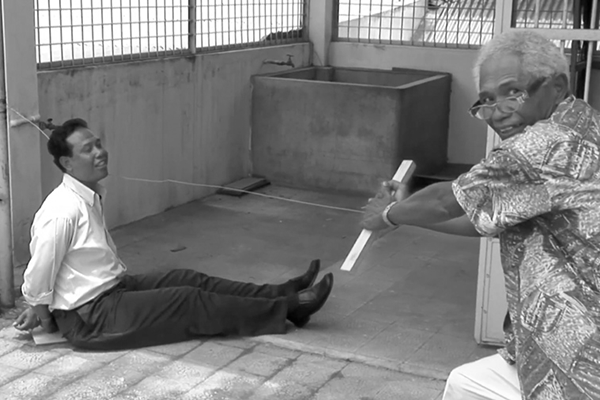
\includegraphics[width=85mm]{./imgs/frame1.png}
\caption{\tiny{\Formular{Anwar Congo encena como realizava o assassinato de indonésios de origem chinesa. {\slsc{Frame}} do filme o {\slsc{Ato de matar}} (2012)}}}
\end{figure}


A personagem central do documentário é Anwar Congo, um ex"-vendedor de ingressos de
cinema no mercado ilegal que, durante os eventos que se seguiram à
tentativa de golpe militar em 1965, passa a trabalhar como gangster
junto a seus comparsas, no extermínio da população chinesa. Congo e seus
companheiros são celebrados como grandes heróis da nação indonésia por
tê"-la salvado do comunismo, e são reverenciados como os pais fundadores
dos paramilitares, que até hoje detêm grande poder no país, possuindo vínculos
estreitos com o governo institucional.

Congo toma parte em um filme rodado dentro do documentário, no qual se
vangloria dos seus feitos: dança e sorri enquanto recria o modo como
matava e torturava; disfarça"-se de cowboy americano ou de gangster para
parecer um herói de filmes hollywoodianos. O espectador é
colocado em uma situação incômoda, de incompreensão frente a um grande
genocida sendo celebrado como símbolo de uma nação, que o vê como um
exemplo de homem livre.

\emph{O ato de matar} possui múltiplas camadas que tornam difícil de
entender as fronteiras entre o documental e a encenação do filme criado
por Anwar Congo e seus aliados --- como se fosse impossível aludir a
esse genocídio sem trazer para a própria forma do filme essa confusão
entre ficção e realidade. Anwar e sua gangue passam boa parte do tempo
discutindo as melhores maneiras de expor nas telas as mortes que
realizaram: como fazer durar, do modo mais realista possível, as imagens
daqueles que salvaram o país? Parece ser essa a questão que lhes move.

Depois de certo ponto, começam também a refletir sobre os fantasmas
daqueles que assassinaram, e que seguem perturbando"-lhes. Ao espectador
é impossível saber se estão atuando ou se existe uma experiência
traumática que compartilham em momentos de reflexão, uns com os outros.
Os genocidas aqui são apresentados em sua intimidade mais humana,
naquilo que existe de mais desconfortável em reconhecer um ser humano no
genocida. Seu passado, seus pesadelos, seus medos.

\asterisc

Em conversa junto à revista \emph{Vice}, o entrevistador pergunta a Joshua
Oppenheimer como teria conseguido a cumplicidade de Congo e seus
comparsas para se exporem de tal modo na realização de um filme em que
eles reivindicam serem perpetradores de um genocídio. A resposta de
Oppenheimer choca pela sua singeleza, e nos diz algo para além do
contexto indonésio: os assassinos se vangloriam na frente da câmera
pois não acreditam que tenham feito nada de errado. Esse talvez seja o
limite último da relação entre visibilidade e invisibilidade da
violência, alheia a qualquer lógica ética.

\asterisc

O desafio que me coloquei aqui foi o de olhar para a violência do século \versal{XX}, o século mais sangrento
da história, segundo Eric Hobsbawm, um de seus mais proeminentes
prosadores, não como algo superado, deixado para trás. Olhar para a
violência do século \versal{XX} pela perspectiva de uma arqueologia da violência
neoliberal. O modelo da arqueologia, da investigação por fragmentos
destroçados, permite compreender melhor a conversão da vida em ``mundos
de morte'', e os efeitos diretos de uma lógica da competição forjada às
sombras de uma potencial guerra de todos contra todos. Efeitos que o neoliberalismo
desejaria borrar da imagem que constrói de
si, mas que insistem em irromper.

\pagebreak
\thispagestyle{empty}

\begin{vplace}[.6]
\begin{figure}[!ht]
\centering
 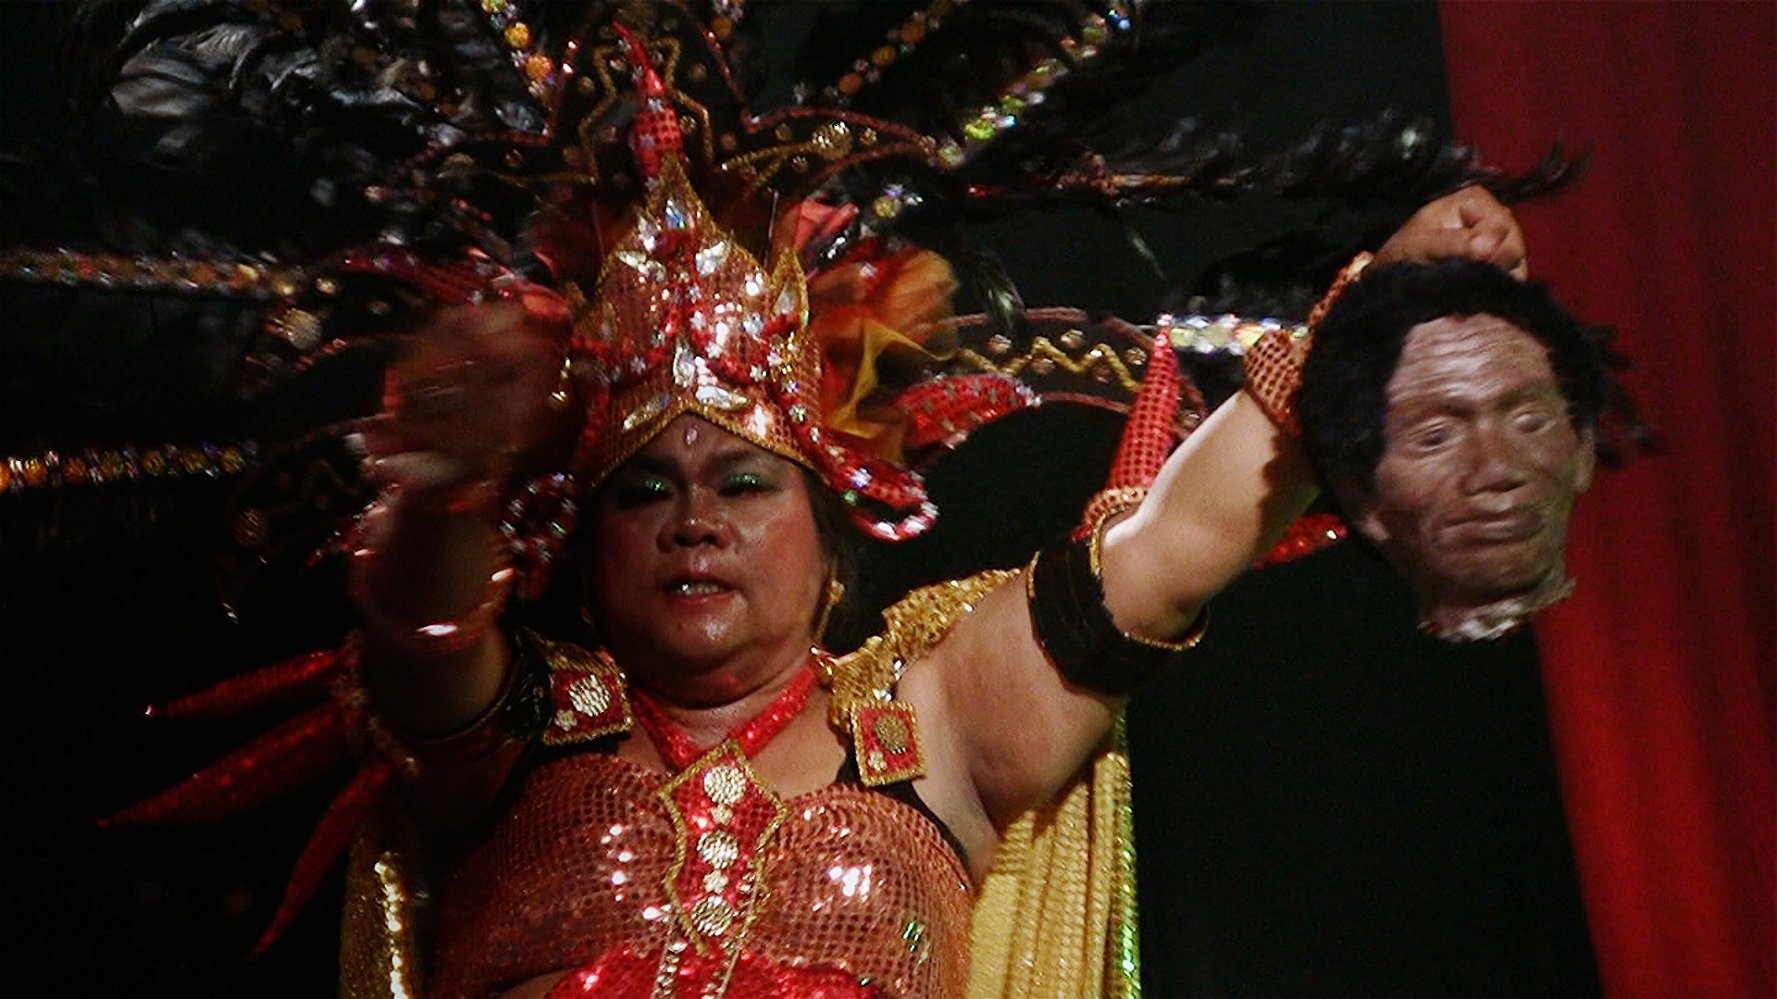
\includegraphics[width=85mm]{./imgs/frame2.jpg}
\caption{\tiny{\Formular{Frame de {\slsc{O ato de matar}} (2012)}}}
\end{figure}
\end{vplace}

\pagebreak

\section*{Pequena teoria visual do medo}
\addcontentsline{toc}{section}{\forceindent{}Pequena teoria visual do medo}

\epigraph{To display the dead, after all, is what the enemy does}{Susan Sontag}

A segunda parte deste ensaio começou a ser pensada em 2015, logo após a
abertura de uma exposição em que trabalhei como curador junto a duas
colegas e amigas --- Isabella Rjeille e Mariana Lorenzi. \emph{Frente à
euforia} reunia trabalhos de cerca de quinze artistas brasileiros/as e
colombianos/as, e investigava as diferentes maneiras pelas
quais o passado de violência extrema aparece em uma certa produção artística
recente destes dois países.

Longe de buscar um panorama representativo da produção artística local,
ou de defender a tese de que existiria uma ruptura inequívoca e radical
com relação ao passado, a proposta consistia em selecionar trabalhos de
algum modo reticentes ao discurso progressista e de otimismo muitas
vezes reivindicado pelos governos latino"-americanos no início do século
\versal{XXI}. A exposição explorava as contradições de tais processos, ao adentrar
o imaginário das transformações experimentadas com a diminuição da
pobreza e da desigualdade no Brasil e o ``pós"-conflito'' colombiano.
Euforia e fragilidade figuravam como sentimentos inerentes a essas
transformações, que pareciam prestes a se desfazer, a se estatelar no
chão. Evidentemente, não tínhamos dimensão, e nem sequer podíamos
conceber, até que ponto o fim desse período de otimismo traria à tona
fantasmas que queríamos há muito sepultados, pelo menos no caso
brasileiro.

Os comentários de Otávio Penteado, amigo antropólogo, encontram"-se na origem deste ensaio. Ele compartilhou comigo um desconforto quanto à nossa decisão
curatorial sobre o modo de exibir uma obra de Veronica Stigger, que denunciava a violência contra indígenas. Em sua instalação intitulada \emph{Menos um (Segunda
volta à cena do crime: Oswald de Andrade)}, montamos junto com Veronica,
em uma pequena sala do espaço expositivo, quatro enormes fotografias
impressas em alta resolução em que figuravam indígenas
violentamente assassinados, sendo um \emph{suicidado}, como bem coloca a
artista e escritora.

As imagens foram exibidas sem censura --- apenas com um pequeno aviso na
entrada, indicando que se tratavam de fotos violentas. Nelas estavam
dispostos corpos mutilados, empalados, com ossos quebrados, repletos de
sangue ou órgãos como o cérebro escorrendo pela cabeça rachada.
Concomitante e em \emph{looping}, ouvia"-se de um aparelho de som frases
de racismo e ódio compiladas por Veronica de comentários de leitores de
jornais de grande circulação que veiculavam notícias sobre assassinatos
de indígenas. Estes eram chamados de vagabundos, preguiçosos, e muitos
leitores pregavam a sua expulsão do país, assassinato e extermínio.

Provavelmente a peça de Veronica era não apenas a mais forte e
violenta da mostra, como também a que mais gerava horror. Aquilo que
havia perturbado Otávio era, precisamente, o modo como
aqueles corpos, vítimas de uma violência desmesurada, estavam dispostos
para tocar e sensibilizar a audiência da mostra.

Esse incômodo, de certa forma,
tornou"-se bom para pensar as tensões envolvidas nas diferentes
estratégias de empreender uma crítica visual e sensorial da violência.
Parte do texto está centrada em uma reflexão acerca das contradições do
tornar visível; mesmo quando se trata de uma exposição da violência que
visa denunciá"-la.

Esse ensaio se caracteriza principalmente por um vai e
vem histórico e geográfico, tendo como fio condutor questionamentos
sobre o medo, o terror e a visualidade da violência. No cruzamento entre
reflexões próprias aos campos da arte, da antropologia e do pensamento
político, esboça"-se uma teoria visual das sensações de terror.

Inicio pela forma como a arte renascentista se propunha
ser fonte de conhecimento, mnemônica e de geração de sentimentos de
piedade e comoção. Acredito que uma teoria visual dos sentimentos, tal
como esboçada no Renascimento, pode ser útil para investigar a
visualidade da violência hoje. Em seguida, passo pelo modo como certas
pesquisas antropológicas analisaram a relação entre a imagem do
\emph{outro} e a violência implicada na \emph{cultura do terror}, para
então me aproximar de uma reflexão acerca das distintas estratégias para
denunciar a violência.

\asterisc

No final do século \versal{XIII}, o teólogo e gramático Giovanni de Gênova
(também conhecido como Giovanni Balbi), escreve o \emph{Catholicon}, uma
gramática latina também identificada pelo nome de \emph{Summa
Grammaticalis}. Nela, preconiza uma tripla função das imagens
religiosas:

\begin{quote}
Sabeis que três razões têm presidido a instituição de imagens nas
igrejas. \emph{Em primeiro lugar}, para a instrução das pessoas simples,
pois são instruídas por elas como pelos livros. \emph{Em segundo lugar},
para que o mistério da encarnação e os exemplos dos santos pudessem
melhor agir em nossa memória, estando expostos diariamente aos nossos
olhos. \emph{Em terceiro lugar}, para suscitar sentimentos de devoção,
que são mais eficazmente despertados por meio de coisas vistas que de
coisas ouvidas.\footnote{\scalebox{.8}{GÊNOVA} apud \scalebox{.8}{BAXANDALL}, Michael. {\slsc{O olhar renascente: pintura e experiência social na Itália da Renascença}}. Rio de Janeiro: Editora Paz e Terra, 1991, p.~49.}
\end{quote}

\begin{figure}[!ht]
\centering
 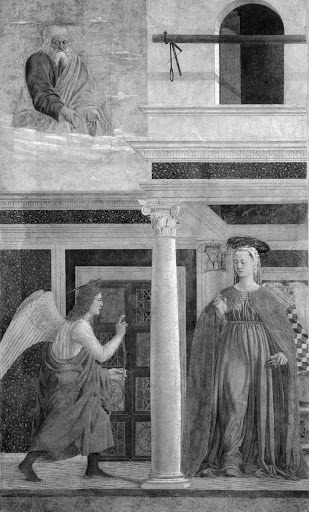
\includegraphics[width=85mm]{./imgs/francesca.jpg}
\caption{\tiny{\Formular{{\slsc{Anunciação}}, de Piero Della Francesca. Afresco na Basilica di San Francesco, Arezzo - Itália}}}
\end{figure}

A obediência das imagens religiosas produzidas na Igreja
a essas três funções disseminou"-se em parte das reflexões
sobre o fazer artístico no fim da Idade Média e durante o Renascimento,
e é presumível que os artistas tivessem"-nas em mente no momento de
elaboração de suas obras. Segundo o historiador da arte britânico
Michael Baxandall, seguir essas três regras significava produzir obras
cujo conteúdo fosse: em primeiro lugar, claro; em segundo, atraente e de
fácil memorização; e em terceiro, que se constituísse como representação
tocante de histórias sacras.

Meu objetivo não é realizar uma leitura precisa do modo como as pinturas
renascentistas partiam dessas três regras como princípios elementares de
sua composição pictórica --- para os leitores interessados remeto à
leitura de Baxandall acerca das pinturas sobre a \emph{Anunciação} e aos
estudos de Carlo Ginzburg sobre Piero della Francesca.\footnote{\scalebox{.8}{GINZBURG},
  Carlo. {\slsc{Investigando Piero: o Batismo, o ciclo de Arezzo,
    a Flagelação de Ulbino}}. São Paulo: Cosac \& Naify, 2010.}

Busco destrinchar o que poderia ser concebida como uma pedagogia dos
sentimentos que se dá por meio destas pinturas.


Nesse sentido, cabe atentar para mais uma reflexão teológica sobre a
imagem, desta vez trechos do sermão do dominicano Fra Michela Carcano,
proferido em 1492, que exploram a predominância do visual nos estímulos
à comoção:

\begin{quote}
As imagens eram introduzidas em virtude de nossa apatia
emocional; pois aqueles que não são levados pela devoção quando ouvissem
as histórias dos santos poderiam ao menos se comover quando as vissem
(\ldots{}) nossos sentimentos são estimulados por coisas vistas mais do que
por coisas ouvidas. \emph{Terceiro}, eram introduzidas porque muitas
pessoas não conseguem reter o que ouvem, mas se recordam quando as
veem.\footnote{\scalebox{.8}{CARCANO} apud \scalebox{.8}{BAXANDALL}, Michael, op.~cit.}
\end{quote}

Talvez seja possível estabelecer uma reflexão sobre a circulação de
imagens violentas hoje tomando como ponto de partida uma teoria visual
dos sentimentos esboçada por tais escritos teológicos. Os textos
teológicos que compreendiam a arte pictórica como detentora de elementos
para o exercício do poder eclesiástico e feudal através de
\emph{histórias bíblicas como modelos de ação no mundo} parecem ser
fontes incontornáveis para questões como: o que significam as imagens
religiosas no Renascimento? Como eram vistas? A que serviam? O que as
pessoas pensavam quando as viam?

Questões para uma reflexão política atual da relação entre imagens e
violência poderiam ser elaboradas de maneira análoga: o que significa a
proliferação de imagens violentas hoje? Como são vistas? Ou mesmo,
seguindo a formulação de Baxandall: que tipo de imagem violenta pode ser
considerada lúcida, de forte memorização e tocante? E principalmente, a
que servem? Em suma, se em sua função pedagógica a Igreja
buscava com a pintura estimular sentimentos de devoção e
piedade, ensinar e memorizar, quais sentimentos são hoje estimulados
pela proliferação de imagens violentas?


\begin{figure}[!ht]
\centering
 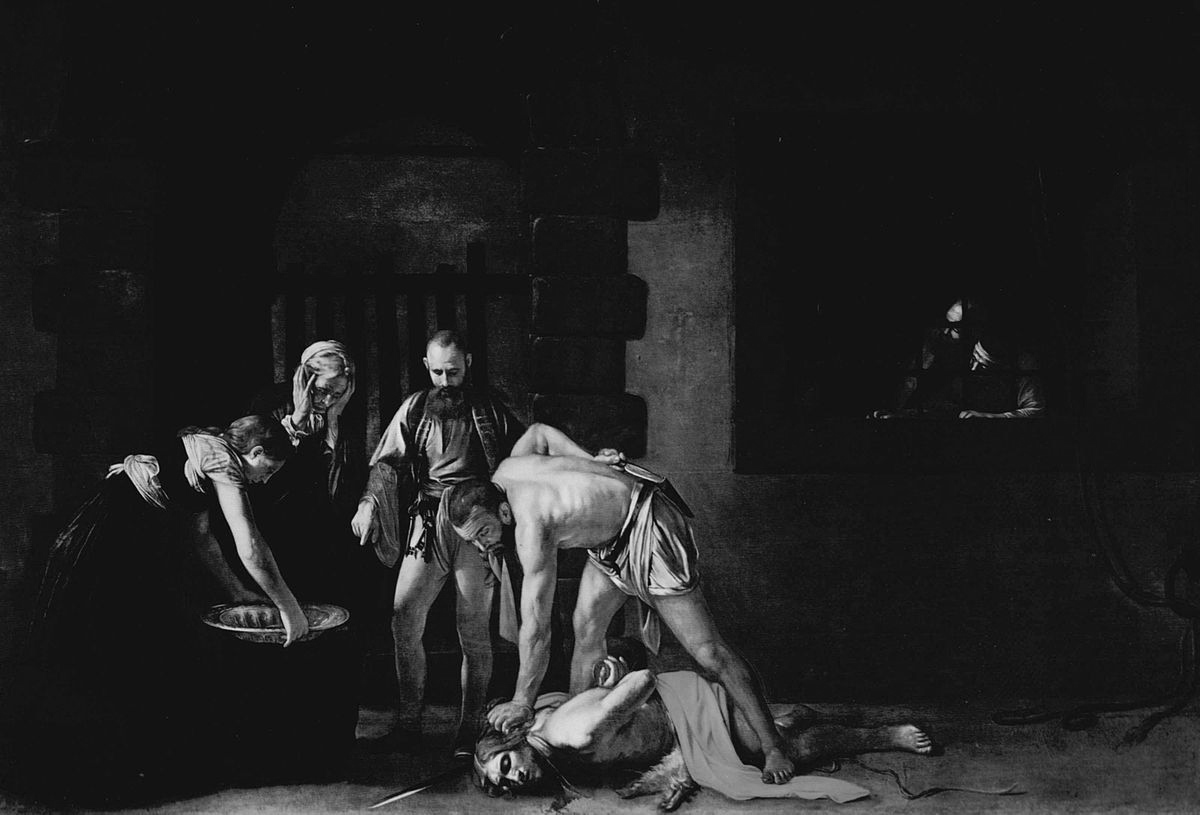
\includegraphics[width=85mm]{./imgs/decapitacao.png}
\caption{\tiny{\Formular{{\slsc{A decapitação de São João Batista}}, de Giovanni Caravaggio}}}
\end{figure}

\asterisc

Durante o \emph{Quattrocento}, a então nascente burguesia comerciante
florentina criou todo um novo imaginário para justificar a
posição singular que essa classe pleiteava criar, e que passa a ocupar.
Isso se dá por meio de uma leitura particular da Antiguidade, e toma a
forma de esculturas e pinturas --- uma leitura do passado antigo em
estreita relação com os valores então pregados por essa classe em
ascensão.

Como coloca Aby Warburg, o multifacetado historiador social da arte
renascentista, ``com Lourenço, o Magnífico {[}Lourenço de
Médici{]}, pela primeira vez o tipo do chefe político igual ao senhor
feudal e ao rei, se constrói a partir do comerciante urbano''.\footnote{\scalebox{.8}{WARBURG}, Aby. {\slsc{Essais florentins}}. Paris: Klincksieck, 2003, p.~117 (trad.~minha).}
Os retratos de Lourenço de Médici realizados por Ghirlandaio
apresentam"-no como um homem pleno e consciente, que começa a se
``destacar de seu plano de fundo religioso'',\footnote{Idem, p.~123.}
como quando o artista retrata a presença de seu mecenas na cerimônia de
aprovação que São Francisco recebe do Papa para conduzir a sua própria
ordem.

De acordo com Philippe"-Alain Michaud, em comentário à obra de Warburg,
para o autor alemão não se trata de encontrar semelhanças entre as obras
da Renascença e os seus ``modelos'' antigos. O que parece interessar a Warburg é o modo como a experiência moderna artística florentina se exprime a partir de uma identificação com o passado.\footnote{\scalebox{.8}{MICHAUD}, Philippe"-Alain. {\slsc{Aby
  Warburg et l'image en mouvement}}. Paris: Éditions Macula, 2012.}
Em um dos mais belos ensaios de Warburg, acerca da
\emph{Vênus} de Botticelli, o historiador busca entender os elementos da
Antiguidade que interessavam aos artistas do \emph{Quattrocento} --- no
caso desta obra"-prima renascentista, o autor alemão identifica"-os no
movimento de detalhes inanimados, como cabelos e vestimentas.

A leitura de Warburg acerca da produção de imagens no Renascimento,
atenta tanto à história social quanto à gestualidade das figuras
ilustradas, situa"-se entre o histórico e o morfológico, abrindo campo
para um conceito que ele denomina \emph{Pathosformeln}:
\emph{a fórmula das emoções}. É o \emph{Pathosformeln} que ``ilumina as
raízes antigas de imagens modernas e a maneira como tais raízes foram
reelaboradas'',\footnote{\scalebox{.8}{GINZBURG}, Carlo. {\slsc{Medo, reverência, terror. Quatro ensaios de iconografia política}}. São Paulo: Companhia das Letras, 2014, p.~12.} e permite compreender como os ``gestos apaixonados'' da Antiguidade foram
tacitamente proibidos durante a Idade Média, convertendo"-se em formas
neutras abertas a diferentes interpretações, ou mesmo opostas dos seus
significados clássicos. ``Os artistas da Renascença que recuperaram tais
gestos inverteram vez ou outra seu significado clássico''.\footnote{Ibidem, p.~74.}

Essa gestualidade antiga incorporada à arte renascentista passa então a
ter uma certa finalidade patética, ou seja, a capacidade de provocar
emoções e sentimentos de comoção, piedade, tristeza, terror ou tragédia.

Assim, abre"-se um outro ponto de vista acerca das formas pictóricas, que
recuperam gestos do passado invertendo seus significados. As análises de
Warburg permitem compreender até que ponto referências orgiásticas, que
a Idade média censurara tacitamente, foram também ignoradas por estudos
marcados pela visão classicista de serenidade e grandeza. O historiador
italiano Carlo Ginzburg vai além. Em seus estudos de iconografia
política, a incorporação dos mesmos gestos com sentidos invertidos é
lida no contexto político de incutir sujeição, a partir da leitura que
faz do medo na obra de Thomas Hobbes.

O desvio para a reflexão proposta por Warburg não é fortuito. Ao menos
em diversos países latino"-americanos, a profusão de imagens de corpos
mutilados torna"-se uma verdadeira mensagem acerca do modo de
funcionamento inequívoco do poder, capaz de incutir medo e terror; o
corpo sem vida convertendo"-se em objeto último de um poder que se define
pela capacidade de decidir quem vive ou quem morre. Corpos inanimados
cuja função pós"-vida parece ser transformar"-se em imagem para
aterrorizar os vivos. \emph{Pathosformeln}, \emph{a fórmula das
emoções}, não centra a análise pictórica naquilo que ela representa,
naquilo que ela tornaria presente e que se encontra ausente, e sim em
como as imagens agem sobre o mundo, aquilo que elas \emph{podem fazer}.

\asterisc

Talvez as leituras de Baxandall e Warburg acerca da arte renascentista
estejam demasiado centradas no polo dos poderosos, riquíssimos
comerciantes frequentadores da Igreja que então começam a sua disputa de
poder com a nobreza. Tratam"-se de análises do universo pictórico
mediadas pelos mais altos valores da sociedade, tais como entendidos pela burguesia mercante em ascenção.

Entretanto, como demonstra o crítico russo Mikhail Bakhtin,\footnote{\scalebox{.8}{BAKHTIN}, Mikhail Mikhailovich. {\slsc{Cultura popular na Idade Média e no Renascimento:
o contexto de François Rabelais}} -- 7ª edição. Trad. de Yara Frateschi Vieira. São Paulo: Hucitec, 2010.} a cultura
popular na Idade Média e durante o Renascimento se constituía
tensionando os ensinamentos eclesiásticos em sua relação com o poder feudal
e real. O domingo nas praças públicas, quando da saída da missa na
Igreja, era o momento preferencial para o teatro popular do riso, uma
\emph{mise"-en"-scène} do antipoder, em que se invertia, grotesca, sexual e
escatologicamente, as histórias bíblicas narradas
durante a missa. Aquelas mesmas histórias que visavam ensinar os ignorantes,
ajudá"-los a memorizar os exemplos das escrituras como modelo de ação no
mundo e incutir um sentimento de piedade e devoção eram satirizadas
imediatamente após o que se imaginava ser a sua contemplação.

\asterisc

Proponho um salto abrupto para tentar me aproximar do medo como força política hoje,
tendo como base a visualidade da violência. Para tanto, enfoco reflexões
que se projetam a partir de diferentes territórios da América Latina.

Em \emph{Xamanismo, colonialismo e o homem selvagem},\footnote{\scalebox{.8}{TAUSSIG}, Michael. {\slsc{Xamanismo, colonialismo e o homem selvagem. Um estudo sobre o terror e a cura}}. Rio de Janeiro: Paz e Terra, 1993.} Michael Taussig
realiza um estudo acerca do regime de escravidão, tortura e extermínio
ao qual diversas populações indígenas foram submetidas durante o chamado
\emph{boom} da borracha (virada do século \versal{XIX} para o \versal{XX}) na região do
Putumayo, na Amazônia
colombiana. O negócio da borracha era controlado pela toda"-poderosa Casa Arana, com intensa participação de empreendedores britânicos. Ao se
debruçar sobre os discursos da época, enfocando naqueles da comissão de
inquérito inaugurada na Grã"-Bretanha para apurar as violências cometidas
na referida região, Taussig questiona os argumentos usuais que explicam
o uso da violência pelos detentores do poder de mando.


De acordo com algumas das proposições do pensamento crítico,
existe uma correlação direta entre o controle dos corpos dos
trabalhadores e a violência empreendida pelos empregadores, em nome da
ordem e da produtividade. Taussig, entretanto, nos apresenta uma torção
nessa perspectiva, sem refutá"-la por completo, mas
apresentando outras características que a afirmação dessa tese pode obliterar:
a tortura e o genocídio cometidos durante o \emph{boom} da borracha
atingiram dimensões tão elevadas que colocavam em xeque a existência da
própria mão de obra, que já era escassa. Portanto, tal forma de violência não pode ser explicada pela coerção economicista para fazer as pessoas trabalharem.

A violência do sistema da borracha partia de uma visão acerca do outro como perigoso. Tal como no livro \emph{No coração das trevas}, de Joseph Conrad, Taussig esboça a
origem da violência perpetrada no contexto do \emph{boom} da borracha na
visão amedrontadora da floresta e de seus habitantes --- vistos como
perigosos, cruéis, violentos, traiçoeiros e detentores de poderes
desconhecidos. O outro como selvagem a ser dominado estaria na origem da
violência dos colonizadores, que contraditoriamente emerge nessa relação
como polo perpetrador da violência.

É na imagem de canibalismo que reside o cerne do medo em relação ao
outro, naquilo que o autor denomina a \emph{cultura do terror}. Embora
predominassem as histórias acerca do canibalismo indígena contra
brancos, os únicos casos de canibalismo registrados no imenso território
controlado pela Casa Arana foram cometidos por brancos. Nesse macabro
jogo de espelhos de imagens distorcidas impostas pelo colonizador, a
imagem do outro como selvagem e violento, ainda que sem correspondência
com qualquer caso que se tenha conhecimento, era suficiente para
engendrar o genocídio cometido pelos brancos.

A reflexão acerca da \emph{cultura do terror} ganha outra dimensão a
partir do trabalho de Teresa Caldeira, \emph{Cidade de muros}. Centrando
a sua pesquisa em depoimentos colhidos em São Paulo entre 1989 e 1991, a
autora trata da lógica subjacente aos discursos que defendem a
violência policial e a prática da tortura para lidar com a
criminalidade. As percepções as mais diversas da população paulistana
acerca do medo e da violência, aquilo que Caldeira denomina como \emph{a
fala do crime}, operam a partir de procedimentos de diferenciação, de
distanciamento e de coisificação do outro enquanto mal, perigoso e
violento que, tal como no argumento de Taussig, estão na base da própria
ação violenta repressora.

\asterisc

Em um dos pontos altos de seu livro sobre o Renascimento, Baxandall
afirma que ``o desenvolvimento pictórico do século \versal{XV} ocorreu no
interior das categorias que exprimiram a experiência emotiva desse
século''.\footnote{\scalebox{.8}{BAXANDALL}, op.~cit., p.~61.} Para a compreensão da
proliferação e circulação sem precedentes de imagens violentas talvez
seja necessário entender em que medida elas exprimem a experiência
emotiva desses últimos cem anos, que incluem grande parte do século
mais violento da história, o século \versal{XX}.

A partir da ideia de \emph{Pathosformeln}, \emph{fórmula das emoções},
e das máximas teológicas que guiavam a produção pictórica renascentista,
como entender as diferentes formas pelas quais corpos violentados são
exibidos e suas imagens circulam, cumprindo funções pedagógicas,
mnemônicas e de produção de sentimentos estruturantes da \emph{cultura
do terror}? Como entender que imagens de corpos sem vida, dilacerados e ensanguentados,
estejam eles assim dispostos para incutir medo e terror em uma
determinada pessoa ou população, mesmo quando são fotografias ou
filmes que visam denunciar essa violência? Do ponto de vista da imagem,
trata"-se sumamente de expor corpos e incutir sentimentos a partir dessa
exposição.

Embora o que se objetiva seja radicalmente distinto, pode e deve ser
aproximado, já que estamos diante de corpos sem vidas convertidos em
imagens com funções pedagógicas. Parece ser o próprio corpo que ganha
predominância nessa pedagogia do terror, tomando o lugar da imagem
pictórica, ao ser destruído, a partir de uma ritualística da violência
que lhe confere a possibilidade de servir de exemplo, de ensinar e de
criar sensações de terror generalizados. Nesse sentido, como afirma
Sontag, em seu ensaio \emph{Regarding the pain of others} (\emph{Diante da dor dos outros}, em português), toda e qualquer exibição de imagem violenta nos torna \emph{voyeurs}.
Algo sádicos, e por conseguinte masoquistas, pela impossibilidade de nos
colocarmos externos à essa \emph{cultura do terror}.

Se a produção pictórica renascentista era pensada para mover e excitar,
instruir e exemplificar, acredito que a produção de imagens violentas
hoje, especialmente em contextos em que a paz aparece como continuação
da guerra por outros meios, tenha como função a
manutenção de uma sociedade em que o medo é uma das estruturas básicas
de seu funcionamento político"-econômico. Verdadeira experiência emotiva
destes últimos cem anos: a conversão do medo em terror, da primazia da
vida pela centralidade da morte, da política em necropolítica.

\asterisc

Em seu ensaio sobre dos significados do terror na Colômbia,\footnote{\scalebox{.8}{URIBE
  ALARCÓN}, Maria Victoria. {\slsc{Antropologia de la inhumanidad: un
    ensayo interpretativo sobre el terror en Colombia}}. Bogotá: Grupo
  editorial Norma, 2004.} Maria Victoria Uribe Alarcón aponta
para uma característica da história da violência rural deste país: os
processos de animalização do inimigo pela desconfiguração do corpo do outro. No
período conhecido como \emph{La Violencia} (1946-1964), pessoas de uma
mesma comunidade rural se trucidavam mutuamente em decorrência das
divisões políticas: umas próximas ao Partido Liberal, outras ao Partido
Conservador. Nessa que pode ser considerada como uma das mais longevas
guerras civis do mundo, os marcadores de diferença que usualmente
contrapõem grupos beligerantes inexistiam. Ambos os grupos tinham a
mesma nacionalidade (colombiana), falavam a mesma língua (espanhola) e
professavam a mesma fé (catolicismo).

Trata"-se de um caso extremo de antagonismo social, em que os rumores que
circulavam entre os camponeses acerca do grupo político opositor definiam verdadeiras formas de ação no mundo. A construção da identidade
de cada grupo, afirma Uribe Alarcón, passa necessariamente pela
destruição do outro, pela violência e agressividade com relação ao
outro:

\begin{quote}
ao que parece, o inimigo era uma entidade física separada, que não
conseguia distinguir"-se completamente deles mesmos, já que no outro
estava projetado o negativo de si próprio (\ldots{}) o outro se convertia em
depositário do ódio, da agressão e raiva, até transformar"-se em
perseguidor. O outro era sempre o mal, já que nele se havia projetado a
própria maldade (\ldots{}) a bondade, por outro lado, era sempre
própria.\footnote{Ibidem, p.~56.}
\end{quote}

É nessa relação simultaneamente de proximidade e identidade por um lado,
e de diferenciação, violência e aniquilamento, por outro, que deve ser
entendida a lógica de animalização dos inimigos. Ao se projetar no outro
a ideia do negativo, do mal, facilita"-se a sensação de que este pode ser
morto, sem que com isso esteja associado um peso ou carga negativa.

Se a própria visão de mundo camponesa atribui valores positivos à
identificação de humanos com aves de caça, o outro a ser eliminado
convertia"-se em animal a ser caçado. Nesse sentido que o assassinato de
um inimigo era acompanhado de toda uma ritualística que, por meio de
cortes, mutilações, desmembramentos, decapitações, e inversões de partes
superiores do corpo como a cabeça para partes inferiores, e transposição
de partes interiores como órgãos para partes exteriores como membros,
visava uma ruptura real e simbólica do corpo enquanto humano. Nessa
ritualística do assassinato, ou \emph{mise"-en"-scène} da morte, o corpo adquire uma função imagética aterrorizante, a ser visto como exemplo pelos outros.

Tais procedimentos de destruição física e simbólica do corpo não
ficaram enterradas em um passado longínquo. Embora associadas com o
período da \emph{La Violencia}, esses procedimentos ainda se encontram
presentes nos conflitos com as Forças Armadas Revolucionárias da
Colômbia ao longo do século \versal{XX}, e nos conflitos relacionados ao
narcotráfico e com os grupos paramilitares, na passagem dos séculos \versal{XX}
ao \versal{XXI}.

\asterisc

Logo nos primeiros dias de 2017, a atenção dos brasileiros esteve
voltada para uma série de decapitações entre presidiários de facções
rivais que teve início durante uma rebelião no Complexo Penitenciário
Anísio Jobim, em Manaus. Presidiários membros da facção identificada
pelo nome de Família do Norte (\versal{F}d\versal{N}) assassinaram e decapitaram
presidiários da facção rival, o Primeiro Comando da Capital (\versal{PCC}). Nos
dias seguintes, ocorreram rebeliões em diversos outros presídios no
país, muitos envolvendo mortes violentas, e algumas decapitações.

Imagens de cabeças desmembradas de seus corpos foram utilizadas pela
Família do Norte como forma de impor o seu poder e aterrorizar. Vídeos,
fotos e até um funk foram feitos e circularam intensamente pela internet
e mídias sociais --- as imagens, que decidi não expor, podem ser
encontradas por meio de uma simples busca no Google.

Para o
jornalista mexicano Sérgio González Rodríguez, ``decapitar é o luxo do
extermínio'', a reivindicação de superioridade sobre a humilhação
absoluta do corpo do outro. E prossegue, refletindo sobre a forma como
essas imagens são produzidas: ``concebidas como se constrói um programa
de \versal{TV} com o fim de divertir o público, exceto que, ao tratar"-se de
imagens de tortura e humilhação, busca"-se atrair a simpatia de alguém
diferente de quem as realiza, e o que este espectador virtual pode
prover em troca: um jogo complacente de espelhos''.\footnote{\scalebox{.8}{RODRÍGUEZ},
  Sergio González. {\slsc{El hombre sin cabeza}}. Barcelona: Anagrama,
  2009, p.~74.} O \emph{pathosformeln}, a \emph{fórmula das
sensações} da qual nos falava Warburg acerca do Renascimento, parece ter
encontrado nos séculos \versal{XX} e \versal{XXI} os meios mais macabros para se
expressar. Ou melhor, se expressa por meio de formas visuais que
ressoam e compõem os sentimentos e sensações mais amedrontadores da
vida cotidiana.

Se parece certo que essas imagens visam criar certos sentimentos de medo
e terror, menos evidente parece ser o papel que a disseminação de fotos
jornalísticas de denúncia tem na composição da \emph{cultura do terror}.
Vale lembrar a série de fotografias veiculadas por diversos meios de
comunicação quando do Massacre do Carandiru, em que a Polícia Militar de
São Paulo matou 111 presos, durante a repressão a uma rebelião, em 1992. Nas
fotos, corpos sem vida, com marcas de agressões e tiros visam denunciar
uma grave violação aos direitos humanos. Apesar de críticas e marcadas
por um tom de denúncia, trata"-se, sumamente, de corpos sem vidas
transformados em imagens para disseminar certos sentimentos. Se a
sensação de terror diante do massacre realizado pela polícia foi
intensamente denunciado por parte da sociedade civil, tal sentimento
vinha imediatamente acompanhado da construção de uma imagem
inequivocamente violenta da polícia: ``vejam do que somos capazes'',
pareciam dizer.


\asterisc

Outro aspecto da proliferação dessas imagens de violência extrema estão no
contexto dos \emph{snuff films}. São vídeos veiculados na internet com
cenas de assassinatos e suicídios reais, cuja veiculação foi amplificada
pelo surgimento dos \emph{streamings}. Os \emph{snuff films} jogam com o
prazer de quem assiste às cenas, como se desafiassem o espectador: ``você
aguenta?''. Evidenciam, ou mesmo aproximam, o prazer pelo macabro, outro
traço da \emph{cultura do terror}. Cultura essa que também possui uma
geopolítica particular. Um dos controversos anúncios de \emph{snuff
films} define o gênero como ``o filme que apenas pode ser feito na
América do Sul\ldots{} onde a vida é \versal{BARATA}''.\footnote{Citado em \scalebox{.8}{HAWKINS}, Joan. {\slsc{Cutting Edge: Art"-Horror and The Horrific
  Avant"-Garde}}. \scalebox{.8}{EUA}: University of Minnesota Press, 2000, p.~136.} Morte,
geopolítica, circulação de imagens e corpos dilacerados: a hegemonia do
economicismo neoliberal torna a própria vida um bem escasso. Mais
valiosa para uns do que para outros. Mais valiosa lá do que aqui.

\asterisc

Silvia Rivera Cusicanqui argumenta que em contextos de violência extrema,
tais como os Estados neocoloniais latino"-americanos, as imagens podem fazer
ver aquilo que o colonialismo ofusca, aquilo que não pode ser
aludido.\footnote{\scalebox{.8}{CUSICANQUI}, Silvia Rivera. {\slsc{Ch'ixinakax utxiwa: una
  reflexión sobre prácticas y discursos descolonizadores}}. Buenos Aires: Tinta limón
  ediciones, 2010.} A ideia que venho defendendo aqui é o outro lado
dessa afirmação, a maneira como imagens violentas compõem essa situação
neocolonial. Nesse sentido a crítica da escritora norte"-americana Susan
Sontag segue pertinente:

\begin{quote}
Parece que o apetite por fotos mostrando corpos na dor é quase tão forte quanto o desejo de alguns por fotos de corpos nus (\ldots{}) Nenhuma carga moral é atribuída à
representação dessas crueldades. Apenas a provocação: você consegue olhar para isso? Existe a satisfação de ser capaz de olhar para a imagem sem piscar. Existe o prazer em piscar.\footnote{\scalebox{.8}{SONTAG}, Susan. {\slsc{Regarding the pain of others}}. New York: Picador, 2003, p.~41 (trad.~minha).}
\end{quote}

O fazer ver não está isento de contradições. Além de apontar para o
prazer sádico do espectador que desafia a sua própria sensibilidade ao
olhar para tais imagens, Sontag questiona, nas páginas que se seguem, a
posição em que se encontra aquele a quem as imagens são
destinadas. Escrita no contexto norte"-americano, Sontag analisa as
distâncias implicadas na relação de fotógrafos do norte global que vão
para territórios em guerra, usualmente afastados de sua terra natal,
para publicar em seus países de origem imagens sobre a crueldade da
guerra a fim de sensibilizar a opinião pública. ``Ser um espectador de calamidades que acontecem em outro país, é uma experiência moderna por excelência, a oferta acumulada de mais de um século e meio desses profissionais, turistas especializados conhecidos como jornalistas''.\footnote{Idem, p.~18 (trad.~minha).}

Se tal reflexão parece ser contundente para a relação entre espectador e
jornalistas norte"-americanos e europeus aos quais a autora se refere,
que distâncias estão implicadas na divulgação de imagens violentas em
países cuja política transcorre sob as égides do colonialismo? Embora a
distância geográfica entre aquele/a que sofre a violência e se converte
em imagem e o espectador seja menor, o que tais imagens violentas
evidenciam, visem elas a denúncia ou a criação de formas de intimidação,
é precisamente uma distância de possibilidades de formas de vida e de
morte de acordo com os diferentes espaços ocupados por corpos distintos.

Retorno aqui à maneira como a teologia renascentista preconizava para as imagens três funções
claras, de ordem pedagógica, mnemônica e de produção de sentimentos de
devoção e piedade. A veiculação de imagens de violência extrema em
diversos territórios da América Latina cumpre essas três funções, mas
a forma como as cumpre é não apenas distinta com relação à
renascentista, mas também diferente de acordo com a posição
social que o observador ocupa: uma pedagogia cuja função parece ser
marcar corpos como distintos; mnemonicamente constituídos pela violência
que se lhes aplica; resguardando aos mais favorecidos uma sensação de
constante medo, e aos menos favorecidos uma certeza de perpétuo terror.
A visualidade do terror, em outras palavras, compõe a criminalização da
pobreza, e cria estruturas sociais desiguais, base de um constante \emph{apartheid}.

\asterisc

\emph{2666}, o monumental romance do chileno Roberto Bolaño, é
constituído por narrativas que aludem de formas diversas a situações
violentas. O autor não chegou a terminar o livro em vida, que pretendia
publicar em cinco volumes. Na publicação póstuma, por escolha do editor,
foi decidido lançar as cerca de 1.100 páginas (na versão em espanhol),
em um único livro, dividido em cinco partes, que das maneiras menos
prováveis nos levam sempre à região fronteiriça entre México e Estados
Unidos, e à série de assassinatos e feminicídios que ali têm lugar.

No capítulo intitulado \emph{La parte de los crímenes}, o mais longo do
livro, vale dizer, Bolaño descreve detalhadamente as centenas de casos
de feminicídio na cidade de Santa Teresa (nome ficcionalizado de Ciudad
Juarez). Uma das primeiras obras a chamar atenção para os feminicídios
em série em uma das mais conturbadas fronteiras do mundo, o autor parece
desafiar a sensibilidade das pessoas que o leem. Obriga"-as a ler a
descrição de cada assassinato, sendo impossível simplesmente pular
páginas, visto que a trama sobre quem seria o assassino em série a ser
encontrado se constrói em meio à descrição de horripilantes crimes. Um
modo de questionar a forma impessoal como essas notícias são
veículadas, que, pelo acúmulo, muitos a elas se acostumam.

Mas a narrativa se torna mais complexa conforme abre, pouco a pouco,
espaço para um vazio. Inexiste um assassino em série, ou mesmo um grupo
de assassinos cruéis responsáveis diretos pelos horrendos crimes
descritos. O desconcertante vácuo criado por Bolaño aponta para uma
macabra correlação entre grupos políticos, narcotraficantes, policiais,
festas de luxo e a realidade das empresas norte"-americanas que cruzaram
a fronteira, estabelecendo"-se em território mexicano em busca de mão de obra
mais barata. Ou melhor, em busca de \emph{mão de obra cuja vida vale
menos}.

Tais artifícios narrativos são a forma encontrada por Bolaño para dar
conta de uma realidade permeada por violências e silêncios, em que
extermínio e tortura possuem uma relação íntima com o poder estatal e
empresarial. É nesse sentido que as passagens que fazem referência
direta ao genocídio nazista ajudam a compor o quadro dessa sensação
simultânea do vazio e da institucionalidade oficial da violência, que
marca não apenas a realidade mexicana, mas a de tantos outros países do
subcontinente.

Diante de um passado que não se cala, não se trata unicamente de buscar possíveis
assassinos que perturbam a paz, mas desconcertar"-se, vertiginosamente,
diante da violência sem fim. Tomada como um todo, a obra de Bolaño pode
ser entendida como uma epopeia latino"-americana, marcada tanto pela
fuga da violência contínua como pelos modos como a vida se constrói
violentamente nessa parte do mundo, transcendendo o tempo das ditaduras
que uma certa narrativa oficial resguarda ao passado, e que irrompem no
hoje. Passados que parecem não querer passar.

Observação: em outro capítulo, Bolaño traz a aleatoriedade do extermínio
de um grupo de judeus gregos, que, rumo a um campo de concentração,
acabam sendo enviados por engano a uma pequena cidade polonesa. Lá, o
administrador nazista incube a tarefa de extermínio dos judeus às
crianças polonesas, que se alternam na matança, entre uma garrafa de vodka
e um jogo de futebol. É a incorporação do assassinato e da violência na
cotidianidade da vida, na mais comezinha das atividades rotineiras, que
parece ser um dos traços mais marcantes na desumanização de corpos a
serem mortos.

\asterisc

Uma das características da violência latino"-americana ao longo do século
\versal{XX} é aquilo que a politóloga argentina Pilar Calveiro denomina como
poder desaparecedor. Tal característica pressupõe o desaparecimento não
como mero eufemismo, e sim uma referência literal a um determinado
fenômeno: ``uma pessoa que a partir de determinado momento
\emph{desaparece}, se esfuma, sem que sobre registro de sua vida ou de
sua morte. \emph{Não há corpo da vítima nem de delito}''.\footnote{\scalebox{.8}{CALVEIRO},
  Pilar. {\slsc{Poder e desaparecimento: os campos de concentração na
    argentina}}. São Paulo: Boitempo, 2013, p.~39.}

Entre essas formas de desaparecimento está a chamada \emph{guerra suja} contra
os militantes de esquerda nos anos 1970-1980, em países como Argentina, Chile
e México, ou na guerra contra o narcotráfico, que marca a política
mexicana e a brasileira, e de tantos outros países da região, no início do século \versal{XXI}. Na ditadura de
Pinochet, duas parecem ter sido as técnicas preferidas pelos militares
para fazer desaparecer os corpos dos então chamados subversivos, visando
minimizar os vestígios: o esfacelamento dos corpos e dispersão em
pedaços infinitesimais pelo Deserto do Atacama (prática também utilizada
por narcotraficantes mexicanos no deserto de Sonora) e a \emph{desova}
de corpos amarrados em barras de ferro no mar (esta última também
praticada durante a ditadura argentina).

O desaparecimento que terminava no deserto ou no oceano era a ponta
final de um processo que tinha início muito antes, com policiais não
identificados, em carros sem placas, que sequestravam pessoas nas ruas.
Quando o governo era questionado a respeito do paradeiro de tal ou tal
cidadão, dava simplesmente como resposta que não existiam registros de
que aquela pessoa havia nascido: a burocracia estatal como um todo
tratava não apenas de corroborar com o desaparecimento, mas de criar um
cenário perfeito para a sua ocorrência. Ao negar que tais pessoas
sequestradas pelo Estado tenham sequer existido, toma forma uma certa
genealogia retrospectiva da morte, impedindo a própria condição de
existência do crime, já que nunca houve vida contra a qual esse crime
pudesse ser realizado.

\begin{figure}[!ht]
\centering
 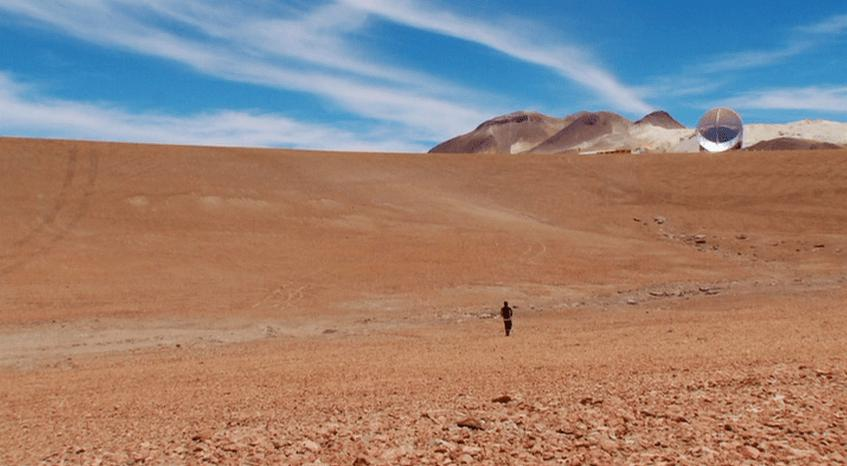
\includegraphics[width=85mm]{./imgs/chile.jpg}
\caption{\tiny{\Formular{{\slsc{Frame}} de {\slsc{Nostalgia de la Luz}}, filme de Patricio Guzmán}}}
\end{figure}


Outra forma de desaparecimento é aquela que ocorre, ainda hoje, em Pozo
Meléndez, no estado mexicano de Guerrero, ao sul de Acapulco. Trata"-se
de uma cratera de cerca de trinta metros de largura, e cuja profundidade
é desconhecida --- não se escuta nem sequer o barulho de uma pedra tocando
o solo, quando arremessada da superfície. Ali todo um regimento francês
teria sido empurrado buraco abaixo quando da invasão de Napoleão \versal{III} ao
México. Durante a \emph{guerra suja}, centenas de
militantes de esquerda foram ali jogados, assim como vítimas da guerra
contra o narcotráfico, mais recentemente.

Seria possível conceber essas formas de assassinato como o modelo por
excelência, a forma mais bem acabada da aniquilação e do extermínio. A
forma prototípica da \emph{cultura do terror}: mata"-se sem deixar vestígio do
crime, e se dissemina um sentimento de imprevisibilidade e
inexplicabilidade diante da violência e da morte, em que é impossível
saber quem a comete, e quem será o próximo a desaparecer. Como os
desaparecidos não necessariamente são membros dos grupos perseguidos,
trata"-se de um mecanismo no processo de transformação do medo em
terror generalizado. Aqui parece que estamos diante de um poder que se exerce pela
formação de vácuos, de vazios, em nada próximo à fórmula das sensações
dependente de gestos e imagens.

Entretanto, ao se tratar das formas de violência, inexiste uma que se
sobreponha à outra em términos de função e eficácia; cada uma cumpre
funções distintas. Nesse sentido, a disseminação de corpos mortos
mutilados, destroçados, desmembrados e decapitados, convertidos em
imagem de terror, não é oposta aos desaparecimentos. Ambas compõem, de
maneiras diversas, a \emph{cultura do terror}. Como coloca Pilar
Calveiro, ``sempre o poder mostra e esconde. E se revela tanto no que
exibe quanto no que oculta''.\footnote{Idem, p.~38.}

O medo, elevado a uma escala disseminada de terror, converte"-se em um verdadeiro
dispositivo de controle político e social, de algum modo em consonância
com os mais altos valores da sociedade. Competição,
individualismo extremo e uma guerra de todos, reivindicada como modelo no plano econômico, e que o excede: ``de fato, acredito que deve se
considerar as políticas de proliferação do medo como um dos dispositivos
característicos da governamentalidade neoliberal'',\footnote{\scalebox{.8}{BLANES}, Jaume
  Peris. ``Nuevas violencias, nuveas voces y nuevas resistencias en
  tiempos de reorganización hegemónica''. Entrevista a Pilar Calveiro.
  Avatares del Testimonio en América Latina. {\slsc{Kamchatka}}, 6 dez.
  2015, p.~884.} afirma Calveiro.

Tais formas de desaparecimento foram investigadas com sensibilidade pelo
cineasta chileno Patricio Guzmán em \emph{Nostalgia da luz} (2010) e
\emph{O botão de pérola} (2015). As duas obras tratam de incorporar em
sua própria forma fílmica esse vazio narrativo, sem recorrer à exposição
de corpos sem vida como forma de denúncia ou choque.


\asterisc

As relações entre as atuais situações de terror em países da América
Latina e aquelas que marcaram as ditaduras e repressão contra diversos movimentos de
esquerda são aquelas que marcaram mais pela continuidade do que pela ruptura. Vale a
pena tomar como exemplo o relatório da Comissão Nacional da Verdade
brasileira. Embora seja um documento sem precedentes na recente política
nacional, contém um buraco em suas páginas: reconhece que as práticas de
violência da Ditadura Civil"-Militar iniciadas em 1964 são herdeiras da
maneira como a polícia civil efetuava torturas e assassinatos de
delinquentes ``comuns'', mas não investiga como tais práticas cresceram
na ditadura diante do aumento das graves violações de direitos humanos,
enfocando"-se ``apenas'' em crimes cometidos contra militantes políticos.

Outra continuidade das violências que uma certa narrativa acredita fazer
parte do passado se entrevê na perpetuação do genocídio contra a
população negra e periférica pelas forças estatais, mediante a
justificativa da categoria ``resistência seguida de morte''. A categoria
foi amplamente questionada por diversas organizações de direitos humanos
diante dos indícios de que grande parte dos casos designados por esse
termo consistem em execuções sumárias, com tiros na cabeça, de pessoas
já rendidas. Tanto é que por recomendação da Secretaria Nacional de
Direitos Humanos da Presidência da República, o Governo do Estado de São
Paulo mudou a categoria para ``morte decorrente de intervenção
policial''. Mais recentemente, o Sérgio Moro, na figura de Ministro da Justiça, propõe o ``excludente de ilicitude'', que retira a responsabilidade penal de policiais que assassinarem pessoas, caso os primeiros tenham ``escusável medo, surpresa ou violenta emoção''.

Em diversos países da América Latina não se criou uma consciência
crítica em relação às formas de violência extrema, como pretendem países
como Alemanha, França e Itália, muitas vezes de maneira cínica, é
verdade, com relação ao nazifascismo. Pelo contrário, a violência
ditatorial em alguns países da América Latina é reivindicada com
orgulho, como em falas de que a ditadura ``salvou o país do comunismo'',
ou que ``o único erro que cometeram foi o de não exterminar a todos os
esquerdistas'', ou que salvaram o país de virar uma ``outra Cuba'', ou
mesmo o revisionismo mais tacanho, de equiparar torturadores a
militantes esquerdistas, afirmando que ambos cometeram excessos.

As atuais guerras contra os pobres, da qual a guerra contra o
narcotráfico é uma das facetas, criam uma identificação entre a imagem do violento com a
de ladrões e marginais. Aqueles que detêm o poder de grandes
organizações criminosas ou corruptas, que possuem relações íntimas com
grandes conglomerados empresariais e com o Estado não são vistos como perpetradores de violência. Estes últimos sequer se
encaixam no conceito de violência hoje em vigor, embora os danos e
mortes que causem sejam incomensuravelmente maiores daqueles tidos como
``criminosos comuns''. Inexiste, afinal de contas, um conceito de
violência que dê conta da violência sistêmica estruturante das
relações econômicas.

\asterisc

\emph{Fino fantasma} é uma performance realizada em São Paulo pelo
artista guatemalteco Naufus Ramírez"-Figueroa. O local da performance, a
Casa do Povo, é por si só significativo: monumento vivo criado em meados
dos anos 1950 em memória aos judeus mortos no nazismo. A performance
consiste em um ritual, com luzes dispersas pelo espaço, charutos, velas
e bacias com água. Muito pouco, ou quase nada, acontece em términos de
movimentação. Impera o silêncio. Embora não tivesse sido explicado,
alguns comentários antes do início afirmavam que se tratava de uma forma
de evocação dos mortos da ditadura guatemalteca, uma tentativa tímida,
sutil e pouco ruidosa de estabelecer um contato com eles.

O \emph{ritual} abre outro caminho para questionar as imagens violentas,
não exatamente na ordem do racional e do intelectual, e sim no plano do
sensível. A performance"-ritual desloca o eixo de equilíbrio centrado na
relação entre ocorrido e obra, para a relação obra"-ritual e
espectador"-participante. Um ritual que se desenvolve marcado por uma
dimensão temporal específica também, de recusa à passagem do tempo que
marcaria um antes e um depois, base de um discurso de superação definitiva da
violência e da marcha histórica da narrativa de progresso que a
acompanha. Tanto no caso dos dois filmes de Patricio Guzmán citados
acima, quanto no da performance"-ritual de Naufus, experimenta"-se um vazio
como crítica da continuidade da violência, nas antípodas da visualidade
e exposição de corpos destroçados como denúncia.

\asterisc

Para terminar, vale voltar às reflexões teológicas sobre a função da
imagem, de onde parti: a \emph{Incredulidade de São Tomás}, de
Caravaggio. A obra trata do famoso episódio em que o Apóstolo Tomás
questiona a ressurreição de Cristo, convidado por esse a tocá"-lo para
certificar"-se da sua realidade e então atestar o milagre. Caravaggio,
ao abrir uma fenda na vestimenta do braço esquerdo de São Tomás, parece
jogar com o próprio espectador, como se o instigasse ele mesmo a tocar São
Tomás e verificar a realidade da representação. Se era esperado que esse
tema clássico da pintura religiosa, além de auxiliar no ensinamento e na
memorização, provocasse a devoção e piedade, Caravaggio nos provoca a
antes de tudo desconfiar das imagens, e das funções que a elas são
atribuídas.

\begin{figure}[!ht]
\centering
 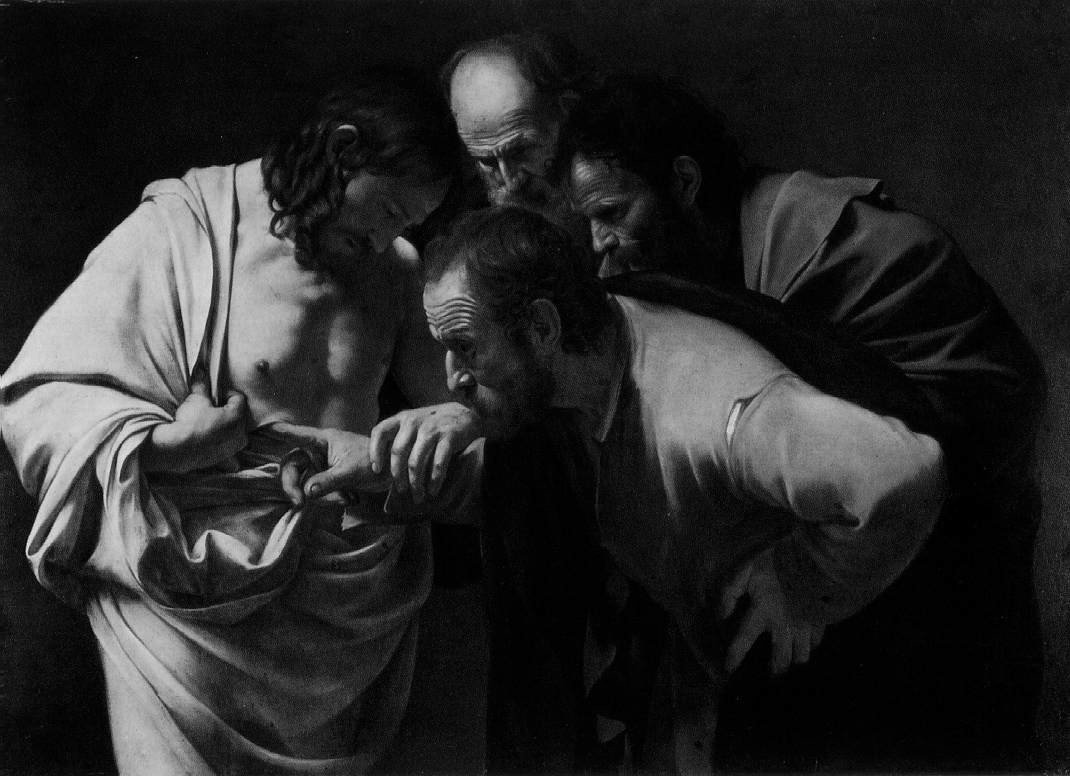
\includegraphics[width=85mm]{./imgs/crer.png}
\caption{\tiny{\Formular{{\slsc{A incredulidade de São Tomás}}, de Giovanni Caravaggio}}}
\end{figure}

\chapter*{Vozes da Amazônia\footnote[*]{Este ensaio foi %mudar para asterisco
  previamente publicado no site da {\slsc{Agência de Jornalismo Amazônia Real.}}}}
\addcontentsline{toc}{chapter}{Vozes da Amazônia}

``A gente tem uma história. Mas se a gente contar essa história pro
branco, eu falo assim, com certeza mesmo, o branco não vai confiar. A
gente tem uma história sim, mas se eu contar, você não acreditaria.
Então\ldots{} é difícil para mim''. Foi com essa frase que Yanuke Waurá,
indígena do povo Waurá, encerrou a entrevista que realizei com ela
durante o Acampamento Terra Livre, em abril de 2018, momento em que
diversos povos indígenas de todo o Brasil se encontram em Brasília para
discutir estratégias de lutas por direitos direito, como acesso aos seus
territórios tradicionais e por suas formas de vida.

Durante a entrevista, Yanuke contou sobre os impactos do agronegócio na
vida de sua aldeia. Ela vive no Parque Indígena do Xingu, localizado
no Estado do Mato Grosso --- o território foi o primeiro a ser homologado
no Brasil, em 1961, e por isso é de certo modo um ícone na luta dos
povos indígenas pelo seu direito de autodeterminação. A aldeia de Yanuke
fica nas proximidades do lago Piyulaga, que em português significa
``lugar de pesca''. Apesar do nome, o local se tornou inapropriado para
pegar peixes: ``na época de chuva, quando o rio vai enchendo, os
fazendeiros plantam a lavoura e jogam veneno. Como é época de chuva,
desce o rio e mata todos os peixes. Aí eu vejo peixe boiando. (\ldots{}) aí
começamos a falar: `a gente não pode comer esse peixe'", conta a
indígena, que participa intensamente do movimento político de mulheres
em sua aldeia. Elas passaram a tomar decisões junto aos homens sobre os
rumos da política local.

A área demarcada de seu território e as florestas que o circundam não
são suficientes para barrar os impactos do agronegócio.
As plantações de soja estrangulam o Território Indígena do
Xingu --- como preferem chamá"-lo os indígenas, recusando a associação
entre parque e jardim zoológico, embutida no nome oficial de Parque
Indígena do Xingu. Por motivos cosmológicos, diversos povos indígenas do Alto Xingu
não comem carne de caça (como veados, porcos do mato ou aves), diferente
dos hábitos alimentares de outros povos indígenas da América do
Sul. Isso implica que a ausência de peixes na alimentação,
principalmente das crianças, gera um sem"-número de problemas para essas populações.

A fala de Yanuke que encerrou a nossa entrevista veio como resposta a
uma pergunta que havia lhe feito, a respeito da história da origem de
seu povo e como eles concebem a origem do mundo em que vivem. Eu
acreditava poder dar um tom afetivo e sensível para a história de
violência e de resistência que escutava, e assim tornar o texto mais
complexo, ao tentar apresentar, ainda que de maneira pontual, traços da
riqueza e complexidade que marcam a visão de mundo de seu povo.

Mas a negação, ou melhor, a esquiva de Yanuke em responder a minha
pergunta, hoje me parece uma atitude muito mais profunda do que pude
compreender na época. Era a instauração de um limite, de uma separação:
``existem coisas que eu posso falar, que eu posso contar, mas que vocês,
brancos, não vão acreditar'', parecia dizer. ``Existe um outro mundo, no
qual eu vivo, e que é inacessível para vocês, pois vocês não
acreditam''. Ou pior, ``vocês o estão destruindo''.

\asterisc

Entrevistei Yanuke e mais cerca de quinze indígenas da Amazônia
brasileira enquanto estava fazendo a cobertura jornalística do
Acampamento Terra Livre para a agência de jornalismo investigativo
\emph{Amazônia Real}, com sede em Manaus. Provavelmente a única agência de
notícias localizada na Amazônia brasileira sem laços com famílias
historicamente proprietárias de terras e meios de comunicação. Estava
então acompanhado de um fotógrafo indígena, Yanahin Matala Waurá, primo
de Yanuke.

O clima durante o acampamento em 2018 era de tensão, e a conjuntura
política desfavorável para os povos indígenas. Após destituir a
presidenta Dilma Rousseff de seu cargo em um processo de impeachment com
poucas, se é que alguma, prova de crime de responsabilidade cometido
pela mandatária, o governo de Michel Temer estabeleceu uma relação
umbilical com os congressistas próximos ao agronegócio. Temer se
sustentava na força política mais abertamente anti"-indígena do país para
terminar o seu mandato, e evitar o seu próprio impeachment. Por isso,
diversas medidas de seu governo foram tomadas para agradar esse poderoso
bloco no Congresso, conhecido como Bancada Ruralista, e formalmente
organizados na Frente Parlamentar da Agricultura (\versal{FPA}).

Entre as decisões do executivo que no momento ameaçavam os povos indígenas estava a paralisação dos processos de
demarcação de terras indígenas, a locação de cargos da Fundação Nacional
do Índio (Funai) a pessoas afins aos grupos
evangelizadores, a proposta de lei de flexibilização do uso de
agrotóxicos (muitos proibidos em outros países) e a tentativa de
instaurar a controversa tese do marco temporal na judicialização de
processos de demarcação de terras indígenas.

A tese do marco temporal, defendida por ruralistas, define que os povos
indígenas localizados no Brasil teriam apenas direito às terras em que
se encontravam em 1988, quando da promulgação da Constituição
Brasileira. Um dos principais problemas envolvidos nessa tese é o
apagamento da história de violência a que foram submetidos os povos
indígenas, principalmente durante o período da Ditadura Civil"-Militar
(1964-1985). Ao longo desse período era comum os militares transportarem povos inteiros
de uma região à outra, independente de sua vontade e conforme o
interesse dos projetos de construções de estradas e ocupação por
produtores rurais.

Difícil de calcular, estima"-se que 8,3 mil indígenas foram mortos
durante a Ditadura Civil"-Militar. Esse número, definido pelo relatório da
Comissão Nacional da Verdade, criada durante o governo Dilma Rousseff
para apurar os crimes cometidos pelos militares durante a ditadura, não
leva em conta, por exemplo, o relatório da Cruz Vermelha sobre os crimes
contra indígenas durante a ditadura, produzido entre o final dos anos 1960
e início dos anos 1970, e que veio a público apenas em 2016 --- ou seja, após a publicação do Relatório da Comissão da Verdade.

Outro fator de tensão era a força que ganhava Jair Bolsonaro para a
corrida presidencial. Em abril de 2017, um ano antes, Bolsonaro afirmou,
em palestra no Rio de Janeiro, que no seu governo ``não vai ter um
centímetro demarcado para reserva indígena ou para quilombola''. Nas
primeiras horas de governo, assim que tomou posse, em janeiro de 2019,
Bolsonaro deslocou para o Ministério da Agricultura as duas principais
atribuições da Funai: demarcação de terras indígenas e quilombolas e o
processo de licenciamento para empreendimentos que possam atingir esses
povos. Chefiado por uma das líderes do setor agropecuário, a deputada
federal Tereza Cristina, o Ministério da Agricultura é o principal
interessado em representar o setor ruralista, contrário aos processos
de demarcação, e que considera que os povos indígenas e os direitos a
eles associados impedem o produtor rural de trabalhar.

\asterisc

Ao longo dos últimos anos, tenho realizado uma intensa cobertura
jornalística da Amazônia. Com cerca de 5.846.100 km², trata"-se da maior
bacia hidrográfica e maior floresta do planeta, abrangendo nove países:
Bolívia, Peru, Colômbia, Equador, Venezuela, Guiana, Suriname, Guiana
Francesa e Brasil. Narrar os conflitos políticos que ocorrem em um
território tão vasto implica desafios consideráveis, tanto pela
amplitude da área como pela dificuldade de acesso a zonas remotas,
custos envolvidos, perigos naturais e possibilidade de desentendimentos
com madeireiros, garimpeiros e fazendeiros --- que em mais de um caso
implicou na morte de jornalistas. A região, rica em petróleo, minérios,
com elevado potencial hidrelétrico e de produção de grãos
(principalmente soja), pode ser considerada como uma das fronteiras em
expansão do capitalismo contemporâneo.

A minha decisão de cobrir estes conflito tem implicado em ``escrever de
perto'' a essas populações amazônicas, como propõe a artista e teórica
vietnamita Trinh T. Minh"-ha. Evitar falar sobre e evitar elaborar
explicações e análises; trata"-se menos de formular uma gramática dos
conflitos e mais uma tentativa de explorar e reverberar os enunciados de
pessoas cujas trajetórias de vida se confundem com a da transformação
violenta de seus territórios. Seja em meu trabalho como antropólogo,
seja em meu trabalho como jornalista, o desafio é recontar as histórias
de destruição da floresta e do território amazônico ressoando a
narrativa das pessoas mais afetadas por esses processos:
populações indígenas, ribeirinhas e quilombolas.

Nesse ensaio, faço uma compilação desses enunciados sobre a violência e
destruição de formas de vida, bem como das resistências. Se tais relatos, à primeira vista,
podem parecer similares e repetitivos, se a recorrência de formas de
destruição permitiriam identificar uma gramática bem delimitada da
forma como tais conflitos ocorrem, talvez valha a pena explorar um outro
caminho, que a fala de Yanuke nos abre. Não o que todos esses relatos
dizem de parecido, mas o equívoco profundo envolvido no contato entre
mundos diversos.

Como coloca o antropólogo Eduardo Viveiros de Castro, a antropologia tem
o desafio de traduzir outras formas de conceber o mundo, para além de
nossas projeções etnocêntricas sobre o outro: a antropologia como uma
forma de conhecer como outros povos conhecem o mundo, a antropologia
convertida em meta"-antropologia. O equívoco, assim, não seria um erro,
uma falha na tradução ou na comunicação; inexiste uma tradução correta,
por não existir um referencial único a ser traduzido de maneira
inequívoca.

Existe algo que excede à possibilidade de tradução de mundos. Explorar o
equívoco permite entender que o mesmo termo, a mesma forma de falar,
implica coisas distintas para o indígena que o enuncia e para o não indígena que
o escuta. A escuta do outro, o escrever de perto, pode ensejar essa
forma de equívoco no próprio texto, adentrando as bases a partir das
quais tais equívocos ocorrem. Tentar explicitar as fissuras e os
incomensuráveis implicados na comunicação, onde acreditávamos estar a
potência do diálogo, da compreensão mútua e da possibilidade de um
mundo.

São essas vozes, e esses equívocos, que procuro trazer neste ensaio.

\asterisc

Domingos Peas é um líder político Achuar que conheci enquanto trabalhava
na cobertura do Fórum Social Panamazônico, em abril de 2016, em
Tarapoto, na Amazônia andina do Peru. Os Achuar vivem na fronteira entre
Peru e Equador, ``nós, indígenas, nunca tivemos fronteiras. Por isso
temos conversado muito aqui sobre como rompê"-las'', conta Peas.

Sua vinda para o encontro que reunia populações dos nove países que
compõem a bacia amazônica estava vinculada à criação de um parque
binacional de preservação das nascentes do Rio Amazonas, projeto que
leva o nome de \emph{As Bacias do Rio Napo e do Rio Marañón}: ``esse
projeto, para mim, é a única possibilidade que resta em nossas mãos''. A
fala de Peas e seu uso da língua espanhola, na qual nos comunicávamos e
que não era a primeira língua de nenhum de nós, misturava um tom
profético e de certeza. Peas repetia expressões que ouvi com pouca
frequência em espanhol, apesar de ter viajado por e residido em diversos
países de língua espanhola.

``Ustedes sabrán'' (``vocês saberão'', em português) talvez seja a
mais utilizada e aquela com que melhor consigo expressar a
sensação de que não era uma entrevista qualquer, mas que me
encontrava diante de um discurso profético, de que havia uma mensagem
que demandava ser proferida e escutada, que Peas dirigia ao fundo dos
meus olhos, sem desviar o seu olhar, em nenhum momento de quase uma hora de conversa. ``Vocês saberão que a selva da
qual nós cuidamos não foi criada para finalidades monetárias, mas porque
temos uma conexão com nossa \emph{madre tierra}''. ``Vocês saberão que
antes as fronteiras não existiam para os indígenas. São os interesses da
colonização que legitimaram que cada Estado criasse as suas fronteiras,
para desenvolverem os seus projetos de exploração e interesses
alheios''.

Em sua argumentação, Peas analisa o impacto que as ações de povos
não indígenas tem sobre o seu território, sobrepondo um discurso que
incorpora análises geopolíticas e científicas, bem como a importância
dos Achuar e demais povos indígenas do mundo: ``todos nós
sabemos que os diferentes problemas que afligem a Amazônia não são
produzidos por nós, mas sim por empresas multinacionais. Não os estamos
criando nós, mas eles, os países industrializados, que poluem, não
reduzem suas emissões de poluição, seguem contaminando, e ainda por cima
vêm destruir o nosso território. Por isso essa posição de conservar,
pois essas serras têm uma função essencial no acúmulo das águas que
servem todo o continente. É necessário, se não queremos ter uma
destruição irreversível, manter, cuidar desta selva'', afirma Peas,
mantendo o seu tom profético.

O líder Achuar questiona cientificamente qual dos projetos é o mais
viável, como que desafiando o conhecimento que temos do
mundo: ``o projeto também consiste em deixar de lado tudo o que se
refere às mineradoras, pois sabemos que por melhor que seja a
tecnologia, sempre haverá poluição. Por isso temos que analisar,
comparar, tecnicamente, cientificamente, economicamente. Analisar as
opções: que desenvolvimento deu o petróleo? E se preservarmos essa
floresta, que desenvolvimento teremos? Temos que comparar. Não falar
assim por falar, mas falar tecnicamente, com fundamentos, com
argumentos''. Sua fala é calma, pausada e firme. Ele apresenta a sua
alternativa, baseada nos modos de vida indígena, como a mais certeira,
tanto para não indígenas quanto para indígenas: ``daí nossa missão em
conservar essas bacias sagradas, com nossas culturas, nossos ritos,
nossos idiomas. Com nossas formas de administração da selva''.

\asterisc

Um dos planos mirabolantes que os militares que governaram o Brasil
durante mais de vinte anos elaboraram para a Amazônia era torná"-la um
grande lago navegável, para a defesa do território brasileiro, conforme
conta o jornalista Rubens Valente na obra \emph{Os fuzis e as flechas}.
Em seu livro, investiga as violências cometidas pelos militares contra os povos
indígenas, a partir de minuciosa pesquisa em arquivos. Essa imagem,
inundar a Amazônia para torná"-la um grande lago navegável, torna"-se
potente para pensar a Amazônia hoje, justamente por misturar delírio e
realidade. Traz à mente imagens como aquelas eternizadas no cinema por
Werner Herzog, que recria a história do irlandês Brian Sweeney
Fitzgerald, o Fitzcarraldo, que dá nome ao filme, um dos barões do ciclo da borracha, em
êxtase, ensandecido por um projeto de transportar uma ópera rio acima,
até Iquitos, no coração da Amazônia peruana, custe o que custar.

Como devaneio que é, essa imagem permite um ponto de vista privilegiado
para aproximar"-se dos mega"-projetos que hoje destroem o território
amazônico, e que ressoa no imaginário dos militares
brasileiros durante a ditadura. ``Um deserto verde'', diziam, ao
referir"-se à Amazônia, acreditando, ou talvez desejosos de fazer
acreditar que se tratava de um território em que inexistiam pessoas.
Toda uma região para a qual queriam fazer emigrar massas de
trabalhadores sem"-terra, do Sul do país e da região Nordeste,
retirando"-os da seca com promessas fáceis ou com o objetivo de diminuir
a força de movimentos de esquerda ligados ao campo e em nome da reforma
agrária, como as Ligas Camponesas. Surgidas em 1946 e ligadas ao Partido
Comunista do Brasil, as Ligas foram duramente perseguidas durante o
período ditatorial.

A ideia de alagar a Amazônia, tão absurda como imagem que chega a parecer inimaginável, diz algo a respeito de projetos que, para se tornarem
reais, envolveram grande destruição e custaram a vida de milhares de
pessoas. Entre essas obras insanas encontra"-se o empreendimento de
construção da Estrada de Ferro Madeira"-Mamoré, cruzando o estado de
Rondônia, que após duas tentativas frustradas de ser construída no
século \versal{XIX}, foi concretizada pelo empreendedor norte"-americano Percival
Farquhar entre 1907 e 1912, causando a morte de cerca de 6 mil
trabalhadores, acometidos por disenteria, malária e outras doenças
tropicais. Ou o projeto iniciado em 1927 por Henry Ford, em Belterra
e Fordlândia, às margens do Rio Tapajós, no oeste do Pará, para suprir com látex suas fábricas de pneus, e que faliu,
já que nenhum dos gerentes do empreendimento tinha conhecimento de
técnicas de plantio nos trópicos, dispondo as seringueiras (árvore da
qual se origina o látex), muito mais próximas umas das outras do que
usualmente se encontram na selva, tornando"-as alvo fácil para as pragas
que vieram a devastá"-las. Também a construção das três grandes rodovias
que visavam ``integrar'' a Amazônia ao território nacional e desenvolver a
região fazem parte dessa série de projetos que se sobrepõem de maneira
violenta aos mundos pré"-existentes a eles, como a Transamazônica, a
Perimetral Norte e a Cuiabá"-Santarém. Todas de difícil construção,
implicaram na morte de milhares de trabalhadores e a devastação dos
povos indígenas locais e da natureza.

Cada uma dessas obras traz em si um pouco do projeto de alagamento da
Amazônia para proteção das fronteiras brasileiras, na medida em que
todas são projetadas e construídas sem levar em consideração as pessoas
que vivem nesses territórios. Cada novo ciclo de desenvolvimento na
Amazônia vem acompanhado de novas formas de destruição. Entre as mais
recentes, estão os projetos de construção de usinas hidrelétricas.
Apenas para a Amazônia brasileira, estima"-se que serão
construídas cerca de cem usinas hidrelétricas nos próximos anos, e cerca
de 250 em toda América Latina.

Patricia Juruna tinha 27 anos quando a entrevistei durante o Acampamento
Terra Livre de 2018. Filha de uma indígena Juruna com um pai branco,
Patricia não cresceu na aldeia de seu povo, localizada nas imediações da
volta grande do Xingu, onde foi construída a Usina de Belo Monte, uma
das mais controversas obras de infraestrutura projetadas durante os
governos do Partido dos Trabalhadores. Em sua adolescência, sempre que
possível Patricia visitava a aldeia de origem de sua mãe. Nessas
visitas, uma de suas tias lhe contava as histórias de seu povo: ``ela
que foi me transmitindo tudo o que eu não tive em minha infância, que as
pessoas tiveram na aldeia e eu não''. Patricia conta que sua bisavó
também se casou com um não indígena. Seu povo tinha muitos conflitos com
os vizinhos Kayapó. Um dia, há muito tempo, invadiram sua
aldeia para raptar as mulheres e matar os homens. Sua avó fugiu para a
mata, para escapar, e acabou no acampamento de seringueiros onde
conheceu Plácido, seu futuro esposo. Após a morte de Plácido, casou com
um indígena de outro povo, os Arara.

Hoje moradora da cidade de Santarém, local onde se encontram as águas
dos Rios Tapajós e Amazonas, Patricia é uma militante contra a
construção das usinas hidrelétricas previstas na bacia do Tapajós --- tendo
em mente o que aconteceu com a construção de Belo
Monte: ``o governo vem com esse discurso que a hidrelétrica é
sustentável\ldots{} eu fico tão indignada com isso, porque não é
sustentável nem do ponto de vista ambiental nem social. Aquelas pessoas
tinham o seu modo de vida, que não foi respeitado. Elas viviam a vida
toda ali, e de repente tiveram que sair'', conta Patricia.

``Elas não tiveram opção: era sair ou sair. Diziam `você tem até tal
data pra sair!'. A gente, por exemplo, não pode chegar em um cemitério
dos brancos, que para vocês é sagrado, e colocar a nossa aldeia lá em
cima, e sair quebrando tudo. E por que os não indígenas podem fazer isso
com a nossa terra?'', questiona Patricia Juruna, que hoje se dedica também ao
fortalecimento da rede de mulheres indígenas do Baixo Tapajós, com a
organização de encontros e eventos de troca de formas de cuidado
tradicionais e empoderamento das mulheres.

No Rio Tapajós, toda a devastação causada pela construção de Belo Monte
serve como um espelho aterrorizante diante do que pode se passar com os
territórios localizados às suas margens. Belo Monte foi amplamente
questionada por ambientalistas e por técnicos do sistema de
abastecimento de energia no país. Estima"-se que o elevado custo desta obra
faraônica e os impactos socioambientais irreversíveis por ela gerados
possam sair mais caros do que o seu potencial energético. Além disso, a
cidade de Altamira dobrou a sua população em cinco anos, recebendo
grande parte das comunidades indígenas e ribeirinhas desalojadas pela
construção da usina. Em 2018, Altamira foi considerada a 8ª cidade mais
violenta do país, com cerca de 91,9 homicídios para cada 100 mil
habitantes.

Ao testar a sua primeira turbina, em 17 de fevereiro de 2016, um
incidente gerou a inundação do principal reservatório da barragem. Mais
de 16 toneladas de peixes foram encontrados mortos, o que ocasionou
também a morte de um sem número de aves. Apesar da multa milionária
aplicada pelos órgãos de fiscalização ambiental brasileiros, a empresa
responsável pelo consórcio segue sem cumprir as medidas de compensação,
como construção de uma infraestrutura mínima aos desalojados. O
documentário \emph{Belo Monte: depois da inundação}, do cineasta canadense Todd
Southgate, que pode ser encontrado on"-line, dá uma dimensão da tragédia.
Na esteira da construção da hidrelétrica, o projeto da Belo Sun Mining,
empresa de origem canadense, está às voltas com a legislação brasileira
para começar a extração de ouro nas imediações da Volta Grande do Xingu.

Por isso a pressa e o desespero do povo indígena Munduruku em ter parte
de seu território demarcado, nas margens do Rio Tapajós. A Terra
Indígena Sawré Muybu possui 178.173 hectares, e desde abril de 2016 é
reconhecida pelo governo brasileiro como território indígena,
mas ainda não foi homologada pelo poder executivo. Como forma de
pressionar o governo brasileiro, os indígenas Munduruku, com apoio da
\versal{ONG} Greenpeace, realizaram o mapeamento do seu próprio
território, o ``Mapa da vida: a visão do povo Munduruku sobre seu rio e
seu território'' (disponível on"-line), que indica lugares sagrados e seus
conhecimentos ancestrais sobre a natureza da região. Hoje, o território
Munduruku é ameaçado por garimpeiros ilegais, madeireiros e pela
construção de cerca de 42 usinas hidrelétricas na Bacia do Rio Tapajós,
cujos efeitos, à imagem de Belo Monte, podem ser devastadores. A
contaminação por mercúrio no Tapajós, que tem origem tanto no garimpo
ilegal quanto na construção de hidrelétricas --- já que coloca em circulação
camadas subterrâneas de mercúrio --- se transformou em um grave
problema de saúde na região.

\asterisc

Outros países da América do Sul passam por processos similares, com suas
devidas particularidades. José Antonio Saldarriaga Tabares
me contou sobre a resistência contra a exploração de minérios e petróleo
no território tradicional de Caquetá, na Colômbia. Emerald Energy, uma empresa
chinesa, ``pretendia explorar petróleo e outros minérios. Mas nós nos
colocamos durante dois meses bloqueando uma ponte de passagem
obrigatória. Nos expulsaram a balas. Tivemos quinze feridos, dois com
extrema gravidade, um dos quais já não é mais o mesmo'', conta. José
Antonio entrou em greve de fome, enquanto a comunidade à qual pertence
protestava contra o exército e a polícia; estes tratavam, sem sucesso,
de garantir a ordem para que os estudos de prospecção da mineradora
chinesa ocorressem. Apesar da Suprema Corte da Colômbia ter decidido que
as comunidades devem ser consultadas quanto aos projetos que o governo
deseja desenvolver em seus territórios, os prefeitos e governadores da
Colômbia não aceitam tal decisão, que já foi levada para organismos
internacionais arbitrarem.

José Antonio é também cético quanto ao processo de paz firmado entre o
governo colombiano do presidente Juan Manuel Santos e as Fuerzas Armadas Revolucionarias de Colombia --- Ejército del Pueblo (\versal{FARC}-\versal{EP}), em 2016:
``opino, de maneira muito pessoal, que essa `paz' que está criada
tem também como fundo permitir que entrem mega"-projetos extrativistas
antes impossíveis. Pois quando estava a guerrilha, as multinacionais não
entravam em todas as partes, pois tinham medo. E isso eu vejo com muito
pessimismo. Aplaudo o processo de paz, pois um morto a menos já é um
grande ganho. Mas não acredito que estejamos construindo as bases para
que essa paz seja sólida e duradoura''.

Nossa conversa foi realizada em 2017, portanto, cerca de um ano após a
assinatura dos acordos de paz com as \versal{FARC}. Em 2018, o fenômeno de
``asesinato de líderes sociales'', como passou a ser chamado na
Colômbia, atingiu níveis alarmantes: entre 1º de
janeiro de 2016 e 30 de novembro de 2018, estima"-se que 423 líderes
sociais tenham sido assassinados. Muitos deles eram líderes de
associações comunais, a principal forma de gestão de territórios em
zonas afastadas. Esses assassinatos, para muitos analistas, minam as
bases dos acordos de paz.

Equador e Bolívia são dois países que compõem a região amazônica e que
no final da primeira década do século \versal{XXI} animaram ambientalistas e
defensores de direitos humanos por todo o mundo. Na Bolívia, o que mais
chamou a atenção foi o processo de elaboração da Constituição pelo
governo de Evo Morales, que culminou na redefinição da Bolívia como um
Estado Plurinacional, e estabeleceu direitos inéditos aos povos
indígenas na gestão de seus territórios e participação no governo. Já no
caso equatoriano, foi durante o governo de Rafael Correa que se
estabeleceram os direitos da Natureza (\emph{Pachamama}) na Constituição
de 2008. Ou seja, o reconhecimento da natureza enquanto
sujeito de direito.

Em ambos os Estados vinham predominando governos de
centro"-esquerda, marcados por um forte discurso ambientalista e uma
relação de afinidade com os movimentos indígenas. Entretanto, o que
narram pessoas desses países difere muito da imagem com a qual se
promoveram os Estados boliviano e equatoriano.

Gabriela B. (a militante preferiu ocultar seu sobrenome com receio de
perseguições, o que dá uma ideia do ambiente), é originária de
Quito, no Equador. Formada em Ciências Sociais, tem trabalhado junto a
populações indígenas de seu país. ``A verdade é que o extrativismo se
intensificou como nunca nesses últimos anos. A renegociação dos
contratos petroleiros permitiu que o Estado aumentasse, e muito, a sua
parte. Pois antes os ganhos eram insignificantes. E isso também permitiu
ao Estado entrar em outras lógicas mais, digamos, `gananciosas'. Um
caso hoje emblemático é o da comunidade indígena Shuar de Nankint, na
Cordilheira do Cóndor. O projeto Cóndor Mirador, empreitada chinesa, é
um dos maiores projetos de mineradoras do país. A análise de impacto
ambiental realizada pela empresa mostra que o Rio Tundaíme, um rio vivo
e despoluído, será desviado. No leito deste rio vão colocar todos os
detritos das mineradoras, uma barragem como aquela que se rompeu no
Brasil, só que nove vezes maior'', diz a cientista equatoriana,
comparando o caso do Rio Tundaíme com o da barragem da empresa Samarco,
que se rompeu em Mariana. Na primeira versão deste ensaio, o ocorrido em Mariana era considerada a maior tragédia ambiental do país; de lá para cá, tivemos também Brumadinho, que torna qualquer competição pelo ``pior'' irrelevante e assombrosa.

Para Gabriela, o governo de Rafael Correa começou com um discurso e
práticas muito interessantes. Mas de certo modo, o processo da
estabilização da economia e das demandas políticas da sociedade
equatoriana abriu caminho para o incremento de mega"-projetos
extrativistas em áreas sensíveis como o Parque Yasuní, uma das reservas
mais importantes do Equador, no qual o governo Correa permitiu a entrada
de mineradoras e petroleiras.

Processo similar ocorreu na Bolívia de Evo Morales, em que o próprio
governo manteve um discurso ambientalista e pró"-indígena por um lado, e,
por outro, foi um grande aliado dos fazendeiros que desmatam a Amazônia
para pecuária ou para plantar soja, sorgo, arroz e trigo, e de mega"-projetos extrativistas. ``Nos últimos três, cinco anos, o governo tem
estado cada vez mais próximo ao agronegócio'', diz a militante G.~C.,
que preferiu manter o anonimato, com receio de represálias em seu país.
Para ela, um dos resultados da aproximação do governo aos movimentos
indígenas é que o país ficou sem lideranças indígenas para lutar contra
as decisões do governo. ``Quando olhamos para os governos de esquerda
que tivemos pela América Latina, vemos que tivemos muitos retrocessos no
tocante aos direitos humanos, não só na Bolívia. E isso é algo muito
difícil. Durante as ditaduras, sabíamos bem quem eram nossos inimigos, e
como deveríamos atuar para que não nos matassem nem fisicamente, nem
civilmente. Agora já não sabemos mais como enfrentar esses inimigos,
pois são de esquerda, são democráticos, e além de tudo falam da
pluralidade''. Nesse momento o olhar de G.~C. fica visivelmente mais
apreensivo e preocupado.

Observação: desde que escrevi este ensaio até o momento de sua publicação, muita coisa aconteceu. Evo Morales sofreu um golpe após um processo eleitoral conturbado, Rafael Correa está exilado na Bélgica, com mandado de prisão expedido pela justiça equatoriana, e Bolsonaro implementa uma verdadeira guerra de destruição contra a floresta e seus defensores. Ao pensar na experiência de centro"-esquerda que governou a América Latina no início do século \versal{XXI}, me pergunto que legado deixaram, no que diz respeito às formas de lidar com a floresta e seus povos. O debate é complexo, e como bom debate, não tem uma resposta única. Tenho a sensação de que é urgente, aliás, não apenas para uma posição ecossocialista, mas para todo campo político não interessado em repetir os erros do nacional"-desenvolvimentismo.

\asterisc

Gabriela B. compreende o atual processo de destruição da Amazônia sob o
avanço do capitalismo extrativista a partir da lógica de diferentes
economias em choque: ``nesse sentido é uma fronteira, política e
econômica. Neste embate, encontram"-se duas economias distintas, as
economias que fazem os povos indígenas, os povos amazônicos, que são
economias baseadas em outras cosmovisões: o compartir, o dar, a relação
com a natureza, a reciprocidade. E por outro lado, a economia
capitalista, com toda a sua lógica de acumulação do capital, de
desapropriação, de destruição e exploração dos territórios''.

Para a antropóloga sino"-americana Anna Tsing, que realizou toda uma
conceitualização da lógica embutida na expansão das fronteiras do
capitalismo, ao tratar do desmatamento na Indonésia: ``as fronteiras são desregulamentadas, porque surgem nos interstícios das colaborações entre parceiros legítimos e ilegítimos: exércitos e bandidos; gângsteres e corporações; construtores e desapropriadores. Eles confundem os limites da lei e do roubo, governança e  violência, uso e destruição. Essas confusões mudam as regras e, assim, possibilitam novas economias extravagantes de lucro, assim como perdas''. %%%indicar nossa trad? uma vez que não traz a referência...
Uma perspectiva
teórica afinada com a visão do líder colombiano José Antonio Saldarriaga
Tabares: ``temos que abrir os olhos, pois esse modelo extrativista nos
leva à ruína, nos traz apenas desigualdades sociais, contamina nossas
fontes hídricas, e sem água não há vida. Para ninguém''.

O capitalismo extrativista resguarda à Amazônia o lugar usual ocupado
por territórios do Sul na divisão colonial: o de fornecedor de matéria
prima, de mão de obra barata, de terra e de vidas. Mas a destruição das
formas de vida humanas e não humanas do território amazônico pode ter um
efeito devastador e irreversível para todo o planeta, como afirmam tanto
cientistas como xamãs indígenas (para os quais, evidentemente, o fim
da floresta possui significados muito distintos). Trata"-se de ``um dos
territórios mais afetados pelo delírio contemporâneo'', como bem colocou
Martina di Stefano, amiga e filósofa italiana a quem compartilhava algumas ideias e
receios em meu trabalho de pesquisa e cobertura jornalística.

\asterisc

Tenho escutado quatro temas aparecerem com frequência na forma como indígenas relatam os
conflitos políticos pelos quais passam: a destruição de seus territórios, a relação entre formas de alimentação e doenças, a importância das mulheres indígenas
nos processos de decisão política e a negação da identidade étnica de
indígenas.

Diferentemente dos modelos modernos de corporalidade, de maneira
genérica, pode"-se dizer que o corpo, para diversos povos indígenas, passa por um
incessante processo de feitura ao longo da vida, no qual a alimentação,
o comer aquilo que cada povo considera como comida de verdade, é
central. Comer comida ruim, ``comida de branco'', é muitas vezes associado a
doenças. Em diversas ocasiões escutei de indígenas que os problemas de
saúde enfrentados hoje por essas populações inexistiam no tempo dos
antigos.

``Muitos jovens vão às cidades com cânceres que até pouco nós não
conhecíamos'', afirma a liderança Achuar Domingos Peas, na mesma
entrevista em que falamos sobre o seu projeto de parque para a proteção
das nascentes do Rio Amazonas. Para Margarita Rodriguez Weweli"-Lukana, do
povo Sikuani, que vive na fronteira entre a Amazônia colombiana e
venezuelana, ``nossos avós viveram muitos anos. Naquela época, não tinha
poluição nem contaminação, não sofriam de parasitas, nem de gastrites,
nem de apendicite, nem de problemas de cólon, não sofriam de hepatite,
nem de nervos, nem de más formações\ldots{} mas agora com a comida que
leva muitos produtos químicos, temos todos esses problemas'', afirma
ela.

Margarita me contou também que sua avó havia participado da grande
guerra mundial. Espantado, perguntei como isso era possível, e a que
guerra ela se referia, imaginando estar aludindo à Primeira ou à Segunda
Guerra Mundial que ocorreram majoritariamente em solo europeu.
Constrangido, ouvi a sua resposta: ``a colonização, a grande guerra''.
Pouparam a sua avó, mas mataram a irmã dela: ``cortaram os braços,
abriram o seu tronco, e em uma forma redonda, fizeram com que as outras
guerreiras observassem como batia o seu coração, com ela viva, toda
aberta''.

Um dos movimentos reivindicatórios mais fortes na região amazônica é o
de mulheres. Rosimere Arapaso, que entrevistei durante um
protesto em Brasília em 2018 contra a utilização do marco temporal em
processos judiciais, é originária do Alto Rio Negro e participa da
Makira"-Etê, rede de mulheres indígenas do estado do Amazonas. ``São as
mulheres que estão na linha de frente, e que sofrem muitas ameaças hoje.
São elas que estão lutando pela defesa de seus territórios, pois seus
maridos estão mortos, seus filhos guerreiros estão sendo mortos ou estão
mortos. Então só sobraram as mulheres indígenas na linha de frente de
guerra, e é por isso que estamos com a voz das mulheres indígenas: `nós
pedimos respeito!'".

``Enquanto mulheres, temos que lutar conjuntamente com os homens, diante
das inúmeras ameaças que nos rondam. Mas também temos nossas
particularidades, pois nós também queremos decidir nos manifestar a
respeito de outras problemáticas. E uma delas é justamente a
participação das mulheres dentro das próprias comunidades, pois muitas
vezes não somos consideradas como qualificadas'', afirma Ketty Marcelo
Lopez, indígena Ashaninka e presidenta da Organização Nacional de
Mulheres Indígenas Andinas e Amazônicas do Peru. Ketty reivindica a
participação das mulheres em todos os âmbitos decisórios da vida
comunitária indígena e nos cargos diretivos. É comum ouvir também de
mulheres indígenas acerca do papel diferencial que possuem as mulheres
em relação aos homens na formação das comunidades, por sua relação mais
forte com a terra.

Como todas as sociedades, as sociedades indígenas não se encontram
paradas no tempo, ou mesmo fora da história. A ideia de que essas
sociedades estariam se ``falsificando'', ou perdendo a sua
``originalidade'' ao incorporarem objetos, tecnologias e reflexões de
outras culturas, depende de uma visão colonialista de que a história
desses povos teria se iniciado na colonização, de que antes não se
transformavam. Pelo contrário, a incorporação de objetos como motores
elétricos, por exemplo, em barcos que antes eram navegados a remo, podem
permitir que se estreitem laços de afinidade, parentesco e trocas entre
comunidades distantes; telefones celulares pode permitir gravar cantos
e rituais.

Porém, um discurso político inflamado, a serviço do interesse de grandes
produtores rurais, não raro acusa indígenas em luta por suas terras de
serem falsos índios. As acusações vêm por vezes acompanhadas de um tom
persecutório e conspiracionista. Na Comissão Parlamentar de Inquérito
aberta na Câmara dos Deputados para apurar supostas irregularidades em
processos de demarcação de terras indígenas, e cujo relatório foi
publicado em maio de 2017, não foi raro escutar de deputados federais
próximos ao agronegócio que antropólogos fizeram laudos falsos,
atestando a identidade indígena de populações rurais a serviço das
grandes potências mundiais que não querem permitir o desenvolvimento
competitivo do Brasil. Ignoram, deliberadamente, que os povos indígenas
se transformam de acordo com um intenso trabalho de reflexão acerca do
mundo, interpretando tais mudanças a partir de seus repertórios.

Megaron Txucarramãe é um importante cacique do povo Kayapó e uma das
principais lideranças contra a construção de Belo Monte. Junto com seu
tio Raoni, tornou"-se uma pessoa emblemática na luta dos povos indígenas
brasileiros ao redor do mundo. Conversamos em 2018, também durante o
Acampamento Terra Livre, em Brasília. Megaron fala pausadamente, com a
voz um pouco rouca. Estava gripado quando conversamos. Seu vigor físico
é evidente, embora estivesse cansado. Pela manhã, caminhamos quase seis
quilômetros sob o sol seco de Brasília, do local onde estávamos
acampados até a sede do Ministério da Justiça, na Esplanada dos
Ministérios. Aliás, ``nada mais justo que os invadidos invadam o
quartel"-general dos invasores'', afirmou uma vez o antropólogo Eduardo
Viveiros de Castro a respeito das manifestações indígenas em Brasília.

Na época, Megaron estava inquieto com a campanha eleitoral,
especialmente com a campanha do então pré"-candidato à presidência Jair
Bolsonaro. ``Se ele for eleito Presidente da República, ele diz que vai
integrar o índio na sociedade dele. E isso nos preocupa\ldots{} pois se
ele integrar o índio na sociedade do branco, o índio vai viver pior do
que as pessoas que moram na favela, do que sem teto, do que sem
terra\ldots{} assim que eu vejo. Muitos índios não têm preparo ou estudo
para sustentar a sua família {[}na cidade{]}. Na aldeia, na terra dele,
o índio sabe fazer as coisas que tradicionalmente aprende e vem fazendo
até hoje. Na sua terra, no seu lugar. Mas agora, com essa ameaça, é
muito perigoso, para o futuro dos nossos povos indígenas\ldots{} E é
isso que me preocupa''.

Para Megaron, o discurso de integrar o índio na sociedade tem uma
profunda dimensão colonial, um discurso que escamoteia uma política de
extirpação da diferença, a despeito de sua vontade de querer ou não ser
integrado em uma posição de extrema precariedade, como base explorada do
capitalismo contemporâneo. ``Integrar o índio na sociedade?! Vai morrer
índio, índio vai acabar. Ele, Jair Bolsonaro, e Eduardo Bolsonaro, que é
o filho dele, não são bons para nós. O que é que nós fizemos para ele?
Índio não invadiu o apartamento dele. Índio não invadiu a fazenda dele.
Por que ele tem que invadir e acabar com nossa terra?'', conclui o
cacique, trazendo para um plano direto as suas reflexões sobre os
ataques que os indígenas vêm sofrendo.

O projeto integracionista de Bolsonaro é o capítulo mais recente de uma
história de violência que dura mais de 500 anos. Faz parte do ``apoio
solícito que o Estado sempre deu a todas as tentativas de desindianizar
o Brasil, varrer a terra de seus ocupantes originários para implantar um
modelo de civilização que nunca serviu a ninguém senão aos poderosos'',
afirmou Eduardo Viveiros de Castro na aula pública que proferiu em uma
praça no centro do Rio de Janeiro, em abril de 2016. Trata"-se de um
projeto de transformar o índio em pobre, desmuni"-lo de suas formas de
produção e circulação de bens que provinham do contato com a terra, à
qual pertencem --- e não à terra que lhes pertence. Uma outra noção e
relação de propriedade. Separar os índios da terra foi, e é, uma das
condições de extermínio dos indígenas, do projeto de convertê"-los em
trabalhadores pobres das periferias brasileiras.

\asterisc

Em setembro de 2018 fui à cidade brasileira de Pacaraima, localizada na
fronteira com a Venezuela, dentro da Terra Indígena São Marcos, para
cobrir a migração de venezuelanos escapando do governo de
Nicolás Maduro. Semanas antes, moradores da cidade armaram"-se de paus e
pedras para expulsar os venezuelanos que dormiam nas ruas da cidade,
enquanto esperavam passagem para Boa Vista, Manaus, e outras cidades
mais ao sul do Brasil ou para os países vizinhos, em busca de trabalho.
A criminalidade na cidade havia aumentado, e a agressão a um comerciante
local querido pelos moradores foi o estopim para que a população
decidisse fazer justiça com as próprias mãos.

Na principal rua da cidade parei para comer uma arepa, um salgado típico
da Venezuela e da Colômbia, feito com farinha de milho branca e que
lembra uma tapioca. Pretendia me ambientar no local, escutar as
conversas e quem sabe conseguir puxar assunto com alguns dos imigrantes,
como vinha fazendo ao longo de toda a semana anterior. A atendente e
dona do pequeno negócio mostrou"-se muito aberta à conversa, e o papo
fluiu bem. Quando pedi que ela me concedesse uma entrevista formal,
esquivou, e pediu que conversasse com o seu marido, até então um vulto
que mexia em seu celular em um canto do bar.

Essa talvez tenha sido a experiência mais marcante de entrevista que
tive ao longo desses anos cobrindo a região amazônica. Roberto
tinha o bigode amarelado por conta do cigarro. Começou a conversa me
dizendo que não gostava de Bolsonaro, pois este afirmou uma vez que o
Brasil precisava de uma guerra civil para morrerem trinta mil pessoas, e
Roberto acreditava que era necessário o assassinato de ``trezentas mil,
ou mais!''. Carioca de origem, não especificou a sua profissão, mas
deixou subentendido que trabalhava com garimpo ilegal. Tinha uma
explicação sólida para a crise na fronteira, identificando"-a como um
problema originado do socialismo venezuelano e brasileiro.

Ao lhe perguntar sobre os indígenas, apontou de modo grosseiro para sua
esposa, e disse: ``isso acabou, entendeu? Você olha pra ela, e pensa:
obviamente que ela é indígena. Mas isso não existe mais. Eu morei na
aldeia, e lá não tem mais índio. Só querem ver \versal{TV}, ter carro bom e não
trabalhar''. Sua esposa, pertencente ao povo Taurepang, me pedia
desculpas, constrangida, pelo modo virulento de falar do seu marido.
Paguei a conta, tentando sair logo do restaurante, quase sem me
despedir.

A simpatia que havia sentido na recepção havia se convertido
em uma sensação pesada, macabra.

\asterisc

Um dos autores centrais para a compreensão das formas políticas
ameríndias é o antropólogo francês Pierre Clastres.
Onde antes se via apenas a ausência de normas, regras
e Estado, termos definidores da política a partir de um imaginário
ocidental, Clastres sublinhou as potencialidades de uma forma de fazer
política contrária ao processo de centralização e unificação que define o
Estado.

Pouco esperançoso com relação ao que o futuro reservava aos indígenas sul"-americanos, distinguiu o conceito de etnocídio daquele de genocídio: o
primeiro diria respeito à destruição da cultura, enquanto o segundo do
corpo físico. De certo modo, Clastres considera que o etnocida possuía
um certo grau de otimismo com relação ao outro diferente, que poderia
ser ``melhorado'', ``civilizado'' ou ``evangelizado'', mediante a
educação adequada. Já o genocida seria um pessimista com relação à
alteridade do outro. Este encarnaria um mal tão absoluto a ponto do único
tratamento cabível a ele ser o extermínio. A catequese dos
indígenas e o extermínio dos judeus da Europa (da qual a minha família
escapou, vindo para o Brasil), seriam as duas formas prototípicas
respectivamente de etnocídio e genocídio.

Diante da destruição de formas de vida humana e não humana, cujas
relações definem cosmologias e corporalidades; diante da destituição de
territórios e tentativas de proletarizar indígenas antes autônomos em
suas formas de produção e circulação de bens e mercadorias; diante do
puro ódio racista contra a diferença, que parece ter deixado de ser
vergonhoso e é expresso em alto e bom tom em um Brasil tomado por um
delírio neofascista sob o governo de Jair Bolsonaro; me parece que a
distinção de Clastres entre genocídio e etnocídio tenha se tornado
obsoleta.

Como sublinha o filósofo político camaronês Achille Mbembe, uma das
facetas definidoras do capitalismo contemporâneo, senão a sua faceta
definidora, consiste em sujeitar a vida em partes do globo em
verdadeiros mundos de morte. Matar a alma, matar o corpo, matar a
cultura, matar o território, matar os rios e matar as matas.

É contra
essa política da morte, contra essa necropolítica das sociedades
ocidentais modernas em relação aos povos indígenas, que temos o dever
ético de reverberar essas vozes de resistência da Amazônia, com alguma esperança de que essas vozes
ressoem, com todos os equívocos envolvidos, em nossa forma genocida e
simultaneamente suicida de conceber o mundo.

\chapter{Vertigem. Por uma escrita do ruído}

\epigraph{Cuando la realidad importa menos que la aparencia, algo indecible
se pretende encobrir}{Sérgio González Rodríguez}

Este ensaio reflete sobre algumas formas de escrita entre ficção
narrativa, relatos jornalísticos e análises políticas. Formas de escrita
que, diante do caráter vertiginoso e inebriante de transformações
políticas brutais, contextos violentos, ditatoriais ou de guerras, impõem
aos seus autores a urgência de uma investigação acerca da escrita, em
que os padrões na forma de se relacionar com o mundo já não mais parecem
suficientes, demandando deslocamentos dos próprios autores. Escritos que,
para dar conta de uma realidade escapadiça, fugaz, incorporam,
reflexivamente, o modo como aquele que se dispõe a escrever sobre o
mundo nele se insere, para tentar se aproximar de fatos violentos que
desarticulam a própria possibilidade de narrar.

De maneiras distintas,
esses autores tentam deslocar a própria relação vertical que usualmente
separa aquele que escreve das pessoas que compõem o mundo descrito. São formas de escrita que implicam também um questionamento sobre a posição de quem escreve e os comprometimentos éticos que uma escrita em momentos violentos demanda.

Por afinidades pessoais, e relevância para o tema, selecionei adentrar com certa densidade a obra de apenas alguns poucos autores. Entrecruzo, neste texto, a análise desses livros e suas estratégias narrativas com relatos, tanto meus como de pessoas que entrevistei ou simplesmente conversei, acerca das transformações políticas do Brasil entre 2013 e 2018 --- ou seja, entre as massivas manifestações de rua de 2013 e a eleição de Jair Bolsonaro. A velocidade dos acontecimentos, a sensação de que somos todos envolvidos em um turbilhão de eventos, a consciência de que nossos referenciais de entendimento da realidade se mostram insuficientes aproxima o recente contexto da política brasileira com aqueles descritos nas obras de autores como Rodolfo Walsh, Ryszard Kapuscinski e Cristina Rivera Garza, que analiso ao longo do ensaio.

\asterisc

Na noite de 9 de junho de 1956, o escritor argentino Rodolfo Walsh
jogava xadrez com amigos, em um café de La Plata, quando é surpreendido
pelo barulho do que então imaginava serem fogos de festejos. Walsh e
alguns outros que se encontravam no café decidem sair à rua para ver o
que estava acontecendo. Conforme se aproximam da praça San Martin, o
grupo vai diminuindo em tamanho. Pouco a pouco, entendem que se trata de
um assalto ao Comando da Segunda Divisão do Exército e ao departamento
de polícia. Walsh se vê só ao cruzar a praça, logo se junta a mais
pessoas na confusão de um terminal de ônibus, volta a ficar sozinho e
finalmente chega à sua casa, de frente a um dos quartéis alvos do
ataque. A cozinha, a cobertura, os dormitórios e os banheiros estão
todos ocupados por soldados em busca de posições estratégicas. Escuta
uma pessoa morrer a tiros. Durante a madrugada, se inteira pelo rádio que
18 civis foram fuzilados.

Esses eventos mais tarde ficariam conhecidos pelo nome de Revolução de
Valle, um fracassado motim peronista coordenado pelo General Juan José
Valle contra a ditadura autodenominada Revolução Libertadora, do ditador
Pedro Eugenio Aramburu. Naquela madrugada, também quinze militares foram
executados, além do próprio General Valle.

Walsh tenta esquecer essa noite e tudo o que viu e ouviu. Tenta ignorar
Perón. Tenta ignorar Valle. ``Posso voltar a jogar xadrez?'' Se
pergunta. ``Posso'', responde. O escritor gostaria de voltar ao jogo de
xadrez, e acredita poder fazê"-lo. Voltar ``ao xadrez e à literatura
fantástica que leio, aos contos policiais que escrevo, ao romance sério
que planejo para dentro de alguns anos, e a outras coisas que faço para
ganhar a vida e que chamo de jornalismo, ainda que não seja
jornalismo''. Mas não pode voltar ao xadrez. Nem à literatura fantástica
que até então lia. O tom dos contos policiais que escreve serão incorporados à obra de jornalismo narrativo que transformaria a sua vida, investigando os fuzilamentos de civis que aconteceram naquela noite.

Obcecado por esse episódio, seis meses depois, escuta em
um café que existe um sobrevivente à execução de civis, que teria
ocorrido naquela madrugada entre o dia 9 e 10 de junho, em lixões ao
redor de Buenos Aires. Seu nome: Juan Carlos Livraga. A partir deste,
descobre a existência de outros tantos sobreviventes, com os quais passa
a manter contato. Muitos buscaram abrigo na Bolívia. A grande
maioria era de civis, presos antes da entrada em vigor da lei marcial.
Apenas cinco foram de fato assassinados. Os demais escaparam.
Walsh se vê obrigado a abandonar os planos de escrever o ``romance
sério'' que planejava, e passa a se dedicar a investigar e narrar o que
aconteceu naquela noite.

Como resultado, mais de quarenta artigos jornalísticos, um projeto de
lei apresentado ao Congresso, e um livro, escrito e reescrito ao longo
de mais de uma década, \emph{Operação massacre}, reeditado diversas
vezes (1957, 1964, 1969, 1972 ), conforme aprumava as investigações e
uma forma narrativa capaz de desvendar a série de execuções feitas por
militares na calada da noite, e que de tudo fizeram para apagar seus
vestígios. Levando aos limites a tradição do romance e do jornalismo, a
ponto de tornar suas separações borradas, senão sobrepostas,
\emph{Operação massacre} é considerada uma das pioneiras do jornalismo
literário e do romance de não ficção.

A primeira parte do livro (\emph{As pessoas}) reconstrói o ambiente em
que ocorreram os crimes a partir da apresentação da trajetória pessoal
daqueles que mais tarde seriam presos e como foram detidos. Walsh
estabelece contato com familiares daqueles que foram assassinados, e
consegue se aproximar de quase todos os sobreviventes.

Uma das
características mais marcantes desse momento é a reprodução do campo de
perspectiva que tinham os detidos, a respeito do que lhes poderia
acontecer. Para muitos, não era sequer possível conceber que uma
detenção arbitrária --- alguns nem sequer tinham relação com política,
muito menos tomaram parte no motim de Valle --- culminaria em uma ordem
de fuzilamento. Afinal de contas, ``o episódio é confuso, e não existem
dois relatos que coincidam''. Walsh cria um clima de suspense típico de
romances policiais, pois o leitor já sabe o que o destino reserva aos
detidos (o fuzilamento), mas reproduz os anseios destes e suas
tentativas de compreender o que estava acontecendo.

Na segunda parte (\emph{Os acontecimentos}), o escritor passa à
narrativa do que teria acontecido nos lixões em que os detidos seriam
executados. De algum modo parece que aos próprios militares lhes custava
crer o que estavam prestes a realizar. A repressão às greves, as prisões
forçadas e a expansão da tortura passavam a fazer parte da vida política
argentina. De certo modo, esse episódio é um ensaio sinistro do que
seriam os assassinatos e desaparecimentos sistemáticos de opositores ao
governo militar ou mesmo da população civil aleatória, durante a
Ditadura Civil"-Militar de 1976-1983; a mais sangrenta da história do
país.

Custa crer no que tinha acontecido. A cena recontada por Walsh é cinematográfica.
O suspense criado ao longo das páginas, e a arbitrariedade da situação,
faz emergir uma relação de identificação humana com os detidos que,
quando percebem que serão assassinados, passam a ser guiados por
seus instintos de sobrevivência mais elementares. Uns correm, outros se fingem de mortos.
O caso mais estarrecedor é o de Livraga, que sobrevive após levar um
tiro na cara, sem ter afetado nenhum de seus órgãos, e é mantido preso
pela ditadura sem tratamento hospitalar adequado, com os olhos vendados,
até lhe apodrecerem as vendas, que se desfazem por sobre seu rosto
destroçado.

Por fim, a última parte (\emph{A evidência}), é de tom inquisitivo. O
autor dá espaço maior às suas próprias opiniões sobre a farsa do
processo judicial, e de todos os militares implicados. Para Walsh, a
justificativa para escolher acompanhar esse caso específico enquanto os
executores e mandantes ainda estavam no poder, era permitir"-lhe
um ponto de vista crítico ao governo. No caso desse fuzilamento, o
governo argentino não tinha como se defender, pois eram civis,
presos antes da entrada em vigor da lei marcial e executados sem
julgamento. Diferente de outros casos, em que o governo de Aramburu
alegava tratar"-se de militares subversivos. Walsh acreditava que
a arbitrariedade do fuzilamento era tão evidente que mostrava de
maneira patente a injustificável face violenta do governo.

Pese todas as
evidências, e o manifesto descumprimento do princípio de legalidade, a
Suprema Corte de Justiça Argentina decide, por unanimidade, pela
absolvição dos acusados. Durante doze anos, Walsh parece obstinado.
Insiste em refazer a pergunta para cinco governos sucessivos. Deles,
recebe apenas o silêncio. ``A classe que esses governos representam se
solidariza com aquele assassinato, o aceita como feito seu e não o
castiga simplesmente porque não está disposta a castigar"-se a si
mesma''. Uma sensação de que nada pode ser feito, diante de uma justiça
que já tem lado definido. Uma justiça que, ao legitimar os assassinatos
do passado, abre caminho para a violência generalizada que viria.

A Walsh, não lhe resta nada, senão acusar. Escrever. E o faz,
literalmente, até o fim de sua vida. No dia 24 de março de 1977 envia a
\emph{Carta aberta de um escritor à junta militar}, para jornais
argentinos e estrangeiros. Na ocasião do aniversário de um ano do
governo militar, denunciava a violência, os desaparecimentos, a tortura,
as execuções, o empobrecimento da população, a situação calamitosa em
que se encontrava a economia. Uma carta dura, que retrata um governo que funciona com
base no terror.

No dia seguinte, é sequestrado por um ``grupo de tarefas'', passando a
integrar, desde então, a lista de pessoas desaparecidas.

\asterisc

Momentos políticos de incerteza, em que a realidade parece escapar por
entre palavras que tentam, em vão, fixá"-la. Momentos da história em que
a velocidade e a incerteza dos acontecimentos geram uma atmosfera
entorpecente, tornando a nossa relação com o mundo, e a capacidade de
entendimento do que nele ocorre, opaca. De maneiras e graus distintos,
torna"-se comum a sensação de não entender a concatenação dos eventos, de
não ser possível atribuir sentido ao que acontece, de perda de
referencial.

Em ditaduras, golpes de estado e guerras, nos quais a imposição de uma
ordem política depende do uso da violência, a matéria"-bruta a partir da
qual os escritores se debruçam na composição de narrativas e interpretações acerca do que ocorre, tem de se
haver tanto com falas expressas e pronunciamentos oficiais que nada
dizem, como com os silêncios e curtos"-circuitos nas informações. Do
ponto de vista dos regimes de exceção, fazer perder a referência da
política é uma estratégia eficaz. Embora seja mais evidente em situações
extremas, esse mecanismo de poder funciona também em processos políticos que
envolvem intensas transformações em um curto período de tempo.

Um sem número de autores se colocam como tarefa repensar a
escrita enquanto forma de restabelecer um ato comunicacional que a violência
pretende romper. Ou seja, estabelecer uma relação de comunicação ao
mesmo tempo analítica, crítica e sensível.

Comum aos autores e às autoras mencionadas neste ensaio existe uma aposta na
narração. Em meio ao torpor gerado por acontecimentos demasiado
velozes, a retomada da narração, da contação de histórias (aquilo que em
inglês recebe o nome forte de \emph{storytelling}) emerge como uma forma
de apuração da sensibilidade. Uma sensibilidade destroçada pelo excesso %repetitivo?
de violência ou por narrativas contraditórias se sobrepõem
umas às outras em disputa pela definição do palpável. Essas obras,
híbridos de literatura e relatos de não ficção, buscam a potência de uma
narrativa soterrada a partir de pequenas falas, de ruídos, das histórias
de sobreviventes. Vão aonde o jornalismo cotidiano não consegue ir e
apresentam mundos que até na ficção parecem improváveis.

\asterisc

Este ensaio não deixa de ser a forma pela qual eu
sistematizo uma série de referências que tento, de algum modo, também
fazer minhas. Não pretendo escrever por todos, mas a partir de uma experiência pessoal, em nada representativa, bem sei, da realidade do país. A geração a que pertenço no Brasil, daqueles nascidos no
final do século \versal{XX}, está marcada por um processo político de
transformações inesperadas. Uma geração que cresceu com a ficção de que
era possível lutar pela efetivação e expansão da ideia de democracia.
Não foi senão esse sentimento que levou alguns de nós às ruas em junho
de 2013. Não fazia sequer dois anos eu havia terminado o curso de Ciências
Sociais na Universidade de São Paulo, e não raro encontrava colegas de
sala e amigos nos atos. ``Copa eu abro mão. Quero emprego, saúde e
educação!''. ``Quem não pula quer tarifa''. ``Não acabou, tem que
acabar, eu quero o fim da polícia militar''. ``Nãoooo! Sãooooo! Só vinte
centavoooos''. Eram essas as frases que gritávamos, era esse o clima dos
primeiros protestos. Sempre terminados com a repressão da polícia.

Havia, é certo, uma descrença na política. Na política oficial, nos
discursos, em uma democracia que havia feito muito, mas ainda parecia
muito pouco: a expansão do ensino superior de qualidade, ocorrida sob os governos do \versal{PT}, ainda deixava a desejar; a polícia
seguia (e segue) matando a população negra nas periferias das cidades
brasileiras; o sistema público de saúde nem de perto correspondia às
reais necessidades do país; a política ambiental era uma catástrofe; a
roubalheira se revelava como uma faceta constitutiva do sistema
político.

Havia uma proposta clara, chamada pelo Movimento Passe Livre
(\versal{MPL}), de barrar o aumento da tarifa dos transportes em São Paulo, que então subiria
de R\$3,00 a R\$3,20. E uma pauta mais ampla: a gratuidade do transporte
público. Se o transporte é um direito constitucional, alegava o \versal{MPL}, ele
precisa ser gratuito para esse direito ser efetivo. Isso, para os
militantes, não só seria viável, como também implicaria economia para os cofres
públicos, levando"-se em conta os enormes gastos existentes para
subsidiar meia passagens e integrações entre ônibus ou entre ônibus e
metrô --- dinheiro que sai das prefeituras direto para os bolsos dos
donos das companhias de ônibus. Neste sentido, as respostas que
inicialmente as ruas deram à insatisfação política foi na direção de uma
radicalização democrática.

Um dos recursos estilísticos mais bonitos de Marcel Proust, nos sete
volumes de \emph{Em busca do tempo perdido}, é a relação entre presença
e ausência. Reminiscências que aparecem na clássica passagem em que
Marcel morde a madeleine, típico bolinho francês de sobremesa, e se recorda da sua infância em Combray. Mas
também na sensação de caminhar sobre um asfalto desnivelado, no
ruído dos trilhos de trem, no tilintar dos copos dos salões de jantar.
As engrenagens da memória, para Proust, tornam impossível aceder
integralmente a uma imagem, seja ela do passado ou a imagem de outra %a fragmentos de uma imagem?
pessoa. Tudo se passa como se a imagem de algo, de alguém ou de algum
momento somente nos fosse acessível a partir de pequenas partículas de
evaporação, infinitesimais gotículas de água que permitem que o ``eu''
possa estabelecer um contato sempre fragmentado e indireto com algo.

Uma dessas gotículas que me chegam de 2013 foi o ocorrido na Praça
Roosevelt, no centro de São Paulo. Lembro"-me que era uma quinta"-feira ---
mas não estou certo se era o terceiro ou o quinto grande ato contra o
aumento da tarifa convocado pelo \versal{MPL}. Fomos cercados pela polícia por
todos os lados da praça. A cavalaria fechava a entrada para a rua da
Consolação. Bombas de gás lacrimogêneo e efeito moral foram jogadas
contra nós: manifestantes desarmados, a maior parte jovens estudantes,
muitos de chinelos e mochila nas costas, que não ofereciam nenhum perigo
a policiais fortemente armados e fisicamente muito mais robustos. Estava
prestes a desmaiar, sem ar, entontecido e atordoado, quando alguém me
puxou para dentro de um dos bares da praça, e fechou as portas de
correr, dessas metálicas comuns em bares e comércio populares.

Não sabíamos exatamente o que estava acontecendo. Nos outros atos também
fomos dispersados com bombas e agressões, mas nada se comparava ao que
vivenciávamos nesse dia. Na saída, quando finalmente terminaram as
bombas, víamos pela televisão de um bar que a polícia continuava
perseguindo e agredindo manifestantes. A televisão era o único modo que
nos permitia entender o que estava acontecendo com o ato do qual até
então fazíamos parte. Nos botecos, a sensação
entre os seus frequentadores era de horror diante das imagens da polícia
perseguindo e batendo em jovens. Alguns manifestantes foram perseguidos
até outros bairros, como o Pacaembu. Sérgio, fotojornalista, perdeu um olho, decorrente
de uma bala de borracha atirada pela polícia em sua direção. Jornalistas
também foram agredidos.

Lembro de chegar em casa e escrever um texto, em que exasperava contra
a ação da polícia, de maneira que hoje percebo marcada por uma inocência
adolescente --- havia recém completado 24 anos, no final de maio. Se o
objetivo era dispersar a manifestação, por que fecharam todas as saídas
e jogaram bombas de gás sem parar, para dentro da praça, impedindo a
nossa saída?

\asterisc

Em \emph{O Xá dos Xás}, o jornalista polonês Ryszard Kapuscinski narra a
tomada de poder no Irã pelos religiosos islãmicos liderados por Aiatolá
Khomeini. A narrativa sobre os acontecimentos que culminaram na
Revolução Iraniana de 1979 se inicia com um retrato minucioso do último
dos Xás da Pérsia: Xá Reza Pahlevi, um príncipe herdeiro que havia
estudado na Suíça e vivia em Roma como um \emph{bon vivant}, capa de
revistas de moda e viajando por todo o mundo. Ele retorna à Pérsia para
dirigir o país após seu pai perder o trono para uma ditadura que
se iniciara com a repressão política aos comunistas. O Xá então estabelece
um duro regime repressivo.

A obra é uma verdadeira crônica sobre as violências e contradições que
marcaram os projetos desenvolvimentistas dos países ditos ``em desenvolvimento'' no século \versal{XX}.
Xá Reza Pahlevi pretende fazer do Irã a quinta potência mundial. Ninguém
sabe ao certo como isso seria feito, a não ser gastando"-se livremente o
dinheiro proveniente do petróleo, que tornam o Xá um comprador internacional
de alto cacife, recebido por presidentes de países e diretores
de empresas mundo afora.

Mas como narrar aquilo que ninguém poderia então imaginar? Em meio a
revoluções comunistas e golpes militares ao redor do mundo, uma
revolução coordenada por religiosos torna"-se bem sucedida, em um
ambiente político de altíssima repressão, em que o terror era a base do
governo, amedrontando e imobilizando as pessoas a tal ponto que
não se podia falar sobre a situação política. É o olhar rasteiro, de
perto, acompanhando a maneira como iranianos viviam o dia a dia da
repressão, que permite a Kapuscinski traçar uma análise detalhada das
tensões que levaram ao sucesso da revolução. Prefere, por exemplo,
passar horas numa casa de chá, conversando com os iranianos sobre as
notícias da \versal{TV} e as repercussões dos discursos de Xá Reza Pahlevi e
Aiatolá Khomeini, a ir entrevistar os próprios protagonistas --- como
faziam outros jornalistas estrangeiros.

Para acompanhar os protestos, muitos dos quais culminavam no frio
assassinato dos manifestantes, o termômetro de Kapuscinski era um
vendedor de especiarias armênio: quando aconteceria algo digno de
importância, este não montava sua barraca na rua, com receio da
violência, e significava que Kapuscinski tinha que se inteirar do que
aconteceria. Quando o vendedor montava tranquilamente a sua barraca na
calçada, Kapuscinski podia ir para o hotel rever suas notas, ou passar
horas em casas de chás acompanhando conversas.

A engenharia política que permitiria o desenvolvimento sonhado pelo
governo do Xá levava o nome de Revolução Branca. Um programa de seis
pontos clamando pela reforma agrária, nacionalização das florestas,
privatização de empresas públicas e uma intensa campanha pela
erradicação do analfabetismo. Mas com o Xá, tudo o que era declarado
parecia virar do avesso quando implementado. A reforma agrária retira
terras comunais de antigos detentores e as passa para membros do
governo, generais, e famílias aliadas ao mandatário.

O Xá importava
tecnologia e investia na formação de intelectuais e profissionais
iranianos, e por outr lado contratava noruegueses, alemães e britânicos que
vinham trabalhar no Irã com salários exorbitantes e todos os tipos de
luxo. Dessa forma, mantinha a elite intelectual fora do país, para ali
permanecer, com bolsas de estudo e tudo pago. O Xá satisfazia assim os setores da
classe rica, que então se tornava ultrarica, absorvendo todos os
petro"-dólares do país, e ao mesmo tempo impedia que intelectuais ou
profissionais liberais iranianos formados no exterior voltassem para
questionar seu poder.

Kapuscinski faz um mergulho na vida dos iranianos para
explicar o sucesso da revolução religiosa, enfocando na capacidade de
comunicação que tinham os mulás, que souberam mobilizar sentimentos
populares contra as tendências ocidentalizantes da Revolução Branca de
Xá Reza Pahlevi. Enquanto a população passava fome e tinha medo, a
repressão da polícia secreta crescia e o estabelecimento de uma classe
ultrarica criou a sensação de que o Xá não era um persa, uma sensação
de que o governo do Xá era um governo de fora.

\asterisc

Correspondente da \versal{PAP} (\emph{Agência de Notícias Polonesa}), Kapuscinski foi
durante décadas o único repórter da agência para o que então se chamava
de terceiro mundo: Ásia, África e América Latina (além de ter também
realizado a cobertura do fim da União Soviética). Viveu e relatou cerca
de 27 momentos políticos turbulentos, como golpes de Estado e
revoluções. Foi ameaçado de morte ou preso cerca de 40 vezes, tendo sido
inclusive condenado a fuzilamento no Congo Belga.

O primeiro capítulo de \emph{Ébano: minha vida na África} leva o título
de \emph{O choque inicial -- Gana, 1958} e contém alguns dos principais
temas que compõem a narrativa do livro: um tom impressionista sobre seu
contato pela primeira vez com o continente africano; uma descrição sobre a situação
política em efervescência diante da recém"-conquistada independência
por meio do olhar e entusiasmo de pessoas simples; a análise minuciosa de
figuras de poder extravagantes, mas sempre abordadas por seu lado
humano, seus vícios, seus medos e, principalmente, sobre como são
percebidas pela população. Também está presente na escrita de
Kapuscinski uma livre reflexão sobre os diferentes hábitos culturais,
quando comparados à sua experiência polonesa. Uma outra forma de se
relacionar com o tempo, a lógica volátil das cidades, os modos de se
saudar, com longas conversas sobre familiares; traços que
de algum modo lhe ajudavam a entender as transformações políticas que
viera retratar.

Ryszard Kapuscinski chega à Acra, capital de Gana, pouco tempo após a
independência do país, a primeira nação africana a se tornar
independente do colonialismo europeu. O clima de entusiasmo era visível:
``Acra, de imediato, se transformou no centro provisório e informal de
todos os movimentos, ideias e ações para todo o continente. Havia em
Acra gente de todas as partes da África, em permanente estado febril de
liberdade. Era também visitada por jornalistas do mundo todo''.

Com um baixo orçamento para realizar a cobertura de momentos políticos
decisivos na história de países praticamente desconhecidos para o leitor
polonês, e sendo obrigado a enviar o conteúdo acerca de transformações
políticas complexas de maneira taquigráfica para Varsóvia, Kapuscinski
criou a sua própria forma de se relacionar com esse outro mundo em
convulsão. Logo na nota introdutória, o autor conta que ``gostava de
viajar de carona em caminhões, peregrinar com os nômades pelo deserto,
me hospedar com os camponeses das savanas tropicais''.

O livro percorre a história das independências dos países africanos ao
longo dos anos e as lutas anticoloniais das quais Kapuscinski é,
visivelmente, um entusiasta. De maneira sutil, pode"-se acompanhar a
mudança no tom narrativo em uma espécie de desamparo. Da efusão com as
independências e revoluções à apreensão soturna diante de golpes de
Estado e massacres.

Diferente de jornalistas franceses, britânicos e norte"-americanos, que
se hospedavam em hotéis de luxo em suas viagens, circulavam
majoritariamente entre políticos e diplomatas, e podiam comprar um carro
para atravessar um país de um lado a outro para apurar eventos que
pipocavam nos cantos mais remotos, Kapuscinski alugava quartos em
bairros operários. Uma de suas principais estratégias era
sentar"-se nos bares durante horas, ouvindo o que as pessoas conversavam,
enquanto tomavam cerveja quente de banana. Desenvolve uma escrita apta a
captar as transformações de sociedades em intensa ebulição política, e
de fluxo incontido: revoluções populares, assassinatos de líderes,
golpes de estados entre grupos rivais, aos quais se seguem outros
golpes, outras revoluções, outros assassinatos.

Um dos traços marcantes para quem o lê está na arte da descrição de
fisionomias políticas, perfis de personalidades eminentes como Patrice
Lumumba, Idi Amin Dada, Hailé Selassié I, Xá Reza Pahlevi, entre outros
ditadores e revolucionários. 

A análise da ditadura de Uganda, um governo que funciona pelo
medo, é recriada a partir da figura do próprio ditador Idi Amin Dadá.
``Já pensei em escrever um livro sobre Amin, pois ele é o mais vivo
exemplo da relação que há entre criminalidade e cultura. Estive em
Uganda muitas vezes e vi Amin mais de uma vez''. E continua, algumas
páginas mais adiante: ``Uganda começou a se transformar em uma sangrenta
e trágica peça teatral de um ator só --- Amin. Um mês após o golpe, Amin
se autodenominou Presidente, depois Marechal, depois Marechal"-de"-Campo
e, finalmente, Marechal"-de"-Campo Vitalício. Pendurava cada vez mais
medalhas e condecorações no peito, mas gostava também de se vestir com o
uniforme de campanha, para que as tropas pudessem dizer: `ele é um de
nós'. Deslocava"-se em diferentes veículos, de acordo com a ocasião:
usava terno para ir a uma recepção, escolhia um Mercedes preto; em
uniforme de gala para um passeio, uma Maseratti vermelha; e, quando em
uniforme de campanha, poderia ser visto num Range"-Rover que parecia
saído de um filme de ficção científica, tantas eram as antenas, fios,
cabos e refletores que dele emergiam. No interior dos carros levava
granadas, pistolas e facas, pois temia atentados. Sobreviveu a vários,
nos quais acabavam morrendo todos os ajudantes"-de"-ordens e os seguranças
que o cercavam''.

Já em \emph{O imperador}, Kapuscinski recria os bastidores do palácio do
imperador etíope Hailé Selassié I a partir das histórias que lhes
contavam seus ex"-súditos. ``Devo mencionar ainda que nas audiências o
digníssimo monarca falava muito baixo, movendo pouco os lábios. O
Ministro da Pena, postado junto ao trono, era forçado a inclinar o
ouvido para perto dos lábios imperiais, a fim de poder ouvir e anotar as
decisões. Para piorar as coisas, as palavras do imperador eram, na
maioria das vezes, confusas e ambíguas, principalmente quando ele não
desejava tomar partido em alguma situação. Essa habilidade do monarca
era admirável. Quando um dignitário lhe perguntava qual era a sua
decisão, ele não respondia diretamente, murmurava algo baixinho que só
podia ser captado pelo Ministro da Pena, cujo ouvido, tal qual um
microfone, mantinha"-se próximo da boca dele, enquanto o Ministro,
escrupulosamente, ia anotando os murmúrios do líder. O resto não passava
de interpretação, e isso competia ao Ministro, que dava à decisão uma
forma escrita e a retransmitia aos escalões inferiores. Aquele que
dirigia o Ministério da Pena gozava da total confiança do imperador e
detinha um poder considerável''.

Caso a decisão difícil a ser tomada surtisse efeito positivo, Hailé
Selassié I atribuía a si os méritos, devido a sua infalibilidade divina.
Caso fosse desastrosa, a culpa era imediatamente dirigida ao Ministro da
Pena, responsabilizado pelo erro, já que o imperador não comete erros.

Seus livros não deixam de ressoar os relatos de viagem e aventura de
europeus na África. Algumas vezes, incorre em impressionismos
exoticizantes, diante da selva, do deserto, dos animais e da pobreza.
Mas o que mais me marca em sua obra é o olhar aguçado para as
transformações políticas vivenciadas junto àqueles que geralmente são ignorados como ruidosos, sem grande
importância.

É esse ponto de vista, a construção desse lugar a partir do qual falar,
não sem contradições, que permite formulações que extrapolam os
contextos em que foram produzidas. Como no final de \emph{O Xá dos Xá},
sobre o caráter específico e disruptivo do que significa uma revolução.
``Uma revolução é diferente de uma revolta, de um golpe militar e de um
golpe palaciano. Os golpes podem ser planejados; uma revolução, jamais.
Sua eclosão, o momento exato em que ela explode, pega a todos de
surpresa --- inclusive os que tanto a almejavam e que mal conseguem
absorver o impacto do cataclismo surgido repentinamente --- aniquilando
tudo à sua volta. Sua força é tão assoladora e de tal magnitude que, no
final, poderá acabar com os próprios lemas que a desencadearam''.

\asterisc

No início de setembro de 2018, passei algumas longas horas espremido em
um barco que faz o trajeto entre as cidades Manacapuru e Anamã, ambas às
margens do Rio Solimões, no estado do Amazonas. Viajei com o fotógrafo
Alberto César Araújo para cobrir a situação de cheias em Anamã, que duram mais ou menos
três meses e obrigam a população a se locomover apenas de barco e
elevarem suas casas, transformando toda a arquitetura local. Ao
chegarmos nesta cidade de cerca de dez mil habitantes no coração da
Amazônia, o dono da pequena pousada em que nos hospedamos nos contou que o
então candidato à Presidência da República Jair Bolsonaro havia sofrido
um atentado à faca, mas que já se encontrava fora de risco de vida.

A sensação de que em apenas algumas horas sem comunicação, atravessando
a Amazônia em um de seus imensos rios a bordo de uma pequena embarcação,
todo o rumo da corrida eleitoral se transformava era assoladora. Um dos
assessores do prefeito de Anamã falava em voz alta enquanto caminhávamos por um
bairro da zona rural da cidade: ``mataram o meu presidente''. Uma prima
sua, moradora deste bairro afastado, então respondeu: ``aquele projeto
de ditador é seu presidente?''. Pequenas conversas como essas deixaram
uma sensação de que o debate em Anamã, no ponto de encontro dos rios
Purus e Solimões, não difere muito dos termos do debate de uma metrópole
como São Paulo. Famílias pareciam rachadas, e políticos locais se
compadeciam da situação do então candidato, condenando o ataque, na
esperança de relacionar suas imagens com a de Bolsonaro.

No Brasil de 2018, a sensação que tinha não poderia ser mais distante
daquela de apenas cinco anos antes, em junho de 2013. A costumeira frase
com função fática com a qual costumamos iniciar uma conversa em
português (``oi, tudo bem?''), passou a me gerar desconforto. Diante da
criação de um bloco de extrema"-direita, com forte teor autoritário em
diversas esferas da vida política nacional, nada está muito bem. Pelo
menos para mim, e muitas pessoas que compartilham dessa mesma visão, não
está tudo bem aprovar torturadores, falar contra direitos de minorias,
ridicularizar demandas feministas e \versal{LGBTQI}s, nem mesmo ponderar o que
foi a Ditadura Civil"-Militar.

Como explicar que um candidato totalmente despreparado, com um discurso
explicitamente violento, recebia o apoio de um grande número de pessoas
que até pouco tempo atrás tinham a sua preferência de votos entre a
centro"-esquerda e a centro"-direita? Entender que pessoas próximas, a
quem temos carinho, puderam assumir a sua preferência por um candidato
autoritário foi, para muitos, o momento em que de maneira mais clara se
mostrou a fusão entre a tensão política e subjetiva. Uma
senhora que entrevistei em uma feira de rua no centro de São Paulo
me confessou que, para ela, o
que estávamos vivendo em 2018 era muito pior do que na ditadura. Naquela
época, dizia ela, ninguém queria aquilo. As pessoas tinham vergonha de
falar que apoiavam os militares.

A insatisfação com o sistema político institucional é hoje a pauta de grupos que defendem o militarismo, falam e agem conta minorias, promovem a ideia de que ``bandido bom é bandido morto'', posicionam"-se contra direiros sexuais e debates de gênero, promovem, e muitos auferem lucro, do desmatamento da Amazônia, entre outras formulações assassinas.

Da rua como palco de manifestações para a radicalização da
democracia e expansão de direitos às minorias à rua como local onde uma
nova forma de autoritarismo emerge, muita coisa aconteceu. A
extrema"-direita soube captar a insatisfação existente com um sistema
político ineficaz, custoso, e do qual os três principais partidos (\versal{PT},
\versal{PSDB} e \versal{PMDB}) se mostraram imiscuídos à corrupção.

O que aconteceu de 2013 para cá? Existem inúmeras respostas possíveis. A
minha volta para aquela quinta"-feira em 2013, em que vi na televisão dos
bares do centro de São Paulo a repressão policial que estávamos recebendo
durante o ato convocado pelo \versal{MPL}. Para ser mais preciso, minha resposta
passa pela reação de horror que tinham as pessoas, ao se deparar com uma
face violenta da Polícia Militar na televisão. Uma face violenta que
para muitos é cotidiana, como para corpos marcados de pessoas
negras e periféricas.

Prontamente, e com razão, surgiu uma corrente questionando o estardalhaço com relação à repressão do ato: ``na periferia as balas não são de borracha''. Se tal frase é verdadeira, e não restam dúvidas que seja, também me parece real que a repressão policial gerou um desconforto generalizado. Mesmo os veículos da grande mídia, que até então nos
acusavam de baderneiros, e de certa forma incitavam ódio contra pautas
do Passe Livre, se viram obrigados a recuar. É nesse momento,
acredito, que começa uma contranarrativa acerca do que foi junho de
2013, e que de contranarrativa passou a se tornar uma narrativa oficial
e hegemônica, ao canalizar o amplo descontentamento com a política
oficial.

No protesto seguinte, no Largo da Batata, o clima era outro. O vermelho
que antes predominava foi substituído pelo verde"-amarelo, para não mais deixar as ruas. No lugar dos
gritos contra a militarização da polícia, o hino nacional. O ato estava
gigantesco, e havia parado a cidade. Em algum momento me perdi da minha
namorada da época, Luiza Sigulem, fotojornalista e psicanalista. Dias antes, ela havia sido
detida, enquanto filmava alguém sendo detido por ter filmado alguém
sendo detido. Estava preocupado, e mal conseguíamos nos comunicar. Mas o
clima era definitivamente outro daquele das agressões policiais. Não
havia uma sensação de perigo iminente, de que policiais poderiam jogar
bombas a qualquer momento para ``dispersar'' o ato, ou nos confinar em
praças sem saídas jogando gás lacrimogêneo à vontade. Famílias inteiras vinham, em
``solidariedade'' aos que havíamos sido agredidos pela polícia,
manifestar"-se sabe"-se lá pelo quê. A pauta específica pelo não aumento da
tarifa havia se perdido. Os gritos por saúde e educação também. O
Movimento Passe Livre estava diluído. O ato era tão grande que
eu ainda estava no Largo da Batata, quando finalmente consegui falar com
a Luiza, descobri que ela já estava na avenida Berrini, alguns
quilômetros adiante.

Pouco tempo depois, o então prefeito de São Paulo, Fernando Haddad (\versal{PT}),
decide suspender o aumento da tarifa. A prefeitura passaria a subsidiar
o valor para não deixar o custo recair sobre os passageiros.

O ato seguinte, puxado pelo \versal{MPL} na avenida Paulista, foi o momento disruptivo. O clima não
poderia ser mais estranho. Tendo sido descartado o aumento da tarifa,
era a hora de reivindicar o Passe Livre. Foi a primeira vez que vi o
prédio da \versal{FIESP} com as cores de verde e amarelo. Grupos de direita, algo
para mim inédito nas ruas, compareceram a uma manifestação de esquerda, e
queimaram bandeiras do \versal{PSTU}, gritando frases contra partidos. Os
confrontos com a polícia voltaram a ser habituais durante os atos. Com
amigos, comentávamos, em tom jocoso, que já estávamos ficando viciados no gás
lacrimogêneo.

A sensação que compartilhava com pessoas que estavam nas ruas desde os
primeiros atos era de que voltávamos a ser taxados de baderneiros, que
querem apenas atrapalhar o trânsito da cidade, afinal de contas, o aumento da
tarifa havia sido barrado. Vejo nesse momento a virada, o começo do
clima que levaria ao golpe branco chamado de impeachment, que retirou
Dilma Rousseff do poder, e o ambiente que permitiu a eleição de Jair Bolsonaro à
presidência da República. A tampa do ralo estava aberta. Dela, passou a
sair um tipo de truculência autoritária que, pelo menos com essa
visibilidade, acreditávamos fazer parte de nosso passado.

2013 não foi uma revolução. Foi uma revolta popular de ampla escala e
que mobilizou todo o país. Como revolta, traz alguns traços do que
Kapuscinski afirma acerca do caráter disruptivo da revolução, ao
analisar a queda do último dos Xás do Irã mencionada acima. Também nas
revoltas, o momento de perda do controle, de suspeição da ordem, parece
ser capaz de gerar resultados para além daqueles que haviam sido
inicialmente imaginados pelos revoltosos.

\asterisc

``O que nós mexicanos do início desse século temos sido obrigados a ver
--- nas ruas, nas pontes para pedestres, na televisão ou nos jornais ---
é, sem dúvida, um dos espetáculos mais arrepiantes do horrorismo
contemporâneo'', pontua a escritora mexicana Cristina Rivera Garza. Por
horrorismo, a autora entende uma forma política de governar vidas, em
que a visibilidade da violência, com corpos dilacerados, desmembrados,
mutilados, decapitados, queimados, expostos e desaparecidos, cria uma
total impossibilidade de fala, incapacidade de articular um sentido
diante do que ocorre. O horror como o espetáculo máximo do poder depende
não apenas de corpos, mas de um silenciamento. O espetáculo do corpo
desentranhado conjuga uma forma correlata de fala: ferida, gaga,
balbuciante; aquilo que Rivera Garza identifica como a linguagem da dor.

Essas reflexões encontram"-se na abertura da obra de Cristina Rivera
Garza \emph{Dolerse: textos desde un país herido}
(\emph{Doer"-se: textos desde um país ferido}, em português), que se refere ao
contexto de guerra às drogas que assola o México no início do século
\versal{XXI}. Iniciada pelo governo de Félix Calderón, a guerra às drogas é
simultânea ao processo de desmanche da lógica de proteção de um Estado
Social de Direito em nome de reformas neoliberais que entendem o Estado
sobretudo como um ente de gestão capaz de garantir as possibilidades de
competição entre agentes econômicos.

Difícil mensurar o número de assassinatos, diante da quantidade de
desaparecidos e valas coletivas ilegais. Entretanto, os números oficiais
dão uma dimensão. Em 2007, o México registrou cerca de oito mil
assassinatos em seu país. Em 2018, contabilizam"-se mais de 150.000 vidas
perdidas desde então, com uma média anual que passou para vinte mil
assassinatos, e chegou ao seu recorde negativo em 2017, com 29.168
assassinatos. Uma forma de violência que se faz sentir no país como um
todo, nas histórias que passam a ser contadas, nas formas de se
proteger, caminhar na rua, deixar de estar em espaços públicos, bares,
restaurantes. No recolher"-se. Uma guerra que ninguém pediu, e ninguém
aprova, afirma Rivera Garza.

Se é certo que ``o medo isola. O medo nos ensina a desconfiar. O medo
nos torna loucos. Com as mãos dentro dos bolsos, a cabeça baixa, aquele
que tem medo se transforma na ferramenta por excelência do status quo'',
então por que escrever? O que é possível escrever --- e para que
escrever? --- diante de uma realidade paralisante, em que qualquer forma
de se relacionar com o outro é mediada pelo sentimento de incapacidade
de ação, de entendimento, de relacionar"-se? Como referir"-se à uma
violência que adquire formas inauditas de expressão e normalidade, e
cujo objetivo é exatamente minar formas de comunicação?

Rivera Garza explora a possibilidade da fala diante do
horror, a partir de um híbrido entre ensaios políticos"-literários,
artigos e poemas. Para isso, afasta"-se tanto de uma postura
sociologizante de análise das formas de dominação e violência quanto
daquilo que Susan Sontag identifica como um \emph{voyeurismo} frente à dor
alheia. Doer"-se implica conjugar o verbo em sua forma reflexiva e
a busca por outra forma de
comunicação. ``O único
certo é que, logo após a paralisia do meu primeiro contato com o horror,
opto pela palavra. Quero, sim, doer"-me. Quero pensar com a dor''.

Se por um lado a dor silencia e paralisa, argumenta Rivera
Garza, por outro satura a prática humana, liberando"-a, produzindo vozes
que nos convidam a entrever uma realidade outra. Nessa busca por uma
escrita capaz de fazer frente a formas de violência que
querem calar, Rivera Garza propõe explorar uma narrativa a partir do
ponto de vista do corpo doído. Explorar a dor é falar de corpos. A dor
cria uma realidade, que cabe à escrita emular. Um corpo dolorido que
fala ao seu modo, de maneira entrecortada, pausada e nos silêncios.

A escritora conta a história de diversas pessoas que viveram uma
violência extrema diante da perda de entes queridos.
Essas histórias pessoais lhe servem de mote para essa reflexão
ético"-política sobre a escrita. Frases
aparentemente simples, como as de Luz María Dávila, mãe de Marcos e José
Luis Piña Dávila, de 19 e 17 anos de idade, refletem um estado de dor
diante da violência tanto pelo que dizem, quando pelo que silenciam.

\pagebreak

\begin{verse}
``Desculpe"-me, Senhor Presidente, \qb{}mas não lhe dou\\
a mão\\
o senhor não é meu amigo. Eu\\
não lhe posso dar as boas vindas\\
o Senhor não é bem"-vindo.\\
ninguém o é.''
\end{verse}

A história de Luz María retorna diversas vezes ao longo do livro. Moradora
de um bairro de classe média de Ciudad Juarez, seus filhos foram
assassinados por militares mexicanos ``por engano'', enquanto brincavam
numa casa não longe da sua. Rivera Garza aborda mais este caso de
violência em um poema documental, repleto de comentários e incorporando
silêncios em queixas que poderíamos entender como corriqueiras. Onde
poderíamos não ler nada, a autora nos faz ver o que existe de
resistência, de dor, de luto que se entrevê nessas falas.

Em outro momento, mais adiante, a própria autora decide
empreender uma viagem para conhecer Luz María. Rivera Garza se apresenta
como uma escritora que quer conhecê"-la, não como os jornalistas, que
insistem em bater à sua porta. ``Não sou jornalista, lembro que lhe
repeti como que pedindo desculpas quando ela tirou as fotografias de
seus meninos e as colocou sobre a mesa e eu não pude fazer nada além de
debulhar"-me em lágrimas. Poderia ser meu filho, lembro ter pensado. São
os rostos de tantas crianças e adolescentes e jovens com os quais me
encontro diariamente nas ruas, nas salas de aula. Que a dor de Luz María
Dávila ainda exista para me consolar, oferecendo"-me um guardanapo e seu
olhar aberto e sua mão, essa mesma mão que não quis e não pôde oferecer
ao presidente, me obriga a me recompor. Recordo a minha vergonha.
Recordo como voltei a respirar''.

A obra também adentra a situação dos feminicídios a que estão sujeitas as mulheres no México. Sua interpretação
passa por uma crítica aos padrões de masculinidade reificados pelo
narcotráfico e constitutivos da imagem do narcotraficante. Escreve uma
história das violências no México contemporâneo a partir do ponto de
vista das mulheres, que as fábricas em Ciudad Juarez, os assassinatos em série e o narcotráfico tentam transformar em uma mercadoria, como tantas outras.

A sua aposta na escrita é uma aposta na forma de criar uma relação, de
fazer comunidade. Uma situação de guerra demanda uma forma de conjugação verbal inédita:
``cuideseme mucho'' (``cuide"-se"-me muito'') uma forma de implicar duas
pessoas, conjugar o verbo ``cuidar'' simultaneamente na terceira e na
primeira pessoa do singular. Escrever como modo de fazer comunidade,
contrária aos apartamentos impostos pelas formas de violência.

O problema, entretanto, pode residir no fato de que a violência que para
uns é desprovida de sentido, para outros, para aqueles que a perpetram,
é justamente o modo de atribuir sentido a um mundo estruturado pela violência.

\asterisc

Um dos traços da cisão que tem marcado disputas políticas ao redor do
mundo nas primeiras décadas do século \versal{XXI} é a irredutibilidade entre
posições antagônicas. A opinião do outro é reduzida a uma pura
caricatura do mal --- e não existe diálogo ou debate possível com alguém que encarna o mal. Na sua
expressão cotidiana, imputar xingamentos como ``burro'' e ``idiota'' à
posição contrária não tem nenhum efeito para além de acirrar a própria
divisão e impossibilitar qualquer tipo de troca, ou mesmo de relação.
Tem uma função análoga à da violência física, nesse sentido. No caso da disputa
eleitoral brasileira, a divisão era tão patente que os grupos políticos
opositores pareciam se definir mais pela aversão ao candidato alheio do
que pelas qualidades e propostas de seus próprios candidatos.

No primeiro domingo das eleições de 2018, que garantiram um segundo
turno entre Jair Bolsonaro e Fernando Haddad, decidi não acompanhar a
apuração fechado em casa. Saí, com mais dois amigos, para rodar o centro
da cidade de São Paulo, parando em bares e conversando com pessoas
aleatórias com as quais me deparava, como transeuntes, taxistas a espera de clientes, garçons e
caixas de bares. Uma dessas conversas foi com a caixa de um bar da
avenida Paulista, para onde havíamos caminhado a pé. Caso Bolsonaro ganhasse em primeiro turno, lá seria a celebração

Tentava apenas entender, escutando, sem questionar, um pouco do que
estava acontecendo, com a impressionante votação que recebera Jair
Bolsonaro, quase ganhando a eleição presidencial no primeiro turno. A
responsável pelo caixa do bar, por seu lado, estava prestes a chorar,
entoando um solilóquio entristecido sobre a possibilidade de Bolsonaro
não ganhar no primeiro turno. Para ela, caso isso acontecesse, ele
perderia no segundo --- o que acabou não acontecendo. Ela me contou
que seu pai tinha saído convicto em votar no Bolsonaro, e sua mãe
decidida a votar no Haddad. Mas na hora de apertar os botões, ambos
mudaram: seu pai votou no Haddad, e sua mãe em Bolsonaro. Para ela, o
país estava desorganizado, e precisava de alguém para ``dar um jeito''.
A atendente também se mostrou uma perspicaz analista da recente
movimentação política do país, pois acompanha desde 2013 as
manifestações na Paulista. Segundo ela, as de esquerda sempre terminam
em badernas, com pessoas grosseiras, que não querem comprar nada. Já as
da direita são sempre com famílias bonitas, educadas e vestidas de
verde e amarelo. Patriotas. Ainda assim, lhe incomodava parte do
discurso de Bolsonaro com relação à Ditadura Civil"-Militar, ``lutamos tanto
para ter liberdade\ldots{}'' dizia ela.

Durante esse período entre o primeiro e o segundo turno eleitoral, a
disputa macropolítica tomou tal importância na minha vida, que consigo
distinguir três esferas. A primeira, um delírio: achava que tinha algum
poder nas minhas mãos, auxiliava organizando eventos, panfletagens, debates,
entrando em discussões intermináveis. Dia e noite voltado a isso, sem
conseguir trabalhar nem estudar direito. Talvez essa sensação tenha sido
compartilhada por muitas pessoas que saíram às ruas e se mobilizaram. Em
parte porque era preciso acreditar que se pudesse barrar a
iminente vitória de um governo de extrema"-direita. Talvez tenha sido uma
mobilização muito tardia. As transformações políticas que vimos desde
2013 foram tão abruptas que deixaram muitos sem capacidade de ação. Um
grande respiro foi a disrupção da revolta secundarista, em 2015, fruto
direto de 2013.

A segunda esfera em que essa disputa macropolítica tomou forma na minha
própria vida de maneira avassaladora em 2018 foi a sensação de que eu
precisava entender o que outras pessoas, que decidiram votar em uma
figura tão abjeta como Bolsonaro, estavam pensando. As justificativas, os anseios,
as desilusões; a esperança de algo distinto. No final de longas
conversas com um sem número de conhecidos e desconhecidos, pude
identificar que eram raras aquelas pessoas que de fato pensavam que Jair
Bolsonaro era um bom candidato.

Que o voto em Bolsonaro era um voto contra o Partido dos Trabalhadores,
isso ficou óbvio para muita gente.
Mas mais do que contra o \versal{PT}, era um voto contra um
certo \emph{establishment} político, um voto contra a ideia da política
como um processo lento e demorado de debates, controvérsias e
procedimentos complexos. Esse sistema político de freios e contra"-pesos, divisão de poderes e lógica de distribuição de funções entre partidos passou a ser identificado como intrinsecamente voltado à corrupção

O voto por Bolsonaro é, de certa forma, um voto
pela imediatez da transformação, que se resume tão bem na frase que
tornou"-se praticamente o bordão do candidato: ``tem que mudar isso
daí''. Nesse sentido, sua atuação medíocre durante décadas no baixo
clero da Câmara dos Deputados pesa a seu favor, ajudando"-o a firmar a imagem de que
ele é diferente, o ``mito'', como chamado pelo seus correligionários.
Aquele que não comunga com ``isso daí'', e vai agir com contundência para
mudar, valendo"-se de raciocínios que podem parecer simplórios, como usar
violência para combater a violência, mas que têm a capacidade de
comunicar, ao simplificar uma experiência compartilhada por tantas
pessoas em termos diretos e que convivem, diariamente, com a ameaça da violência.

A impressão que dá é que certos setores
políticos da direita --- principalmente esta entidade abstrata, espírito absoluto de nosso tempo, o mercado, que tudo decide e influencia --- se valeram de um títere, com boa capacidade de
comunicação em assuntos genéricos e polêmicos. Alguém sem conhecimento
para assuntos específicos, desejoso de instaurar uma nova e perversa maneira de fazer política no país, sobrepondo"-se à anterior.

A terceira esfera foi mais subjetiva, misturando lembranças do passado,
pesadelos e noites mal dormidas. Era difícil encontrar famílias que não
estivessem rompidas, ou mesmo colegas de trabalho e amigos cujas divergências
políticas acarretarram no afastamento de pessoas antes queridas entre si.
Escrevi um breve ensaio, junto a William Zeytounlian, psicanalista, sobre sonhos
que nos foram compartilhados durante o período eleitoral.\footnote{Conferir página \pageref{sonhos}.} Imagens de
pessoas torturadas, perseguidas, uma proximidade sexual assustadora com
violentadores, sensações de abandono e de incapacidade de ação indicavam
como a incerteza política do momento se fazia presente nos sonhos. Mas o
que mais me impressionou é que muitos desses sonhos e pesadelos
apresentavam situações de violência e medo corriqueiras. O que os
tornava particularmente relacionados ao momento político de acirramento
de posições e incertezas é o fato de que muitas pessoas se dispuseram a
contá"-los em conversas sobre esse contexto.

Nessa época, uma das cenas que mais voltava à minha cabeça era a do dia
da votação do impeachment de Dilma Rousseff. Ao chegar no Vale do
Anhangabaú, no centro de São Paulo, para acompanhar a votação na Câmara,
que já avançava na direção de aceitar a abertura do processo de
impeachment, demonstrei uma felicidade, talvez exagerada para o contexto,
ao encontrar um casal de amigos muito próximos --- algo pouco provável de
acontecer, tão rápido, naquele mar de gente. Ambos ficaram incomodados
com a minha reação, e diziam, recorrendo ao fato de serem mais velhos,
que eu não entendia o que estava acontecendo, a dimensão do que
significava aquela mudança política radical.

De fato, eu não entendia. E não posso dizer que entendo. Se tivesse
entendido, não escreveria esse ensaio, que não é senão uma forma de
tentar entender, de interrogar essas mudanças. Além de mim, muitas
outras pessoas, localizadas no campo da esquerda, também não entenderam.
Lembro de uma entrevista que Dilma Rousseff deu à \emph{Agência Pública de Jornalismo Investigativo}, afirmando que ainda era presidente, que ninguém havia
retirado seu mandato. Recordo também da pouca importância dada àqueles
que pediam a volta dos militares. ``Uns malucos aí'', disse um
amigo, ao passarmos pela avenida Paulista. Em menos de oito meses seria eleito o
governo com maior presença de militares na política desde a Ditadura
Civil"-Militar. O próprio Fernando Haddad identificava as manifestações de 2013
como uma reação à queda no poder de compra da população. E me parecia
estranho ouvir relatos de uma certa esquerda, de classe média branca, a qual invariavelmente pertenço,
sobre como conseguiram convencer seus próprios garçons e taxistas que
lhes serviam sobre quem votar.

As interpretações macropolíticas para explicar como um país que votava
majoritariamente pela centro"-esquerda guinou para um projeto político
autoritário obscurantista devem levar muitos fatores em consideração. A
falência do sistema político instaurado em 1988, por conta dos
sucessivos escândalos de corrupção. A sensação de uma classe média que
antes detinha privilégios e signos de diferenciação com relação aos mais
pobres, e se viu espremida nos anos do lulismo entre a ascensão dos mais
pobres à condição de classe média e o crescimento exorbitante que
transformou muito ricos em super ricos. O afastamento de setores de
centro"-esquerda da rua, encastelando"-se em Brasília e cargos
governamentais.

Mas são nas pequenas falas que subjaz um ponto de vista para entender o
ritmo desconcertante dessas transformações. Durante muito tempo, o
discurso daqueles que se contrapunham a pautas reivindicadas pela
esquerda era de que ``essa coisa de direita e de esquerda não existe
mais. É coisa da polarização da época da Guerra Fria''. Em 2018, o
discurso era distinto: tudo o que envolve uma discussão política
minimamente em desacordo com a lógica mercado, polícia e agronegócio é
considerado de esquerda (saco generalista em que foram colocadas figuras
históricas da centro"-direita como Alberto Goldman e Geraldo Alckmin).

Comentários como ``esse aeroporto parece uma rodoviária'' indicam mais
do que um simples preconceito. Apontam que as mudanças sociais que
efetivamente surtiram efeito com o lulismo geraram incômodos. O combate
à fome parece difícil de ser atacado diretamente, por isso o ataque se
voltou à suposta falta de produtividade que um programa do Bolsa Família
acarreta. A expansão do consumo, porém, incomodou profundamente esse
setor da classe média que se sentiu espremido. À esquerda, não foi
raro ouvir comentários como ``o governo só promove o consumo''. Algo
muito fácil de se dizer, quando a pessoa que formula a frase possui
geladeira, liquidificador, televisão, e julga ``estranho'' os mais
pobres passarem a ter, por não corresponderem a um ideal franciscano de
revolucionário projetado sempre no outro.

A reorganização do campo político brasileiro, a mudança de paradigma que
deu fim ao modelo iniciado em 1988 e trouxe ao poder uma extrema"-direita
autoritária, pode ser entendida como uma reação. Uma reação às
transformações originadas pela tímida mas real expansão de direitos e
visibilidade de grupos minoritários que, ao se \emph{empoderarem},
criaram uma sensação de ameaça àqueles que não querem abrir mão do seu
poder.\footnote{Devo a uma conversa com o poeta Ricardo
  Domeneck esse argumento.} Houve, ainda que de maneira tímida, um
abalo na estrutura do poder, com movimentos feministas, negros,
indígenas e \versal{LGBTQI}s demandando espaço. Pode"-se correlacionar o que aconteceu no Brasil
também com a onda de revoltas e movimentos contestatórios que marcaram
esse início de século \versal{XXI} ao redor do globo, como Black Lives Matter,
Occupy Wall Street, Primavera Árabe, ocupações de praças na Espanha,
movimento estudantil no Chile, etc. A essa onda global de revoltas,
vemos a organização de uma resposta neoconservadora, impondo a fórmula
mercado e militarismo como plano neoliberal de gestão da vida. O modelo
do capitalismo autoritário, dissociando capitalismo e liberdade, está em
expansão.

Governos autoritários usam de
maneira intencional o desentendimento e a desinformação. Tanto em falas
expressas e propostas concretas (que costumam ser escassas), como nos
silêncios e curtos"-circuitos nas informações, entrevê"-se um mecanismo
que torna opaca a relação com qualquer substrato de solidez ao qual
se fiar. Cria"-se uma situação entorpecente, cujo objetivo é a expansão
do medo como estratégia para imobilizar qualquer tipo de movimento de
oposição.

A política busca na vertigem uma forma de operacionalizar o controle de
corpos. E nos demanda, quem sabe, uma especial atenção àquilo que
enunciam os ruídos.

\asterisc

Em \emph{Guerra e paz}, de Liev Tolstoi, há uma passagem que narra o fluxo de
consciência de Pierre Bezukhov sentado à mesa durante o seu casamento
com Helene Kuragin, perguntando"-se como viera parar ali. Como havia a sua
vida lhe proporcionado um casamento com uma pessoa que ele mal conhece,
e que agora passa a chamar de esposa?

Tanto na guerra, como na paz, nos
campos de batalha entre franceses e russos, como nas relações sociais e
afetivas nos salões da corte, o que Tolstoi cria é uma sensação de que
ninguém ao certo sabe o que realmente está acontecendo. Todos os seus
personagens parecem perdidos, sendo arrebatados pelo fluxo da história,
dos acontecimentos, como se levados pelos movimentos de forças
oceânicas: ``a pessoa vive para si de forma consciente, mas serve de
instrumento inconsciente para a realização dos objetivos históricos'', escreve Tolstoi.

Tentei chamar a atenção para como alguns escritores e
escritoras repensam sua relação com o mundo e a escrita
para tratar de realidades convulsionadas, violentas e escapadiças.
Vertiginosas, na medida em que os referenciais de compreensão do
mundo ao seu redor parecem obsoletos. Aquilo que Tolstoi vê como um
implacável e irredutível movimento da história.

%Outras obras poderiam ser mencionadas. Praticamente todos os livros de
%Svetlana Aleksiévitch, que, embora sejam a respeito de um passado
%violento, recriam a partir de uma colagem de vozes as percepções que se
%tinham diante de momentos de violência, guerra ou desastres. Susan
%Sontag, sobre sua viagem ao Vietnã em meio à guerra e as influência que
%teve na formulação de ensaios como \emph{Sobre a dor dos outros.} O
%livro de André Gide, de seu retorno da União Soviética. Os clássicos de
%John Reed, \emph{Dez dias que abalaram o mundo} e \emph{México rebelde}. Ou os de John
%Steinbeck. As obras de Sergio González Rodríguez sobre a violência no
%México e os feminicídios na fronteira com os Estados Unidos. Os artigos
%de Hannah Arendt, na cobertura jornalística que faz a filósofa dos
%julgamentos de Eichmann em Jerusalém. A lista não teria fim.

Mas o que importa, afinal, é atentar à reinvenção da linguagem e das
formas de interrogar um mundo que nos demanda uma resposta visceral às
violências impostas. Como na crítica que faz o poeta
judeu"-egípcio Edmond Jabès a Theodor Adorno, relembrada por Rivera
Garza: não se trata de deixar de fazer poesia depois de Auschwitz, mas,
enquanto testemunhas das transformações de formas de horror, fazer
poesia de outra forma. ``Nós devemos escrever. Mas escrever é algo
completamente distinto. Não podemos mais escrever como antes'', afirma
Jabès.

\chapter*{A incerteza política em 2018:\\ \emph{uma coleção de sonhos e pesadelos}\footnote[*]{Texto originalmente publicado no {\slsc{Nexo Jornal}} em 10/11/2018, em parceria com o psicanalista William Zeytounlian. O ensaio trata de sonhos e pesadelos de algumas pessoas durante o pleito eleitoral de 2018, que elegeu Bolsonaro como Presidente da República.}}
\addcontentsline{toc}{chapter}{A incerteza política em 2018: uma coleção de sonhos e pesadelos, {\footnotesize{\emph{com William Zeytounlian}}}}

\label{sonhos}

Nos últimos meses não tem sido raro ouvir sonhos sobre a atual situação
política do país. Sonhos, mas principalmente pesadelos. O desconforto com
um processo político tão polarizado como o atual não nos abandona nas
noites mal dormidas. Até a esperança de poder descansar parece
frustrada. Mesmo o sonho se torna um momento de elaborar as tensões que
experimentamos acordados.

O processo eleitoral foi marcado por discussões, brigas, violência e
assassinatos. Acordados, uns tentaram convencer os outros sobre seus
candidatos. Notícias falsas, caluniosas e estapafúrdias circulam pelas
redes sociais, originadas não se sabe de onde, enviadas por não se sabe
quem. Casos de violência contra minorias explodem país afora: aqui não
se trata de convencer, converter, nem compreender, mas de eliminar a
diferença. O próprio candidato Jair Bolsonaro foi alvo de um ataque a
faca que quase o matou, e que definitivamente mudou o rumo das eleições.

Ao longo de duas semanas, durante a corrida eleitoral de 2018, ouvimos e
compilamos sonhos que de algum modo refletem o crescimento vertiginoso
do então candidato Jair Bolsonaro nas pesquisas. A maior parte dos
sonhos nos foram enviados por mensagens virtuais. Outros tantos nos
foram contados ao vivo, em conversas cotidianas aleatórias ou quando
perguntávamos. Participaram principalmente pessoas de São Paulo, do Rio
de Janeiro e do Pará. Como algumas pessoas preferiram falar sob
anonimato, receosas de compartilhar uma dimensão tão pessoal de suas
vidas, decidimos omitir a identidade de todas.

São sonhos que apontam algo que ainda escapa à nossa capacidade de
entendimento e racionalização. Sonhos e pesadelos que merecem ser
ouvidos, pois trazem uma percepção sensível acerca do atual momento de
incerteza em que vivemos.

\section*{I}

Muitos dos sonhos revelam o medo das pessoas diante da possibilidade de
atrocidades legais, policiais e burocráticas. Em seu pesadelo, R.,
professor, foi transportado a uma sociedade em que todos precisam estar
às sete da manhã na escola, fardados, para cantar o hino nacional.
Atrasado, veste o uniforme no carro que o transporta em alta velocidade
para a escola. Quando este não consegue parar, desgovernado, as pessoas
batem no capô, despertando-o.

D., artista trans, sonhou que fazia algo corriqueiro: ir a uma festa só
que em duas casas separadas, bastava atravessar a rua. Para fazê-lo,
porém, era preciso apresentar seus documentos a uma policial. Em uma
dessas passagens estava Lula, de cabeça raspada, com roupa de jovem,
indo para balada. B., professora, é presa sem saber o motivo, perde o
direito de votar, não consegue se comunicar nem acertar o número do
advogado. Seu único consolo, poder escrever o doutorado na cadeia, não a
poupou de acordar angustiada.

De forma mais simples, M. sonha que não pode mais ver sua família pois
todos tinham votado em Haddad; de forma semelhante, C., artista mulher,
vive em um Estado de exceção em que é proibida de ver os pais. L. conta
que no pouco que dorme, sonha que está sendo separada do filho. T., que
faz marketing para mídias sociais, teve um pesadelo cinematográfico:
``estava em casa assistindo o jornal com minha família quando invadiram
e começaram a atirar no teto. Estavam todos fardados de preto e tinham
escrito `Jesus' nos coletes\ldots{} Me procuravam. Eles afastaram meus
pais de mim, me levaram presa e me jogaram num camburão preto também,
com um desenho do Brasil em branco. Lá dentro tinha muitas outras
pessoas. Estavam todos em pé, amarrados, para caber todo mundo. Ninguém
sabia o que estava acontecendo''.

\section*{II}

O debate dessas eleições deu lugar central às temáticas relacionadas à
sexualidade e à identidade. Do ``kit gay'' ao feminismo, de ameaças a
homossexuais ao elogio da família tradicional brasileira, vimos um
processo eleitoral atravessado por uma política moralizante dos corpos.
Nos sonhos que coletamos, essa violência ecoa em cenas de agressão e
estupro.

A., professora, sonhou que se via cercada por homens que poderiam
estuprá-la ou batê-la em um lugar movimentado sem que os demais tomassem
qualquer atitude. Tudo sob os olhares de Bolsonaro, que estava presente.
Depois de várias noites de insônia, C. sonhou que estava em sua casa
reclusa, com medo de uma invasão de apoiadores do Bolsonaro que poderiam
``matar, espancar, estuprar''.

W., cineasta, sonhou que Bolsonaro era dono de um bar no porão da Cidade
Universitária. Ele ia ao local com sua namorada que era estuprada na sua
frente pelo então candidato. Em seguida, ``eu matava ele ou ele matava
ela, não lembro''. N., que é professora, sonhou que era perseguida por
skinheads na rua Augusta, em São Paulo. Após passarem por ela com
atitude hostil, sentiu que deveria ficar calada para não ser violentada:
``na minha cabeça a ideia de estar só era melhor do que encontrar
qualquer pessoa''. A., produtora cultural, confundindo sonho e
realidade, tinha a impressão de que, enquanto dormia, havia um homem
deitado ao seu lado. Assustava-se ao perceber que esse homem era
Bolsonaro. Os exemplos são muitos.

\section*{III}

Se a linguagem poderia criar trocas e diálogo, muitos sonhos refletem
seus próprios limites revelando medos diversos: perceber-se
repentinamente só, inadaptado à nova realidade ou impossibilitado de
comunicar-se. Sonhos de impotência e incapacidade de ação frente a uma
realidade que desafia o entendimento.

T., músico, sonhou que participava de um grupo de WhatsApp. Inicialmente
a discussão parecia educada. De repente, as pessoas começaram a se
atacar mutuamente. Alguém batia em sua porta: eram vizinhos que o haviam
denunciado por criticar Bolsonaro. M., filósofa, sonhou que estava em um
lugar escuro, com focos de luz esparsos: ``e eu tinha que falar com
minhas amigas em código. A gente não podia se mexer muito. Nem se falar
muito. Estávamos não muito próximas. Eu tinha que levantar a voz para
ser ouvida''.

Outros sonhos nos dão a percepção de uma angústia que se arrasta, sem
previsão de terminar. R, arquiteta, sonhou que ocupava o lugar de William
Bonner em um dos debates eleitorais. O sonho não acabava nunca,
``pareciam 8 horas de debate ininterruptas''. Por sua vez J., cineasta,
se viu rodeado de amigos no show de Roger Waters. Todos gritam contra
Bolsonaro. Mesmo cansados e com fome, não conseguem ir embora com medo
de sofrerem violências. E o show não acaba nunca.

T., historiadora, questiona"-se se seria capaz de se adaptar ao que
muitos acreditam ser um ideal de cidadão: ``Na véspera da eleição sonhei
que ganhava um revólver de presente --- não lembro nem de quem, nem
exatamente com que propósito. Eu ficava muito impressionada com o
quanto o objeto era pesado. Eu nem conseguia segurar ele direito com uma
mão só\ldots{} e aí dava muito medo, porque parecia um objeto meio
incontrolável. Sei lá\ldots{}''

\asterisc

Teremos um Estado de exceção? Pessoas serão sistematicamente perseguidas
por conta de suas orientações sexuais e opiniões políticas? O Congresso
será fechado? A Amazônia será varrida do mapa? O futuro do país
permanece incerto pela falta de debates e propostas claras. E o que foi
dito gerou mais dúvidas e ameaças do que certezas e apaziguamento. Não
cabe aqui analisar detalhada e minuciosamente cada um desses sonhos.
Toda pessoa produz um universo único de símbolos e mobiliza memórias e
afetos que dizem respeito à sua história. Mas, seguramente, o desamparo
que tanta incerteza cria serve à matéria de que são feitos os sonhos.

\chapter{Jair Bolsonaro: massa, vírus e poder\footnote[*]{Texto originalmente publicado no {\slsc{Le Monde Diplomatique Brasil}} em 26/03/2020.}}

A crise não é de ``confiança'', não é ``ética'', não é ``financeira''; não é
``política'', não é ``institucional'' e muito menos do ``coronavírus''. É a
crise de um padrão de sociabilidade que transforma tudo em mercadoria,
inclusive saúde, educação e tempo de vida. A crise é do capitalismo.

Silvio Almeida

Queria começar este ensaio com três cenas distintas, seguindo uma ordem
cronológica. São curtas, significativas e falam por si.

\section*{Cena 1. Bolsonaro e os 30 mil mortos}

Estamos em 1999. Bolsonaro participa de uma entrevista ao programa
televisivo Câmera Aberta, sentado lado a lado com o apresentador. Ele
estava então no término de seu terceiro mandato como Deputado Federal.
Seu tipo físico e sua forma de falar chamam atenção: bonito, poderia"-se
dizer, com um rosto jovial bem barbeado, cabelo liso com franja caindo
para esquerda, camisa xadrez. Exibe uma acentuada monocelha que com a
idade foi se apagando. Pese esse aspecto de bom"-garoto, o deputado tem
uma postura pouco polida, que em nada mudou com os anos: atropela as
perguntas do entrevistador e responde com veemência a propósito de
disputas políticas da época. ``Eu até sou favorável, que na \versal{CPI} do caso
do Chico Lopes, tivesse um pau de arara lá. Ele merecia isso: pau de
arara. Funciona! Eu sou favorável a tortura. Tu sabe disso'', exaspera
Bolsonaro, apontando com as duas mãos semi fechadas para si. ``E o povo
é favorável a isso também'', continua.

Naquele ano, o ex"-presidente do Banco Central Francisco Lopes, foi
convocado para uma Comissão Parlamentar de Inquérito (\versal{CPI}) que apurava
irregularidades no sistema financeiro. Lopes não assinou o documento em
que se comprometeria a dizer a verdade na comissão. Alertado por
senadores de que ele poderia sair de lá preso caso mantivesse sua
atitude, Lopes não mudou de opinião, e terminou, de fato, preso. Na
continuidade da entrevista, Bolsonaro é questionado se, caso fosse o
Presidente da República, fecharia o congresso. Responde, sem titubear:
``não há menor dúvida, daria golpe no mesmo dia! Não funciona!''.

Ele segue seu raciocínio virulento até chegar na parte que me parece
mais relevante. ``Através do voto você não vai mudar nada nesse país,
nada, absolutamente nada! Só vai mudar, infelizmente, no dia em que
partir para uma Guerra Civil aqui dentro, e fazendo o trabalho que o
regime militar não fez. Matando uns 30 mil, começando pelo \versal{FHC}, não
deixar ele pra fora não, matando! Se vai morrer alguns inocentes, tudo
bem, tudo quanto é guerra morre inocente'', afirma Bolsonaro.

A guerra, a morte daqueles pelos quais Bolsonaro não tem apreço, surge
aqui como uma proposta de limpeza da população, visando a criação de um
novo e melhor país.

\section*{Cena 2. ``Carta branca'' para matar}

14 de dezembro de 2017. Bolsonaro desfila pela capital amazonense. É o
início de sua campanha eleitoral. Duas bandeiras do Brasil e uma de
Israel adornam o carro de som em cima do qual se encontra o candidato,
por sua vez envolto naquela que aparenta ser uma bandeira do estado do
Amazonas. Uma pequena plateia o acompanha. Grita e aplaude cada frase de
Bolsonaro. O então presidenciável faz uma saudação à Polícia Militar do
Amazonas, afirma que vai defender o excludente de ilicitude e então
conclama com ira: ``se alguém disser que quero dar carta branca para
policial militar matar, eu respondo: quero sim!''. A plateia vai ao
delírio.

Em meados de 2019, o ex"-juiz Sérgio Moro encaminha ao Congresso, na
condição de Ministro da Justiça e da Segurança Pública, o seu projeto
mais ambicioso. Acreditava na aplicação de medidas rígidas para diminuir
tanto criminalidade quanto impunidade no Brasil. O Pacote Anti Crime,
como ficou conhecido, tornaria mais dura as penas para corrupção,
tráfico de drogas e organizações criminosas. Uma vez com o projeto
tramitando no Congresso, Moro foi questionado quanto ao excludente de
ilicitude. Neste item, estava disposto que o juiz encarregado de julgar
policiais envolvidos em assassinatos poderia \emph{``reduzir a pena até
a metade ou deixar de aplicá"-la se o excesso decorrer de escusável medo,
surpresa ou violenta emoção''}. No legislativo o projeto foi visto como
uma licença para que policiais país afora pudessem matar sem serem
punidos.

Moro até tentou se defender, dizendo que aquilo não era uma carta
branca, mas ainda podia se ouvir o eco das falas pronunciadas por
Bolsonaro em cima do carro de som em Manaus. Este foi um dos principais
trechos do pacote de Moro arquivados pela Câmara dos Deputados.

Bolsonaro não se furta a explicitar contra quem esta guerra estará
destinada.

\section*{Cena 3. As massas e o mito}

Domingo, 15 de março de 2020. Quatro dias antes a Organização Mundial de
Saúde (\versal{OMS}) declarou pandemia mundial pelo novo coronavírus. Sistemas de
saúde de todo o mundo em crise. Países confinando milhões em casa.
Fronteiras sendo fechadas. Economistas calculando prejuízos bilionários.
Bolsonaro, por sua vez, contraria recomendações médicas e de seus
próprios ministros. O agora Presidente decide por sair do Palácio do
Planalto rumo a uma manifestação de simpatizantes seus que saíram às
ruas, em meio à pandemia, contra o Congresso Nacional e o Supremo
Tribunal Federal. Bolsonaro interage com estes. Sorri. Manuseia
celulares da população. Em seus perfis virtuais compartilha vídeos de
atos em todo o país, estimulando que pessoas estejam em contato e
aglomeradas.

Bolsonaro havia estado na presença de contaminados pelo Covid"-19 e
médicos lhe recomendaram diminuir contatos - quando escrevo este texto,
são 23 o número de pessoas próximas ao presidente contaminadas,
incluindo ministros. Ele não parecia preocupado com a sua saúde,
tampouco com a da sua massa mais fanática de apoiadores.

Que relações poderiam ser traçadas entre esta terceira cena e as duas
que lhe antecedem?

O Covid"-19 nos permite uma perspectiva diversa; auxilia a observar, a
partir de ângulos inauditos, aspectos do projeto autoritário de Jair
Bolsonaro. Há entre a situação social criada pelo vírus e o
autoritarismo de Jair Bolsonaro, afinidades que cabem ser explicitadas.
Ressalto três.

\section*{Política e paranoia}

\emph{Massa e poder}, do escritor Elias Canetti é um livro fascinante.
``Tudo'', diz Canetti, veio parar neste livro. Seu pano de fundo é o que
ocorre na Alemanha Nazista e as amplas mobilizações de massa que a
sustentam. Disse pano de fundo, porque não acredito que seja exatamente
uma obra sobre a Alemanha Nazista e o extermínio dos judeus da Europa.
Hitler e o contexto do nazismo alemão são mencionados, mas não à
exaustão. Canetti aposta que, para entender o fenômeno das massas, é
preciso deixar uma certa racionalidade europeia de lado e analisa os
sentimentos que movem as pessoas à compô"-las. Reflete sobre as sensações
de abertura de cada pessoa quando, incorporado à massa, passa a fazer
parte de um todo, nele se apagando. Para isso, vai da psicologia à
antropologia, da história à arqueologia, passando pela teoria política.
Percorre povos indígenas das Américas, povos caçadores da África e
Sultões muçulmanos para uma ampla reflexão sobre o assujeitamento.

Ao fazer uma radiografia das massas, destrincha seu principal mecanismo
de funcionamento: toda massa tende ao crescimento. A massa é pensada à
imagem do fogo, na sua capacidade de propagação, seu caráter contagioso
irrefreável, que não respeita fronteiras nem barreiras. O fogo
compartilha com as massas outra característica: tudo que existia antes
do fogo, por mais heterogêneo e diverso que fosse, é igualado, ao ser
transformado em cinzas. Também as pessoas, integradas às massas, perdem
seus traços definidores. ``Quanto mais vida algo abriga, tanto menos
será ele capaz de defender"-se do fogo; capaz de fazer"-lhe frente é
apenas o que há de mais inanimado; os minerais'', escreve Canetti.

Impossível não pensar nas semelhanças entre fogo e vírus, no que diz
respeito à velocidade de propagação. Principalmente se levarmos em
consideração as particularidades das formas de contato hoje, em que
grande parte da massa toma corpo on"-line, no qual \emph{viralizam}
fake"-news, sentimentos e agressões contra determinadas pessoas, tornando
indistinguíveis massas e hordas.

Ainda assim, é outro traço do livro de Canetti que gostaria de trazer
para ajudar a pensar o Brasil sob essa dupla ameaça, coronavírus e
Bolsonaro. O governante como paranoico.

O sultão de Delhi, Muhammad bin Tughluq (século \versal{XIV}), emerge para
Canetti como o caso puro de um paranoico detentor de poder, um exemplo
que revela as relações entre a paranoia e os governantes totalitários
europeus que deseja compreender. O sultão, possuidor de uma riqueza
incomensurável, coordena exércitos em guerras inúteis, presenteia
estrangeiros em detrimento de seus súditos, e termina por exterminar
toda a população de sua cidade. Só assim, ao olhar pela janela de seu
palácio e contemplar Delhi vazia, se sente satisfeito.

Exterminar indiscriminadamente, ainda que morram inocentes, como fala
Bolsonaro, compõe o delírio do paranoico. Aos olhos do detentor do
poder, a massa se revela em sua essência: todos são iguais, e todos lhe
são igualmente perigosos. Por isso, como coloca Canetti, faz"-se
necessário o ``seu amansamento mediante a miniaturização''. Aqueles
subjugados pela violência, uma vez miniaturizados, ajudam na composição
e no engrandecimento do corpo do governante, que confunde o seu próprio
corpo com o daqueles que governa. O autor ressalta também o ``sentimento
do catastrófico'', a ``ameaça à ordem universal'', que nutre o paranoico
com relação às massas.

Vale traduzir as reflexões de Canetti para termos propriamente
bolsonaristas. O vídeo compartilhado em redes sociais por Bolsonaro, em
que figura um leão (ele) cercado de hienas (mídia, Congresso Nacional,
\versal{STF} e seu próprio ex"-partido), dão uma dimensão palpável dessa paranoia.
``Redentor do universo e soberano são uma única pessoa'', afirma Canetti
sobre a visão do governante sobre si mesmo. ``Mito'', como o chamam os
apoiadores de Bolsonaro, coloca"-o precisamente como única força
redentora do país, dotado de uma aura divina, que não raro seus
apoiadores encontram no nome do meio do presidente, \emph{Messias}.

Outro aspecto concreto dessa paranoia, ao mesmo tempo real e calculada:
demais políticos, como governadores e prefeitos, que tomam medidas para
a contenção do vírus, são vistos por Bolsonaro como ameaças, trapaceiros
que querem sabotar seu governo, diminuindo o crescimento do \versal{PIB} e
aumentando o desemprego.

A diferença entre o paranoico e o detentor do poder não existe em si,
mas na sua relação com o mundo exterior. O paranoico se basta - lhe é
suficiente a sua própria paranoia. Ao detentor do poder, sua paranóia é
desenfreada. Ao paranoico, só ele importa. Os outros, a massa que o
sustenta, não. A ponto de o presidente sair para tocá"-la
indiscriminadamente, mesmo com a possibilidade de estar contaminando
seus próprios apoiadores.

Para Canetti: ``a opinião do mundo nada representa para ele
{[}\emph{governante ou paranoico, tanto faz}{]}; seu delírio sustenta"-se
sozinho contra toda a humanidade''. O escritor búlgaro continua: ``do
único homem vivo, ele se transformou no único que conta''. É
precisamente isso que revela Bolsonaro em uma de suas mais recentes
reflexões públicas: ``depois da facada, não será uma gripezinha que vai
me derrubar'', afirmou o presidente, em meio ao crescimento exponencial
do vírus no Brasil.

Não importam os outros. Ao mito, ansiando tornar"-se plenipotente, o
vírus pode ser um meio.

\section*{Higienização social}

Como no capitalismo a morte segue o padrão da desigualdade, é de se
esperar que nem todos venham a morrer igual com a crise do Coronavírus
no Brasil. Basta atentar
ao vídeo\footnote{Disponível em: \textless{}{\slsc{https://bit.ly/3e1SXlJ}}\textgreater{}.} de
Jandira Feghali de que a comunicação do governo para contenção do vírus
se destina à classe média"-alta. Como mostram inúmeras reportagens, como
se proteger do vírus em locais onde sequer existe água na torneira para
lavar as mãos? De que maneira isolar um doente em casa, em habitações de
um só cômodo compartilhadas por toda uma mesma famílias, incluindo
distintas gerações?

Vale a leitura do
texto\footnote{Disponível em: \textless{}{\slsc{https://bit.ly/2RkhHfn}}\textgreater{}.}
da filósofa e militante Djamila Ribeiro sobre a situação de
vulnerabilidade de empregadas domésticas. A autora enfoca no violento
caso da morte de uma idosa no Rio de Janeiro, que não foi dispensada
após os patrões voltarem contaminados com coronavírus da Itália.

Em um país com tamanha desigualdade, o vírus não matará de maneira
igual. Se inicialmente a contaminação se deu de maneira primordial entre
pessoas com acesso a viagens internacionais, sua disrupção em bairros
pobres é de se temer. O vírus toma partido numa guerra já existente, e
que muitos sociólogos dão o nome de ``punição da pobreza''. A mesma
lógica, vale dizer, do excludente de ilicitude defendido por Bolsonaro:
punem"-se os pobres, pouco importa a morte de inocentes. Limpa"-se uns
``30 mil'', como na guerra civil outrora, senão ainda, desejada pelo
presidente. Não é senão isso que propõe também a Medida Provisória
elaborada pelo governo de Bolsonaro: suspender contratos de
trabalhadores por até quatro meses, deixando"-os desamparados em um
momento de aumento dos gastos com saúde. Poucas horas depois, e após
protestos de políticos e sociedade civil, o presidente revogou este
trecho.

O historiador e filósofo \emph{best"-seller} Yuval Noah Harari escreveu
um excelente texto para a revista norte"-americana
\emph{Time}\footnote{Disponível em: \textless{}{\slsc{https://bit.ly/2XfJK3e}}\textgreater{}.} (trechos\footnote{Disponível em: \textless{}{\slsc{https://glo.bo/34holbg}}\textgreater{}.} foram traduzidos ao português). Entre os questionamentos do autor está a
ideia de que a pandemia só tomou as dimensões que tomou devido ao mundo
interconectado em que vivemos.

Harari defende precisamente o contrário: a propagação de doenças em
outras épocas era mais letal, e havia infinitamente menos conexão entre
o mundo. Basta pensar na letalidade e dispersão da Peste Bubônica na
Europa ou da varíola entre populações indígenas das Américas. Vale
comparar a reação da ciência ao coronavírus com a reação à peste:
``enquanto pessoas na Idade Média nunca descobriram o que causava a
peste bubônica, cientistas levaram apenas duas semanas para identificar
o novo coronavírus, sequenciar seu genoma e desenvolver testes
confiáveis para identificar pessoas infectadas'', afirma o autor. Essas
informações foram rapidamente compartilhadas entre países.

É com a disseminação de informação entre países, a troca de conhecimento
científico e as técnicas especializadas que se garante um combate
eficiente ao vírus. O caso da varíola é exemplar: foi apenas pela
existência de um esforço que envolveu \emph{todos} os países do globo
que 1979 a doença foi erradicada. Se uma única pessoa permanecesse com o
vírus, este poderia sofrer uma mutação genética em único gene (o que
costuma acontecer com vírus, seja o Covid"-19 ou o Ebola), e a humanidade
teria ainda que lidar com a varíola.

Se o vírus tem o potencial de revelar as mazelas da desigualdade e do
caráter pranoico do detentor do poder, ele também aponta que ninguém
está a salvo. Não importa o quão rica uma pessoa possa ser, o quão
afastada se encontre dos centros de pobreza. Sujeitar populações
inteiras a péssimas condições de vida e acesso precário não imuniza
ninguém das consequências dessa desigualdade. Esse único gene, de um
único vírus, de uma única pessoa sem acesso a um bom sistema de saúde
pode ser fatal.

Ainda assim, ricos aparentam manter a ficção de que não serão atingidos
da mesma forma que pobres pelo vírus. Certamente não o serão da mesma
forma. Mas a curva de crescimento exponencial do número de contaminados
leva ao colapso tanto o sistema público de saúde quanto os mais luxuosos
hospitais privados.

\section*{A ficção do controle total}

Lidar com uma doença contagiosa, uma catástrofe ambiental, guerras ou
situações extremas que coloquem a população em vulnerabilidade, sempre
apresenta duas facetas. A ideia de que governantes possuem razões
práticas para desempenharem seu poder de mando de forma excepcionalmente
dura, é a concretização do poder sem limites em sua forma pura.

Em \emph{Vigiar e punir}, Michel Foucault abre um dos capítulos centrais
de sua obra, aquele dedicado à análise da visualidade e do controle do
Panóptico de Jeremy Bentham, com uma impressionante descrição do sistema
de controle de pessoas que vinha à tona com a peste bubônica na Europa.
Relatórios, rede de informações capilarizada, controle de movimentações.
Dominar a peste traz em si, de forma concentrada e acentuada, o objetivo
de todo projeto autoritário de controle total.

Harari, no texto acima citado, aponta para uma estratégia virtuosa, de
troca de informações científicas e esforços entre países. Isso não
exclui o uso que governos possam fazer para lidar com a pandemia,
recrudescendo liberdades em tempos de exceção, para não mais voltarem à
normalidade. Em outro artigo do mesmo escritor, desta vez publicado na
revista britânica \emph{Financial
Times},\footnote{Disponível em: \textless{}{\slsc{https://on.ft.com/2wmztqZ}}\textgreater{}.} aponta para o perigoso aprimoramento de medidas de vigilância
de pessoas, colocadas em prática pela China e por Israel com relação a
seus próprios cidadãos, acompanhando cada movimento, ou mesmo a
proximidade com pessoas infectadas. Ainda mais grave, para o autor, é a
possibilidade de governos monitorarem características fisiológicas como
pressão arterial e batimentos cardíacos. Isso permite uma vigilância sem
precedentes de nossos gostos, risadas e emoções. ``O monitoramento
biométrico faria as táticas de hackeamento de dados da Cambridge
Analytica parecerem algo da Idade da Pedra'', afirma o autor.

Com Bolsonaro, tudo parece infinitamente menos refinado. O combate ao
vírus assume a sua faceta mais desmascaradamente abjeta: o
desmerecimento da ciência, a descrença de que o vírus seja de fato um
perigo, a propagação de notícias falsas e os comportamentos infames do
próprio presidente. Tamanha inépcia gera desconfianças, levantando
suspeitas de que possa existir um projeto de instauração de um duradouro
Estado de Sítio.

Bolsonaro vem dando inequívocos sinais de estar ensaiando um golpe. Isso
desde antes de se ouvir falar em Covid"-19. Se não o faz, é porque não
tem certeza de ter o apoio que tal medida demandaria. Desejo, ao que
indicam suas falas, não falta. O vírus pode, perigosamente, criar as
condições para que Bolsonaro concretize seu delírio autoritário: colocar
o exército na rua para conter pessoas e não mais tirar. Uma vez contido
o vírus, garantir uma disciplina entre trabalho e casa: reprodução do
capital e reprodução da massa que o produz.

É pouco provável que a cúpula do exército endosse tal movimento. A
polícia, porém, pode ser incentivada a realizar motins contra governos
estaduais, estabelecendo um duradouro toque de recolher. O motim de
policiais militares ocorrido no início do Ceará -- e as estranhas
relações entre o executivo federal e os policiais amotinados -- não deve
ser esquecido.

Não acredito que Bolsonaro tenha força para tanto. Mas as três cenas
selecionadas acima, entre tantas outras, fazem crer que este seja seu
mais profundo objetivo. Graças aos republicanos franceses do século
\versal{XVIII} e \versal{XIX} temos separação de poderes e um sistema de freios e
contra"-pesos. Governadores e prefeitos têm tomado medidas exemplares de
fechamento de locais de grande circulação de pessoas e limpeza do
transporte público - muito antes do que fizeram países europeus em
relação às curvas locais da crescimento pandemia. Vale ressaltar também
a atuação do Ministro da Saúde, Luiz Henrique Mandetta, que compreende
há muito a gravidade da situação.

Resta saber que uso político fará da crise Bolsonaro. Ao que tudo
indica, o Presidente já não mais goza entre os liberais do apoio de
outrora. Sua base no campo conservador também parece ter ruído.
Panelaços e a palavra impeachment já não nos são tão estranhos.
Bolsonaro terá de se haver com um país aos frangalhos, em um mundo
assolado por mortes, recessão econômica e mais desigual do que nunca.

\section*{Nota geral sobre o imaginário da catástrofe}

Leio reportagens, ensaios e crônicas diariamente. Poucas me marcaram
como a matéria de Evan Osnos sobre como super ricos norte"-americanos se
preparam para o pior. Em
``É o fim do mundo'',\footnote{Disponível em: \textless{}{\slsc{https://bit.ly/2V8TKZr}}\textgreater{}.} o jornalista mostra como estes se previnem contra o
cataclismo. Não se sabe se em razão de alguma crise econômica, desastre
ambiental, revolta popular ou uma caótica combinação destes fatores. Por
isso existem corretores especializados em vender bunkers subterrâneos em
desertos nos \versal{EUA} e no interior da Nova Zelândia. Lá, debaixo da terra,
seus clientes teriam autonomia para passar até vinte anos caso as coisas
na superfície não estejam boas.

A catástrofe está sendo gerida e comercializada. \emph{Business as
usual}. Ou em bom português, negócios são negócios.

\section*{Ps: Cena 4. Pronunciamento oficial de Jair Bolsonaro sobre
coronavírus em rede nacional}

Terça feira a noite (24/03/2020). O presidente tem dificuldade em
articular as palavras. Parece preocupado, e ao mesmo tempo sente que tem
uma mensagem para passar. Tem ar contrariado. Fala em ``pânico e
histeria'' a serem combatidos. Diz que a parte da grande mídia criou
espalharam uma sensação de pavor em relação ao covid"-19. Atacou
governadores. Voltou a comparar o coronavírus com uma gripezinha. E na
contramão do que afirmam especialistas por todo o mundo, exortou as
pessoas a continuarem suas atividades regulares: ``O sustento das
famílias deve ser preservado. Devemos, sim, voltar à normalidade''.


\chapter{Apêndice. Xamanismo na esplanada}

Um homem indígena de meia idade, balançando o seu maracá, em frente ao
Congresso Nacional em Brasília.

Dessa imagem, nada tenho a não ser aquilo que vi de longe.

Não exatamente de relance, porque a cena transcorreu à vista de todos e
por longo tempo. Não exatamente o meu tempo. Prolongava"-se, em sua
temporalidade própria, num ritual distendido. Relance, porém, na medida
em que dele não pude me aproximar.

Apesar da minha curiosidade, não fui capaz de criar uma situação para
uma conversa. Interrompê"-lo estava fora de cogitações. Não se interrompe uma pessoa em processo de fazer
mundos. Não se perturba alguém invocando uma realidade para competir com
aquela que o sitia. Ainda assim, nutria a esperança de que ele parasse
para poder lhe entrevistar. Ainda assim, essa expectativa me deixava um
pouco envergonhado, tão compenetrado ele estava. Todo paramentado de
cocar e penas. Olhos cerrados. Canto compassado. Compondo algo a que não
tinha acesso.

Essa cena aconteceu em 2019, enquanto eu realizava, pela segunda vez, a cobertura
jornalística do Acampamento Terra Livre. As perguntas que costumo fazer nessa situação ---
sua etnia? De qual região? Que aldeia? Como está a situação em seu
território? --- pareciam todas despossuídas de sentido diante da força daquele
gesto.

Eu estava agitado, voltando de uma temporada relativamente longa de
quatro meses na Amazônia --- entre as aldeias tupinambá do Rio Tapajós,
imigrantes venezuelanos acampados em Manaus, e uma investigação sobre as
técnicas de cura dos índios Tukano do Alto Rio Negro. Se dormi quatro
dias com a rede atada a um mesmo lugar, foi muito. Algo eufórico,
certamente devido à exaustão, procurava indígenas de diferentes partes da
Amazônia que estivessem em Brasília, para darem depoimentos, e formular
rapidamente uma matéria para ser lançada no mesmo dia. Um tipo de
cobertura jornalística que, por implicar certo êxtase imediatista,
impede um mergulho mais profundo naquilo que demanda ser narrado.

Em meio a minha afobação, observava aquele
senhor que também ia de um lado para outro, em movimentos elípticos. Ele
poderia dar a impressão de estar alheio a algo. O mundo seguia ao seu
redor, e ele seguia. Passos firmes, marcados. Nenhuma afobação.

De certa forma, sim, ele estava alheio a algo. Apenas na medida em que
alhear"-se envolve um certo apartamento de determinada situação ou local.
Alheio, costumeiramente, refere"-se ao estrangeiro, ao estranho, ao de
outra nação. Apartado daquele mundo, os maracás que tocava tinham uma
função de sobrepor"-lhe outro, o seu próprio, um mundo autóctone tomando
o lugar do mundo forâneo tornado nação. Os maracás como ferramenta de um
movimento dinâmico de afastar"-se para emergir de seu próprio mundo,
alhear"-se para voltar distinto.

Os maracás, para a cultura indígena, têm uma função no interior do
xamanismo. Permitem uma forma de comunicação, um voo para um tempo
outro, ainda que presente, em que humanos e animais se comunicam. Alguns
antropólogos sustentam a tese de que o xamanismo teria se fortalecido
com a diminuição das guerras interétnicas. O plano belicoso foi
transposto para o plano xamânico. Tampouco parece fora de lugar inferir
que a posição antes ocupada pelos inimigos próximos das guerras
intertribais
tenha sido usurpada por um inimigo outro: o invasor branco.

Convertida em quartel general do invasor, no topo de seu planalto,
Brasília faz pouco caso do poder de arcos e flechas, rezas e maracás.
Cidade planejada a serviço da expansão do modo de vida do invasor branco
sobre os modos de vida já existentes. \emph{Interiorização do
Brasil} não passa de uma formulação rebuscada para designar o
aprofundamento do genocídio. Expandir a terra arrasada. Estratégia que
tem no planejamento de Brasília sua expressão mais evidente. O Congresso
Nacional, onde alas militaristas e ruralistas maquinam mais terras para
monocultura, conluem para transformar florestas em descampados, tramam
por mais venenos, colidem seguidamente com os indígenas.

Na tenda em que ocorria grande parte dos eventos do acampamento
indígena, próximo ao Teatro Nacional, cerca de um quilômetro da Praça
dos Três Poderes, um dos organizadores alertou, no dia anterior, pelo
microfone: ``não vamos entrar na lógica de violência dos brancos. Não
vamos aceitar provocações. Vamos lutar com as nossas armas: cantos e
maracás''. Ele temia a violência da repressão dos brancos, inflamados
pelo governo de Jair Bolsonaro, notório por disseminar mentiras
explícitas pelas redes sociais e falas de ódio contra as populações
indígenas. O ambiente militarista de que o país se tornou refém também
indicava a iminência de um conflito.

Recorrer aos maracás. Assombrar a fortaleza inimiga com sua própria
forma de fazer mundos. Abrir um canal de comunicação com um mundo cuja
existência aquele Congresso não admite e faz tudo para destruir. Constranger a realidade que lhe ameaça
com a sua própria. Passos firmes. Mãos em riste. Agitando chocalhos.
Murmurando palavras inaudíveis.

\pagebreak
\blankpage